\documentclass[a4papper, 12pt, utf8, onside]{ctexbook}

\usepackage{color}
\usepackage[table]{xcolor}
\usepackage{graphicx}
\usepackage{caption,subcaption}
\usepackage{tcolorbox}
\usepackage{geometry}
\usepackage{listings}
\usepackage{amsfonts,amsmath,amssymb,eufrak,mathtools}
\usepackage{bbold}
\usepackage{array,tabularx,tabulary}
\usepackage{dcolumn}
\usepackage{multirow,diagbox,threeparttable,booktabs}
\usepackage{tikz} % 绘制图形
\usepackage{hyperref} % 通常最后一个导入

\hypersetup{hidelinks}
\geometry{left=3.0cm,right=3.0cm,top=2.5cm,bottom=2.5cm}
\lstset{
    backgroundcolor=\color{gray!10},
    basicstyle=\footnotesize\ttfamily,
    numbers=left,
    numberstyle=\tiny\ttfamily,
    columns=fullflexible,
    breaklines=true,
    captionpos=b,
    tabsize=4,
    stringstyle=\color{purple},
    keywordstyle=\color{blue}\bfseries,
    commentstyle=\color{olive},
    frame=single,
    rulesepcolor=\color{red!20!green!20!blue!20},
    % framexleftmargin=5mm,
    framextopmargin=1em,
    framexbottommargin=1em,
    % framexleftmargin=0.5em,
    % framexrightmargin=0.5em,
    aboveskip=1em,
    belowskip=1em,
}

\title{\LaTeX 之菜鸟入门}
\author{司英成}


\begin{document}
\maketitle

\chapter*{摘要}
本文是根据github上的一个latex-cookbook(https://github.com/xinychen/latex-cookbook)
学习\LaTeX 的基本使用,本文也使用\LaTeX 编写。

\tableofcontents

% \chapter*{引言}
1977年,计算机科学家克努斯博士\footnote{Donald E. Knuth,直译名为唐纳德·尔文·克努斯,
    中文名为高德纳,美国计算机科学家,现代计算机科学的先驱人物,在计算机科学及数学领域著
    有多部影响深远的著作,于1974年获得图灵奖。}开发了一款名为TeX的文档排版系统,作为一
种计算机程序语言,它能够专门用于制作各类技术文档,并且对制作包含数学公式的技术文档具
有良好的适用性。克努斯博士开发TeX其实存在一些意外:上世纪70年代,克努斯博士在修改自己的
著作时,由于当时的排版质量差到让他难以容忍,所以他便转而开始思考能否开发出高质量的文档排
版系统。

在使用过程中,TeX制作文档的方式非常特殊,与今天常用的办公软件Word等截然不同,它是完全使
用计算机程序语言来制作文档的。由于其对计算机语言的高度依赖,这款系统的使用门槛较高,但也
具有很多优点,其中最为人称道的优点是它可以书写大量复杂的数学表达式。基于TeX,兰波特博士
\footnote{Leslie Lamport,
    直译名为莱斯利·兰波特,美国计算机科学家,于2013年获得图灵奖,他获得图灵奖的原因并非
    在于开发了LaTeX,而是源于他在所研究的学术领域做出的突出贡献。}于1985年开发了另一
款文档排版系统,名为\LaTeX ,兰波特博士设计这款系统初衷是让人们从排版样式这些繁琐的
细节中解放出来,从而将精力集中在文档结构和文档内容上,这一做法很快便让LaTeX取代了TeX。
后来,LaTeX的众多开发者对LaTeX最初版本进行了更新和提升,也就是我们今天一直在用的LaTeX。

% \chapter{横空出世的\LaTeX }
\section{Tex和\LaTeX }
TeX是一种专门用于文档排版的计算机程序语言,同时也是一款文档排版系统,它几乎和微软推出的
Office办公软件同时出现,后来成为人们制作文档的两种最佳工具。TeX和Office制作文档的方式
截然不同,Office的使用门槛并不高,只要掌握一些基本操作就能够制作文档;而TeX则需要一定的
计算机编程基础,除了一些基本命令,还要掌握TeX环境和一些特定的宏包。实际应用中,TeX以其
高质量、高效率的排版输出,特别是数学公式的排版能力而闻名,被科研工作者广泛用于科技文档的
制作。

TeX是怎么出现的呢?有时候,新生事物的出现往往会伴随着一定的契机和巧合。在20世纪70年代末,
克努斯博士正准备出版其著作《计算机程序设计艺术》时,他发现出版社提供的排版效果不太理想,
当时的计算机排版技术也十分粗糙,这严重影响了他的著作的印刷质量,于是,他计划花费几个月的
时间开发出一套更有效的文档排版系统,具体的开发目标是实现高质量的书籍排版。

\begin{figure}
    \centering
    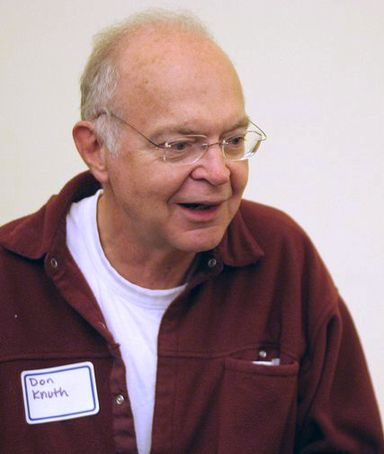
\includegraphics[scale=0.6]{images/Donald_Knuth.jpeg}
    \caption{克努斯博士,注:图片来源为克努斯博士的维基百科}
\end{figure}

由于克努斯博士此次在数学公式的排版上下足了功夫,就在他启动这项计划不久后,他收到了美国数
学协会 (American Mathematical Society, AMS) 的邀请,克努斯博士在此次邀请中汇报的内容
是“基于TeX排版,如何让计算机服务于数学”,这次汇报成功吸引了一大批数学家的目光。由于TeX
在数学公式排版方面的优秀表现,比如数学公式的自动间距调整,TeX后来摇身一变成为了书写数学
公式的“利器”。

为了提升TeX的开发质量,克努斯博士悬赏奖励任何能够在TeX中发现程序漏洞的人,也就是我们一般
认为的“找bug”。每一个bug的奖励金额从2.56美元(16进制的100美分)开始,以后每发现一个bug,
都会翻倍,直到327.68美元封顶。然而,克努斯博士从未因此而损失大笔金钱,因为TeX中的bug极
少,而真正发现bug的人在获得支票后往往因其纪念价值而不愿兑现。

随着时间的推移,TeX也派生出了很多优秀的软件,其中最著名的派生软件便是LaTeX。另外,美国
数学学会也发布了TeX版本的数学公式宏包,其中,以ams命名的宏包就有\emph{amsfonts}、
\emph{amsmath}、\emph{amssymb}等,这些宏包都可以在LaTeX上进行使用,在LaTeX上使用这
些宏包可以编辑出各种数学公式。

\begin{tcolorbox}[colback=red!5!white, colframe=red!50!black, title=参考资料]
    TeX的维基百科介绍: https://zh.wikipedia.org/wiki/TeX.
\end{tcolorbox}

\section{引领浪潮的\LaTeX }
\subsection{\LaTeX 的出现}
LaTeX是一款高质量的文档排版系统,LaTeX在读法上一般发作Lay-tek或者Lah-tek的音,而不
是大家普遍认为的Lay-teks。LaTeX的历史可以追溯到1984年,兰波特博士作为早期开发者在这一年
发布了LaTeX的最初版本。事实上,LaTeX完全是兰伯特博士的意外所得,他当年出于自己写书
的需要,在早先发布的文档排版系统TeX基础上新增了一些特定的宏包,为了便于自己日后可以重复
使用这些宏包,他将这些宏包进行规整,于是,便有了相应的标准宏包 (standard macro package)。
谁曾想,正是这些不经意间开发出来的宏包,在经过后续封装和发布使用手册之后,形成了LaTeX的
雏形。

\begin{figure}
    \centering
    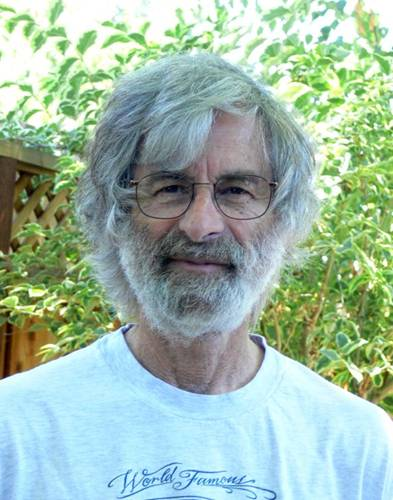
\includegraphics[scale=0.6]{images/Leslie_Lamport.jpeg}
    \caption{兰伯特博士,注:图片来源为兰伯特博士的维基百科}
\end{figure}

在很长一段时间里,LaTeX的版本其实没有多少大的更新,从技术层面来说,LaTeX实在没有什
么可供更新的地方了,它最初的面貌已趋近于完美且深入人心。LaTeX的最初版本是由兰伯特博士
于上世纪80年代初开发出来的,目前,广泛使用的版本LaTeX2e是在1994年发布的,发布后一直没有
大的更新,甚至发布后的首次更新出现在二十多年后的2020年。尽管LaTeX2e的后续版本更新工作早
在上世纪九十年代初就已经开展了,但时至今日,新版的LaTeX仍未进入人们的视野。从开发者兰伯
特博士的角度来看,开发LaTeX的目的是为了降低TeX的使用门槛、更容易地发挥TeX强大的排版功能,
提供一款高质量、解释性强的计算机程序语言,所以LaTeX最初的风格就是精简,这也是为什么LaTeX
在日后可供提升的地方不是很多的原因。

\subsection{\LaTeX 的特点}
由于种种原因,时至今日,TeX几乎淡出了人们的视线,不过我们现在依旧能看到:在使用LaTeX制作
文档时,通常需要创建一个以\emph{.tex}为拓展名的文件。对于很多人来说,日常制作各类文档的
首选可能是Word等软件,它简单好用、所写即所见,但当我们制作几十页甚至上百页的文档时,Word
的劣势就会展露无疑,因为我们需要投入大量的时间和精力来对文档内容进行排版。反观LaTeX,它
对文档的排版都是自动完成的,我们根本不需要像Word那样完全手动调整格式,另外,使用LaTeX插
入各种图形、表格、公式、文献时,相应的索引出错的可能性也非常小,这些优点都是Word所无法
比拟的。

在上个世纪80年代和90年代,LaTeX的用户群体非常庞大,然而,在世纪之交,随着微软推出的一系
列Windows操作系统快速发展,例如红极一时的XP系统,相应的办公软件Microsoft Office也以其
便捷性吸引了人们的视线,致使大量LaTeX用户转而使用Microsoft Office。即便如此,时至今日,
LaTeX的用户群体依旧十分庞大,这主要得益于LaTeX强大的文档排版能力,虽然LaTeX复杂的语法结
构、不容配置的编译环境让很多初学者望而却步,但LaTeX能让用户更专注于内容创作,而非锦上添
花的“排版”,这一显著特点契合了人们对质量和效率的追求,使得LaTeX在文档排版、论文撰写等方
面占有重要地位。在此基础上,具体来说,使得LaTeX历久弥新的关键可以归纳为以下五点:
\begin{enumerate}
    \item LaTeX是专门用于制作文档的计算机程序语言。在众多计算机程序语言中,LaTeX可以制
          作排版连贯性极好的专业文档。
    \item 独特的创作方式。尽管LaTeX沿用了TeX排版系统,但使用LaTeX制作文档时,内容创作
          和文档生成却是分开的,有需要的时候,我们可以预览创作的文档。因此,在创作的过程中,
          创作者不再像使用办公软件Word那样,既要关注创作内容,又要同步关注繁琐的排版和格式,
          使用LaTeX制作文档能在真正意义上让创作者专注于创作内容本身。更值得一提的是,当文档篇
          幅较大时,使用LaTeX无疑会让我们节省大量的时间和精力。
    \item 简单的逻辑结构。使用LaTeX制作文档时,创作者可以通过一些非常简单的逻辑结构进行
          创作,如chapter(章)、section(节)、table(表格)。因此,LaTeX的使用门槛并不像
          真正的程序语言那么高。很多人或许在使用LaTeX的过程中都不会用到for等基本的循环语句。
    \item 对数学公式以及特殊符号的支持程度。众所周知,LaTeX在开发之初,是作为数学和计算
          机相关研究人员的创作工具,这类群体喜欢使用LaTeX的原因无外乎是LaTeX可以通过一些简单
          的代码生成复杂的数学表达式和特殊符号。
    \item 编译以\emph{.tex}为拓展名的LaTeX文件后会得到一个PDF文档,PDF文档不存在跨
          平台、兼容性等问题,可以在各种操作系统上打开。
\end{enumerate}

当然,除了上述五点,实际上可能还有十分重要的一点,那就是LaTeX能够制作各类文档,从科技
论文、技术报告、著作、学位论文、幻灯片甚至到科技绘图一应俱全,当然它也支持嵌入图片、绘制
图形、设计表格、插入参考文献等。

从LaTeX的出现到当下,它已经形成了一套非常高效的文档制作环境:
\begin{itemize}
    \item 文档类型 (document class)。文档类型是文档排版样式的基调,这些类型包括
          文章 (article)、报告 (report)、幻灯片 (beamer)等,在.tex文件中申明文档类型后,
          我们就可以开始文档创作了。
    \item 宏包 (package)。它是LaTeX中的重要辅助工具,也可以把它理解为一般意义上的工具
          包。在使用时,调用宏包的基本命令为\emph{\textbackslash usepackage\{\}},举例来说,包含颜色命令的
          宏包为\emph{color},其调用语句为\emph{\textbackslash usepackage\{color\}}。随着LaTeX的发展,越来
          越多的宏包被开发出来,这些宏包能满足特定的需求(如制表、插图、绘图),同时也能让
          LaTeX代码变得更加简洁,我们只需要用简单的\emph{\textbackslash usepackage\{\}}命令就能调用
          所我们需要用到的宏包。
    \item 模板 (template)。LaTeX的发展催生了很多视觉和审美效果极好的模板,包括论文模板、
          幻灯片模板、报告模板甚至著作模板,这些模板在一定程度上能减少创作者在文档排版上的时间
          开销,也有很多学术刊物会给投稿作者提供相应的LaTeX模板。
\end{itemize}

通过对比LaTeX和Word,我们还会看到:
\begin{itemize}
    \item 第一,LaTeX的.tex源文件是无格式的,编译之后,根据特定的模板和指定的格式形成
          最终的PDF文档,因此,使用LaTeX制作各类文档能够很方便地切换模板和修改格式;
    \item 第二,LaTeX对公式、图表以及文献引用的支持是Word所无法比拟的,尤为特殊的是,
          当文献数量达到上百篇时,在Word中修改参考文献可能是“牵一发而动全身”,费时耗力,而
          LaTeX根据已经整理好的\emph{.bib}文件可自动完成文献引用和生成。
\end{itemize}

\subsection{\LaTeX 编辑器}
实际上,配置LaTeX环境包括两部分,即编译器和编辑器,对应的英文表达分别是editor和complier,
两者不是一回事。LaTeX编译器又称为LaTeX编译工具,可根据系统安装相应的编译工具:
\begin{itemize}
    \item Linux系统:可安装TeX Live,该编辑器拥有LaTeX编辑器;
    \item Mac OS系统:可安装Mac TeX,该编译器拥有完整的TeX/LaTeX环境和LaTeX编辑器;
    \item Windows系统:可安装MiKTeX或TeX Live,两者都拥有完整的TeX/LaTeX环境和LaTeX编辑器。
\end{itemize}

目前,我们可以接触到很多LaTeX编辑器,这些编辑器的界面大致有两部分组成,即LaTeX源码编译
区域和PDF文档预览区域。前面也提到了几款LaTeX编译器,但如果想要提高LaTeX的使用体验,以下
几款LaTeX编辑器比较受人推崇:
\begin{itemize}
    \item TeXworks:这是TeX Live自带的一款轻量级编辑器。
    \item TeXstudio:这款编辑器集代码编译与文档预览于一身。
    \item WinEdt:这是CTeX自带的一款编辑器。
    \item VS Code:这是微软推出的一款免费文本编辑器,功能包括文本编辑、日常开发等。
    \item Atom:这是一款开源的跨平台编辑器(GitHub网址为https://github.com/atom/atom),
          支持多种程序语言。
\end{itemize}

\section{应运而生的在线系统}
\subsection{\LaTeX 在线系统的出现}
上世纪80年代,LaTeX作为一件新生事物,在发布之初便引起了人们极大的兴趣,虽然在制作文档方
面拥有很多办公软件都无法比拟的强大优势,尤其在数学公式编写及高效排版上具有很大优势,但是
由于其较高的使用门槛(使用计算机程序语言进行编译)和安装成本(本地安装需要花费大量的时间
配置相应的环境),在很长一段时间里,LaTeX主要用户都是科研工作者。然而,LaTeX在线系统的
出现已实实在在地改变了这一尴尬局面。

随着信息技术快速发展、互联网深度普及,人们的工作生活方式也在发生着很大改变,很多过去安装
在本地的操作软件都被搬到了浏览器上,人们无须在个人计算机上安装各类办公软件就能进行办公,
这带来了极大的便利。不过这类在线系统也存在一些先决条件,例如,出于计算资源方面的考虑,通
常要求在线系统的类型不能是计算密集型,因为计算密集型的在线系统往往需要大量的计算资源作支
撑。反观LaTeX,尽管我们可以认为LaTeX是一种计算机程序语言,但实际上,其对计算资源的需求
并不是很大。

在过去,受网速限制,使用线上系统几乎是一件难以想象的事。然而,在线系统的兴起并非空穴来风,
一方面是目前的网速已经跟过去发生了质的变化,另一方面则是上网成本在急剧降低,互联网触手可
及,已经成为人们日常生活和工作中不可或缺的一部分。以前,我们可能已经习惯了在本地计算机上
安装和使用各类软件或者集成开发环境,不过以LaTeX为例,在本地计算机上安装的集成开发环境也
有很多缺陷:
\begin{itemize}
    \item 第一,我们需要为安装LaTeX编辑器腾出很大的存储空间;
    \item 第二,某些特定的宏包需要额外安装和配置,但安装过多宏包之后又会使LaTeX变得很臃肿,
          甚至是不友好;
    \item 第三,当我们在本地计算机使用LaTeX制作文档时,我们很难与合作者进行协同创作。
\end{itemize}

在这个背景下,一些成熟的LaTeX在线系统逐渐走进人们的视野,并受到很多用户的喜爱,其中,最
为著名的LaTeX在线系统便是\emph{overleaf.com}。这些LaTeX在线系统不仅支持各种语言、各种
拓展宏包等复杂的LaTeX环境,同时也支持实时编译和实时预览编译后的文档,就算是换一台电脑,
也丝毫不会影响创作过程,创作完成之后,可以选择下载压缩文件包(如.zip),也可以只导出PDF
文档,毫无疑问,这些人性化的设计都是为了让LaTeX更加便捷和高效。除此之外,现有的LaTeX在
线系统还提供大量的LaTeX模板库,科技论文、毕业设计、幻灯片、海报、简历等参考模板一应俱全,
就连LaTeX使用文档也数不胜数。

\begin{tcolorbox}[colback=red!5!white, colframe=red!50!black, title=在线系统 overleaf]
    Overleaf是一个初创的科技企业,它的主要业务是构建现代化协作创作工具,即LaTeX在线系统,
    旨在让科学研究变得更加便捷和高效。
    目前,Overleaf已合并另一款著名的LaTeX在线系统ShareLaTeX,在全球范围内拥有超过600万
    用户,这些用户大多是来自于高校和研究机构的研究人员、老师以及学生,只要打开网址overleaf.com,
    用户无需在本地计算机配置LaTeX环境就可以创建各种LaTeX项目。
    \tcblower
    关于Overleaf的介绍可参考https://www.overleaf.com/about。
\end{tcolorbox}

\begin{figure}
    \centering
    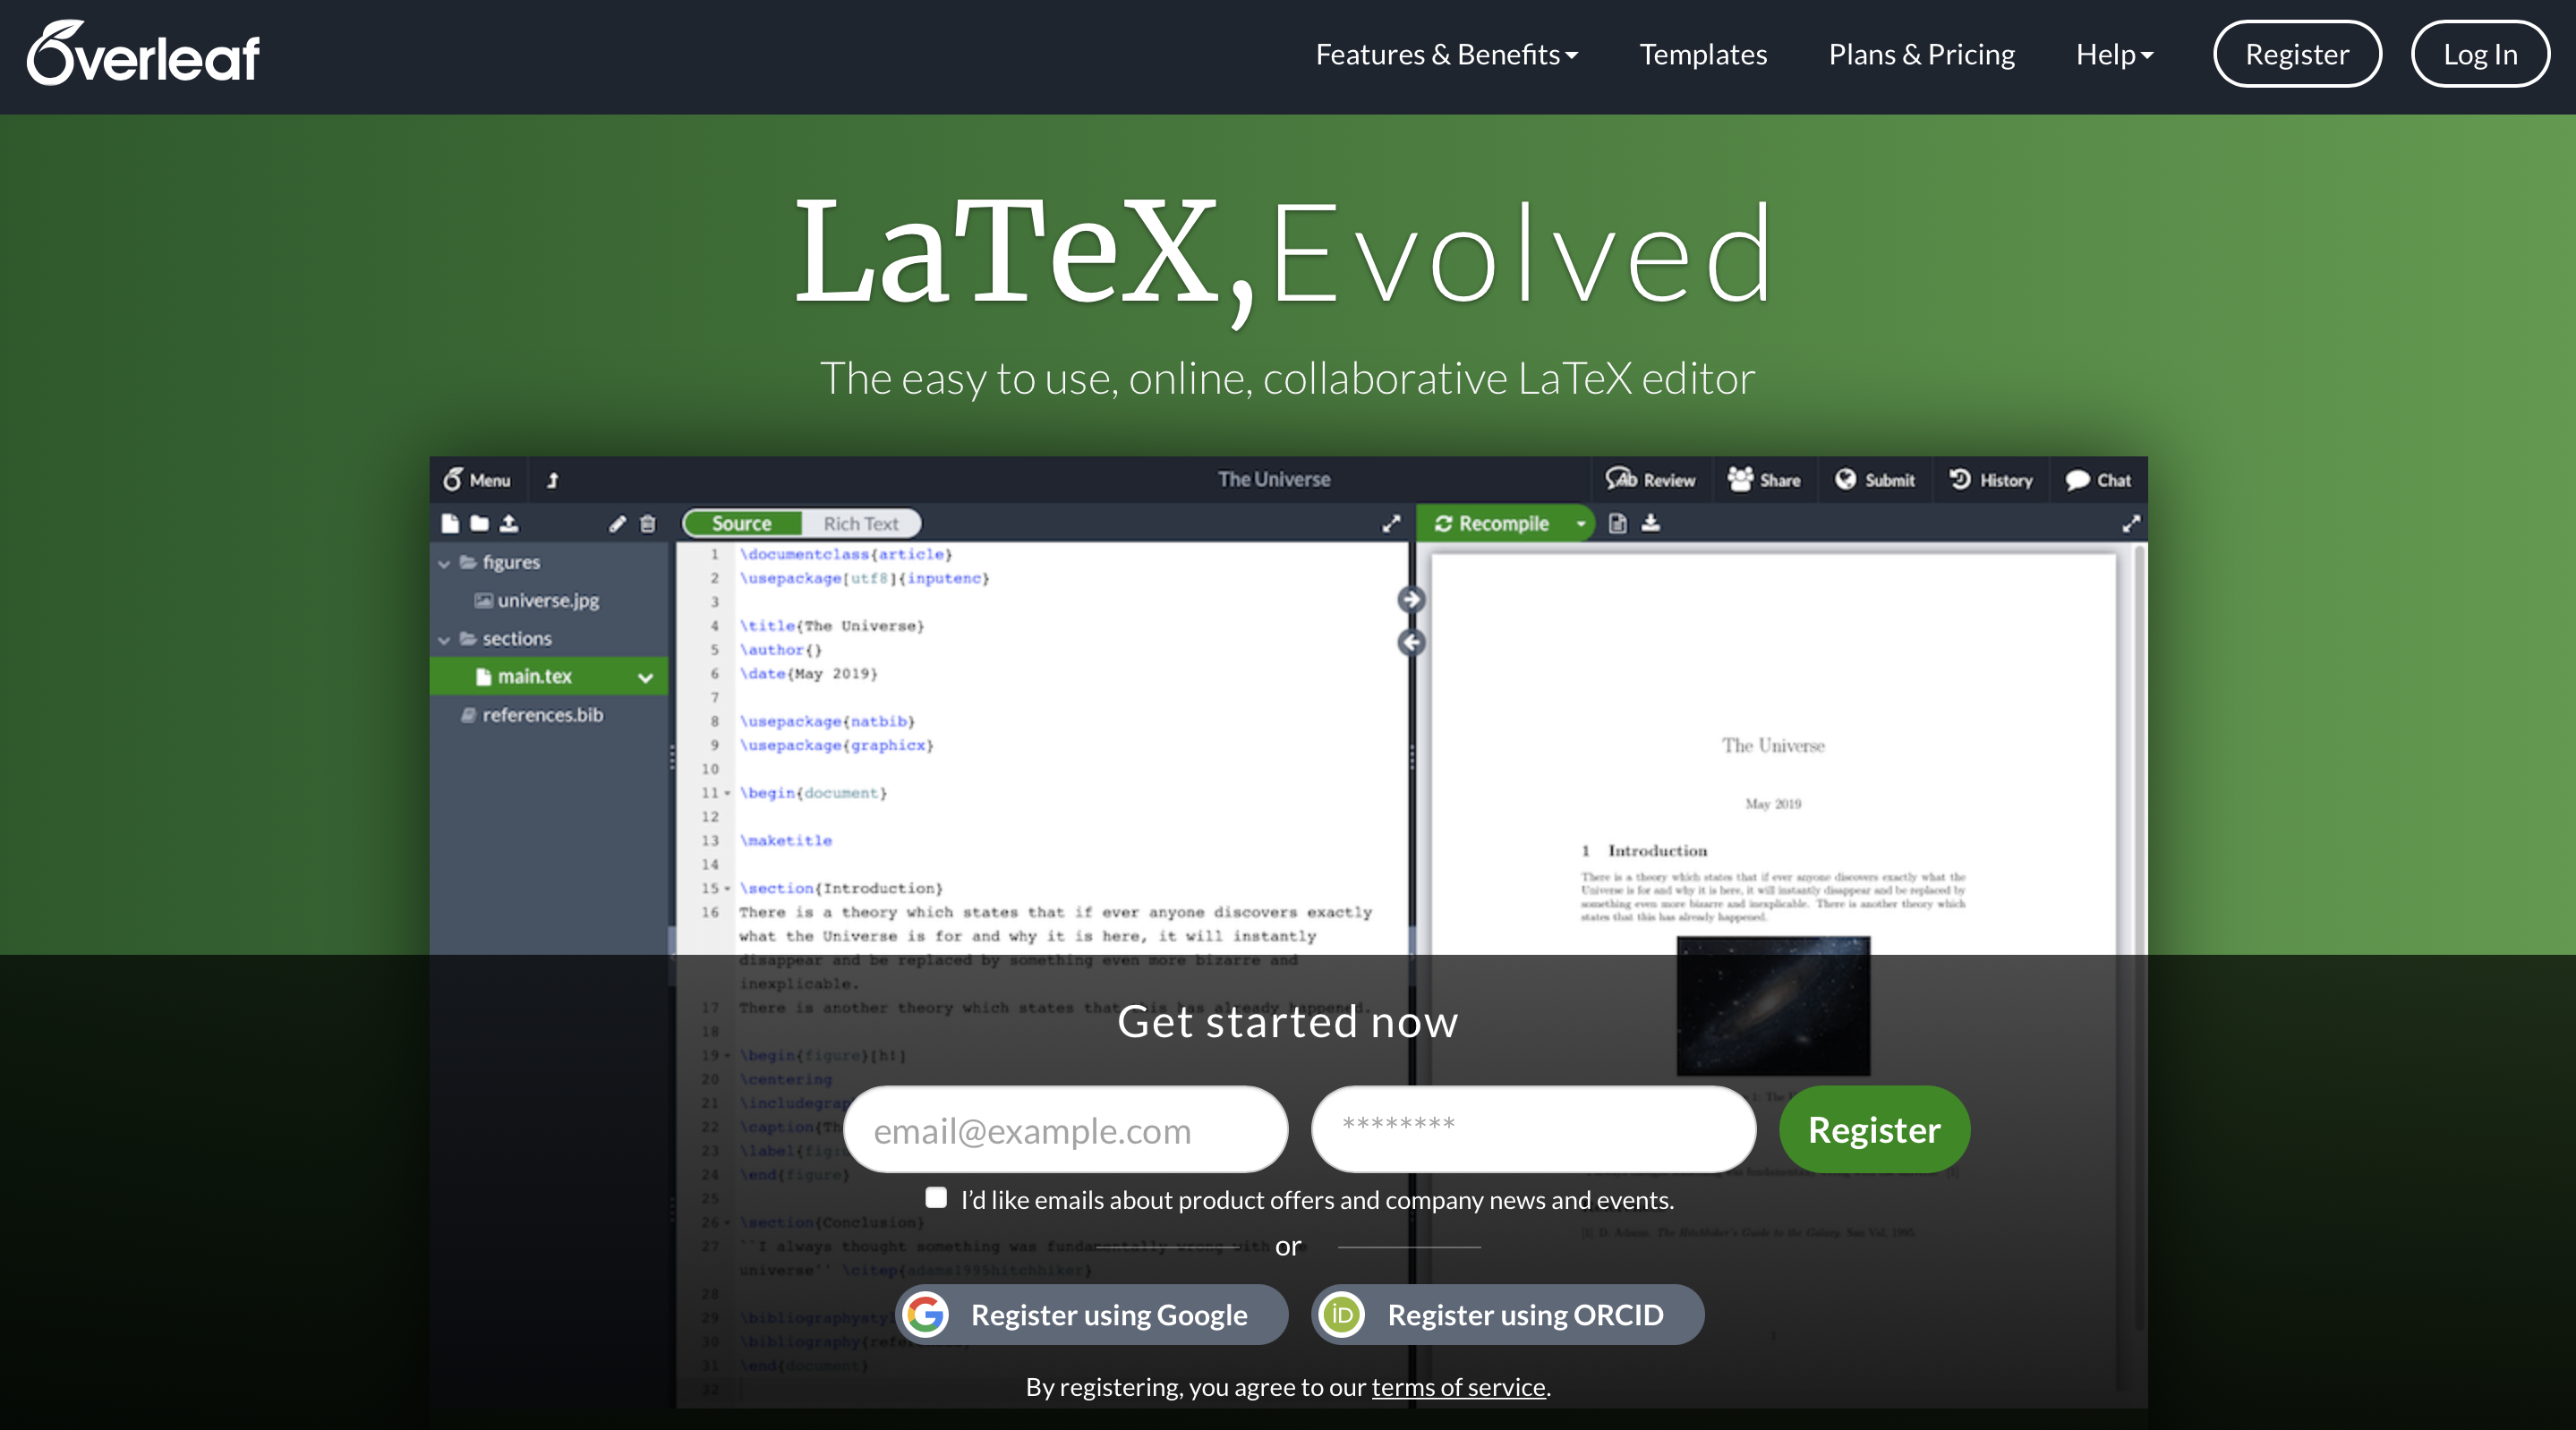
\includegraphics[width=\textwidth]{images/overleaf_webpage.png}
    \caption{Overleaf首页,图片来源于Overleaf官网}
\end{figure}

\subsection{\LaTeX 在线系统的特点}
以Overleaf为例,该LaTeX在线系统往往具备以下几点特征:
\begin{itemize}
    \item 免费和开源。可以免费注册和使用,不用下载和安装LaTeX编辑器,这一点对于初学者
          来说无疑是非常友好的;
    \item 使用简单。不管是在计算机、手机还是其他终端上,我们只需要使用浏览器打开overleaf.com
          就可以开始创作,另外,由于Overleaf界面非常简洁,所以用户使用起来也非常便利;
    \item 支持实时在线编辑。有各类LaTeX插件,编辑功能十分完善,且具有实时编译和预览功能;
    \item 支持在线协作。创作文档时,我们可以将文档项目分享给合作者进行协作,Overleaf支持实时编译,
          不会出现版本控制混乱等问题;
    \item 支持双向定位。可以在LaTeX代码与PDF文档内容之间进行双向定位;
    \item 提供丰富的模板库。Overleaf有着非常庞大的模板库,不仅有正式的学术论文、学位论文
          和书籍的参考模板,还有很多美观的报告、简历、幻灯片模板。就论文写作来说,用户可以在Overleaf
          官网找到众多期刊的LaTeX模板,根据使用说明,用户很容易就能用于撰写自己的论文;
    \item 提供大量的帮助文档。LaTeX提供了齐全的帮助文档,从LaTeX快速入门、基础操作到编译
          数学公式,应有尽有、一应俱全,且这些文档内容具有很强的实操性。
\end{itemize}

\begin{figure}
    \centering
    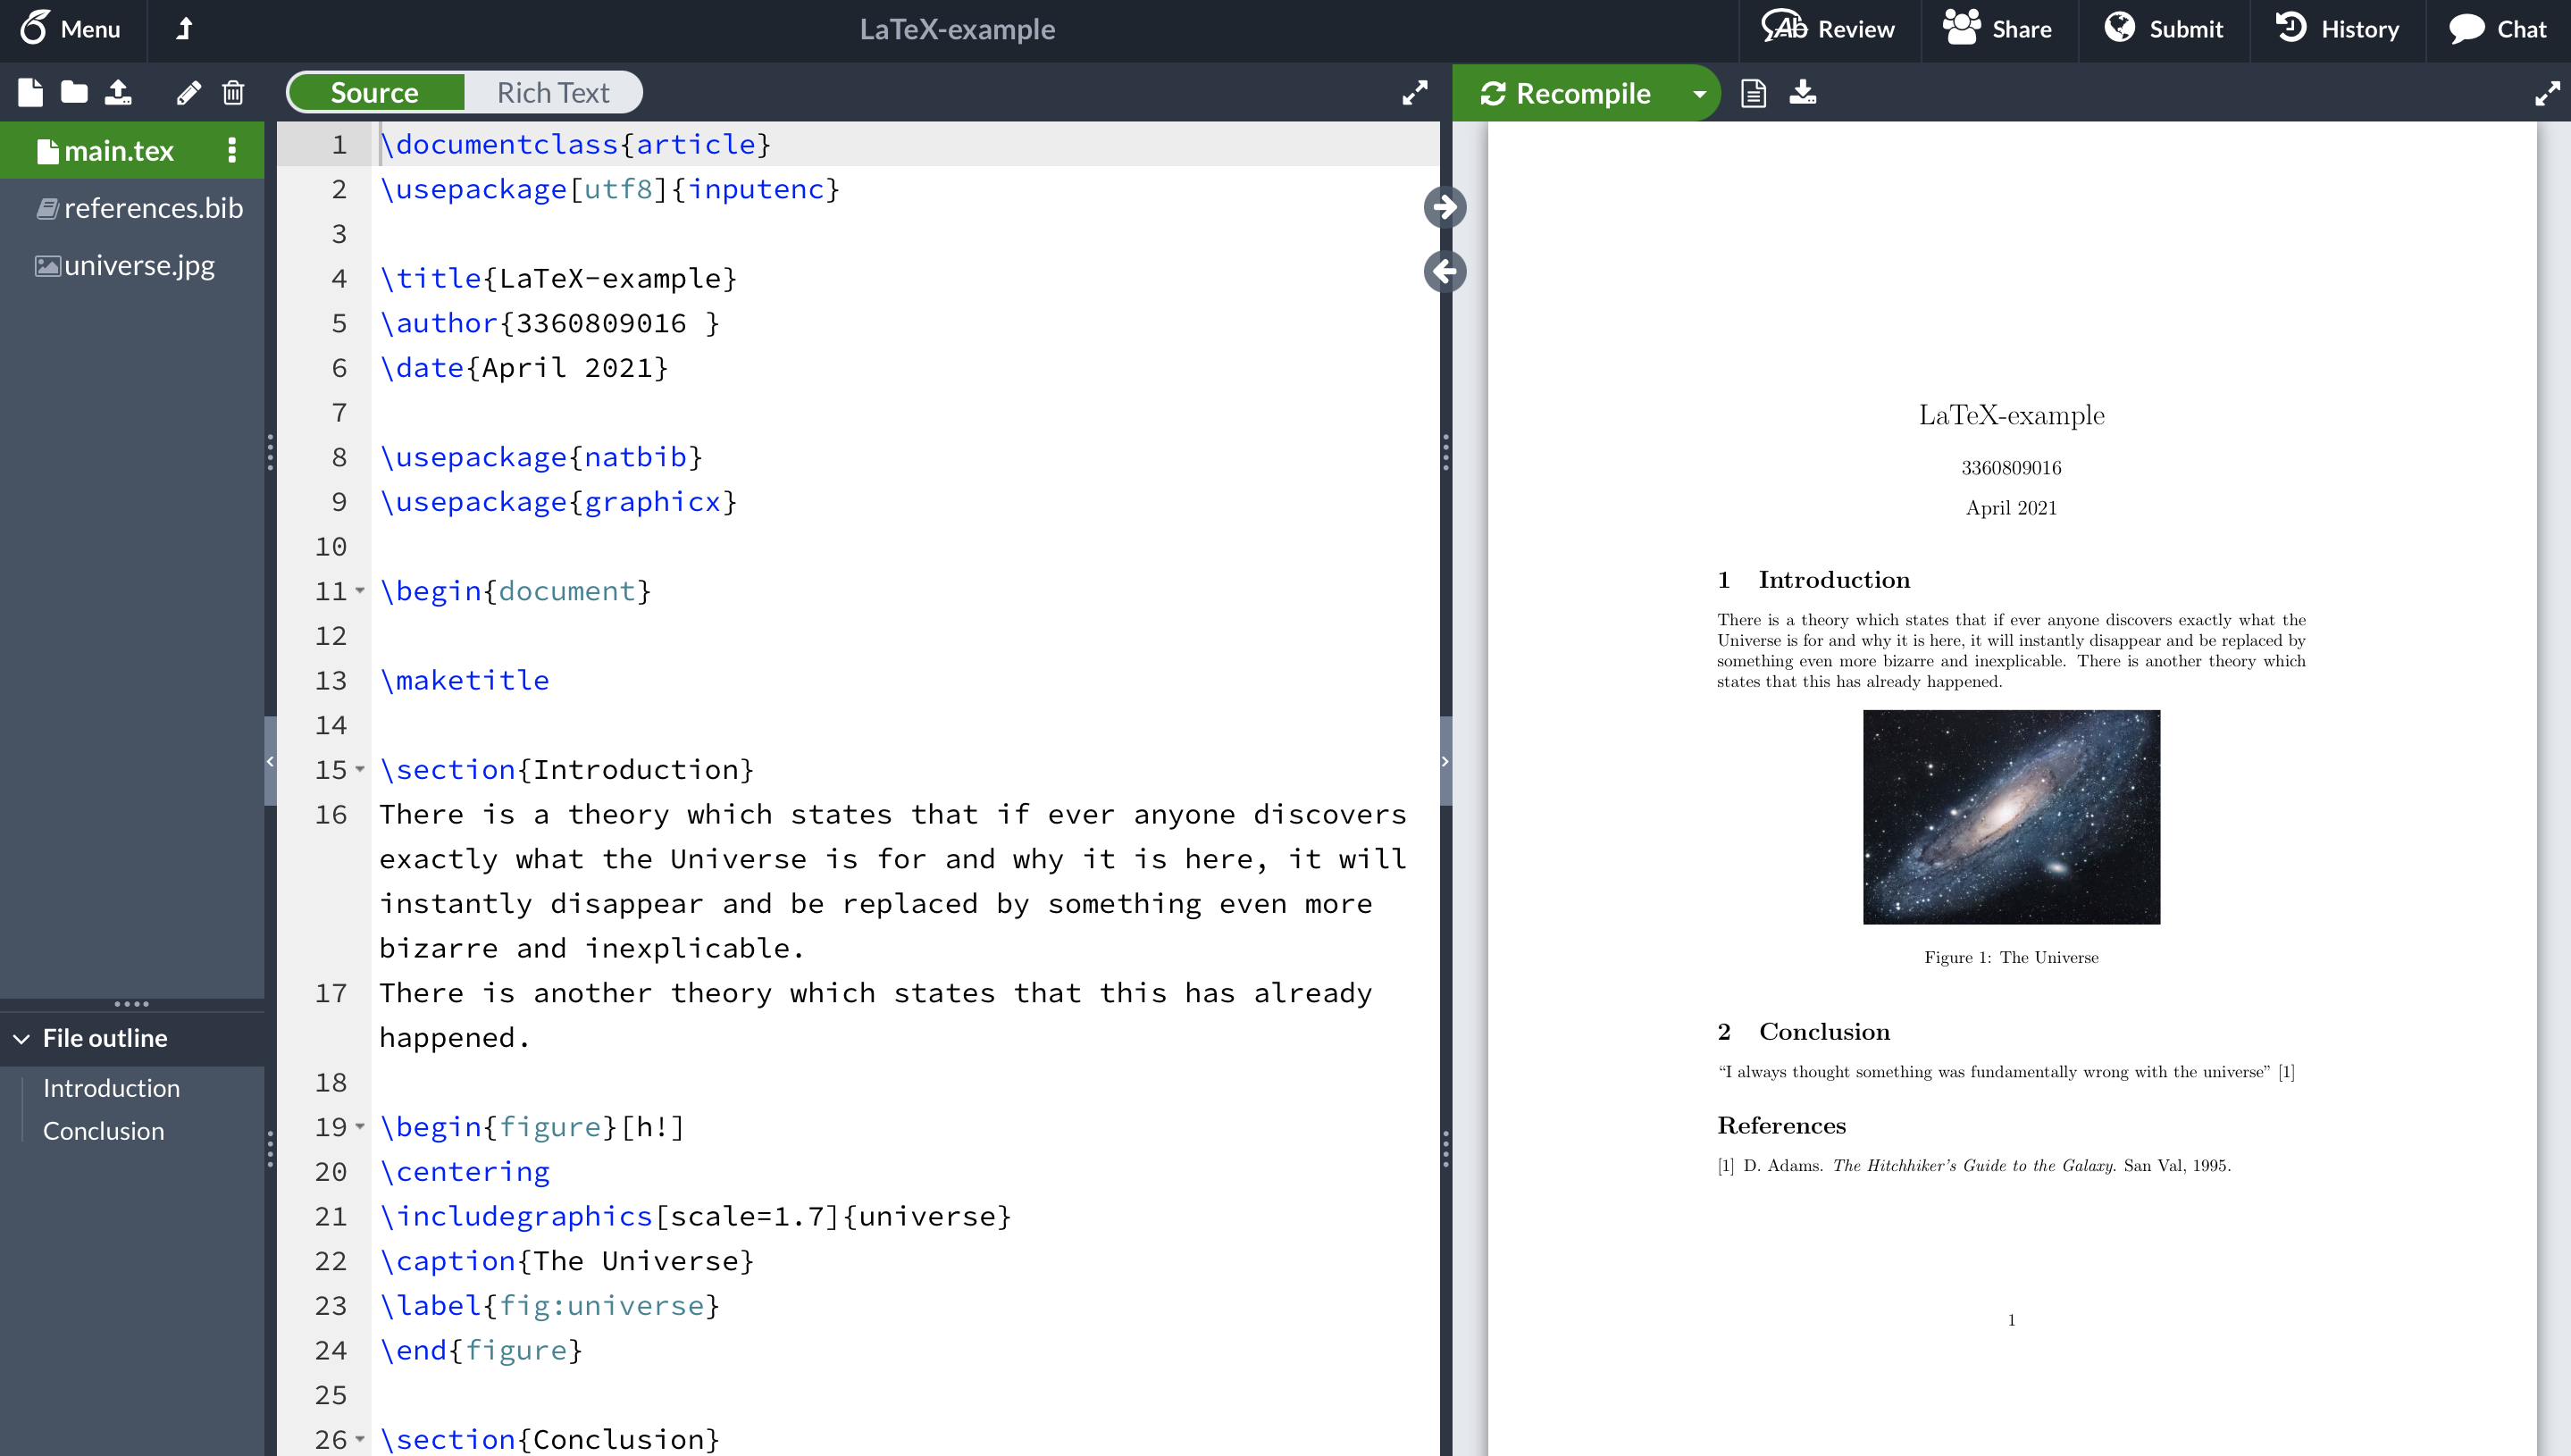
\includegraphics[width=\textwidth]{images/overleaf_example.png}
    \caption{Overleaf编辑器界面,主要由代码区域和文档预览区域组成}
\end{figure}

LaTeX在线系统的出现大大降低了LaTeX的使用门槛,也为用户省去了繁琐的安装和配置过程。其实,
LaTeX在线系统的出现并非个例,很多办公软件为迎合用户需求和时代发展趋势,陆续转变了产品研
发思路,包括微软在线Office系统、腾讯在线文档等在内的很多在线系统都走进了人们的视野,这些
在线系统能够在线备份、满足人们对随时随地办公的需求,在确保便捷和高效的同时,在线和共享的
理念正在潜移默化地影响着人们的办公模式。

\section{\LaTeX 问答社区}
在LaTeX刚被发布和推出的那个年代,相关资源如使用手册、教程等远没有今天这么丰富,同时,获
取渠道也没有今天这么便捷。在互联网触手可及的今天,我们能通过一个浏览器访问到各种相关学习
素材,遇到代码bug,也能在一些专业的问答社区找到最佳的解决方案。毫无疑问,对于今天的我们
来说,如何利用好互联网资源至关重要。

\subsection{问答社区的介绍}
对于从事计算机相关的技术人员来说,专业的技术问答社区往往是不可多得的资源,它能帮助很多技
术人员提升个人编程能力、学习新技术,同时解决一些技术困扰,例如解决编程时遇到的bug。对于
各类计算机程序语言而言,\emph{Stack Exchange}作为一个著名的技术问答社区,覆盖了大量编
程相关的技术问题和优质回答,就算是一些较为细致的问题,我们往往都能找到想要的答案。
Stack Exchange问答社区按计算机程序语言类型进行划分,我们所关心的LaTeX问答通常被分配在
TeX Stack Exchange社区(网址为https://tex.stackexchange.com/)。截至目前,
TeX Stack Exchange已经覆盖了关于TeX、LaTeX以及其他排版系统的用户在使用中遇到的诸多问题,
并且这些问题多与LaTeX相关。

\begin{tcolorbox}[colback=red!5!white, colframe=red!50!black, title=Stack Exchange]
    网址为https://stackexchange.com/,它与Stack Overflow问答社区在全球范围内拥有广泛的用户群体
\end{tcolorbox}

除了Stack Exchange这种涵盖了多种计算机程序语言的技术问答社区,LaTeX forum社
区(https://latex.org/forum/)是一个专门面向LaTeX的技术交流平台,它拥有非常活跃的用户
群体和丰富的问答资源,并拥有超过10万篇分门别类的技术帖子,我们可以根据浏览量从该平台一
览高频访问问题。

实际上,不管是LaTeX初学者还是高级用户,在遇到LaTeX使用问题时,去问答社区寻找解决方案都
是一种非常有效的方式。TeX Stack Exchange社区非常活跃,每天都会有大量关于LaTeX的问题和
回答,且每个问题下面的回答都会根据用户的认可度进行排序,回答一般比较细致。

\subsection{高频访问问题}
顾名思义,高频访问问题是指访问量较高的问题。LaTeX forum社区已经将众多问答帖子进行了分门
别类整理,针对某一特定话题,展开内容即可看到各类问题的访问情况。

\section{关于\LaTeX 的开源项目}
实际上,不管是TeX还是LaTeX,它们作为计算机程序语言是完全开源的,我们可以轻松获取到TeX
和LaTeX的源代码。近些年来,互联网催生了一些用户体验以及评价很好的开源社区,比如当下非常
受欢迎的开源平台GitHub,它们都在实实在在地影响着我们对于计算机技术开放的态度。开源社区
有很多优质的“仓库” (repository),这些仓库会提供诸如源代码、工具、案例甚至使用文档。与
LaTeX在线系统相似的是,这些开源社区非常支持协作功能,在有一些优质的仓库中,我们或许能看
到几十甚至上百个贡献者,“汇聚集体智慧”也是这些开源社区广受开发者青睐的一个重要原因。

\subsection{开源社区GitHub}
GitHub是一个面向开源项目及私有项目的云端托管平台,官方网址为http://github.com/,旨在为
开发者储存、管理代码以及控制代码的更新,只支持Git作为唯一的版本库格式进行托管。GitHub已
经走进人们的视野已经有十几年了,它于2008年4月10日正式上线,除了Git代码仓库托管和基本的
网页管理界面以外,还提供了在线文件编辑器、版本控制、协作报表等功能。截至2021年初,GitHub
在全球范围内拥有的注册用户已经超过5000万,托管项目的总量更是超过1亿,是很多开发者远程协作
的重要工具。2018年6月,GitHub被微软以75亿美元的价格收购。

GitHub本着开源、共享、协作的理念正影响着开发社区生态,吸引了包括微软和谷歌等国外技术巨头
在这里进行开源,另外,我们也能在GitHub上看到一些国内互联网企业的身影。实际上,GitHub开源
社区的项目类型及展现形式也异常丰富,既有大量的应用型项目,也有很多研究探索型项目。

为了方便开发者追踪整个开源社区的开发动态,GitHub根据计算机程序语言类型提供了趋势分析,这
个功能称为GitHub trending,它会定期更新趋势榜、帮助开发者追踪当下较为流行的GitHub仓库。

GitHub开源社区提供了很多关于LaTeX的优质开源项目,这些项目使得LaTeX的用户群体越来越广泛。
实际上, LaTeX在线系统Overleaf也是开源的,它托管在GitHub上,
网址为https://github.com/overleaf/overleaf。

为便于读者认识和掌握LaTeX,以下简单归纳一下关于LaTeX的各类开源项目。需要注意的是,优质的
开源项目是非常多的,限于篇幅,这里只列举一部分,感兴趣的读者不妨在GitHub平台上探寻更多
优质项目。

\subsection{学位论文\LaTeX 模板}
在GitHub开源社区中,我们可以找到很多国内外高校官方和非官方的学位论文LaTeX模板,学位论文
类型包括本科毕业设计、硕士学位论文和博士学位论文等。以下将列举一部分国内高校的学位论文
LaTeX模板开源项目:
\begin{itemize}
    \item 开源项目https://github.com/tuna/thuthesis提供了清华大学学位论文LaTeX模板,
          模板库涵盖本科综合论文训练、硕士论文、博士论文以及博士后出站报告,截至目前,已在
          GitHub上获得超过3000次标星。
    \item 开源项目https://github.com/mohuangrui/ucasthesis提供了中国科学院大学学
          位论文LaTeX模板,包括本科、硕士和博士学位论文模板,截至目前,已在GitHub上获得超
          过2000次标星。
    \item 开源项目https://github.com/mohuangrui/ucasthesis提供了中国科学院大学学
          位论文LaTeX模板,包括本科、硕士和博士学位论文模板,截至目前,已在GitHub上获得超
          过2000次标星。
    \item 开源项目https://github.com/ustctug/ustcthesis提供了中国科学技术大学学位
          论文LaTeX模板,包括本科毕业论文(设计)和研究生学位论文,截至目前,已在GitHub上
          获得近1000次标星。
    \item 开源项目https://github.com/TheNetAdmin/zjuthesis提供了浙江大学学位论文
          LaTeX模板,包含本科、硕士和博士学位论文模板,也提供了英文版的硕博士学位论文模板,
          截至目前,已在GitHub上获得近1000次标星。
    \item 开源项目https://github.com/dustincys/hithesis提供了哈尔滨工业大学学位论
          文LaTeX模板,包括本科、硕士、博士开题、中期和毕业论文,也提供了博后出站报告和英文
          毕业论文格式,截至目前,已在GitHub上获得近1000次标星。
    \item 开源项目https://github.com/x-magus/ThesisUESTC提供了电子科技大学毕业论
          文LaTeX模板,截至目前,已在GitHub上获得超过500次标星。
\end{itemize}

上述开源项目提供的学位论文模板绝大多数支持在LaTeX在线系统overleaf.com上直接进行编辑和使用。

\subsection{\LaTeX 绘制图形}
目前,LaTeX有很多关于绘制图形方面的宏包,这些宏包会提供图形的基本元素、颜色等。由于LaTeX
绘制出来的图形可以以PDF文档保存,所以一般不会出现分辨率不足等问题。这里对LaTeX绘制图形
相关的一些开源项目稍作整理:

\begin{itemize}
    \item 工具类:
          \begin{itemize}
              \item \emph{BayesNet}:用于绘制贝叶斯网络、图模型和因素图形的TikZ库。开源网址
                    为https://github.com/jluttine/tikz-bayesnet。一般而言,使用BayesNet绘制特定图
                    形时,需要使用以下两行命令调用该库:\emph{\textbackslash usepackage\{tikz\}}和
                    \emph{\textbackslash usetikzlibrary\{bayesnet\}}
              \item \emph{matlab2tikz}:将由Matlab代码绘制的图形转换成PGFPlots图形。开源网
                    址为https://github.com/matlab2tikz/matlab2tikz。
              \item \emph{tikzplotlib}:将由Python绘图工具matplotlib绘制的图形转换成PGFPlots
                    图形。开源网址为https://github.com/nschloe/tikzplotlib。
              \item \emph{svg2tikz}:将SVG图形转换成TikZ代码。开源网址为https://github.com/xyz2tex/svg2tikz。
          \end{itemize}
    \item 实例类:
          \begin{itemize}
              \item \emph{TeXample}:该项目提供了大量的TikZ绘图实例,开源网址为https://texample.net/tikz/。
              \item 开源项目https://github.com/walmes/Tikz提供了大约200个关于统计学的TikZ绘图实例。
              \item 开源项目https://github.com/MartinThoma/LaTeX-examples/tree/master/tikz提供了大约350个TikZ绘图实例。
              \item 开源项目https://github.com/PetarV-/TikZ提供了大量的Tikz绘图实例,囊括了各类神经网络模型的图形。
              \item TeX Stack Exchange社区中提供的可视化效果很好的TikZ科技绘图实例,网址
                    为https://tex.stackexchange.com/questions/158668/nice-scientific-pictures-show-off。
              \item 开源项目https://github.com/FriendlyUser/LatexDiagrams提供了大量的TikZ绘图实例,包括
                    流程图、图模型。
              \item 开源项目https://github.com/alemelis/tikz\_drawings提供了一些TikZ绘图实例。
          \end{itemize}
\end{itemize}

\subsection{\LaTeX 制作简历}
LaTeX可用于制作各类文档,这也包括简历。

\begin{itemize}
    \item 开源项目https://github.com/sb2nov/resume提供了简历模板。
    \item 开源项目https://github.com/xdanaux/moderncv提供了moderncv简历样式。
    \item 开源项目https://github.com/jankapunkt/latexcv提供了一些美观大方且容易使用的简历模板,支持包括中文在内的多种语言编译。
    \item 开源项目https://github.com/hijiangtao/resume提供了中文简历的模板。
\end{itemize}

\subsection{\LaTeX 制作幻灯片}
\begin{itemize}
    \item 开源项目https://github.com/matze/mtheme提供了现代风格主题的幻灯片模板。
    \item 开源项目https://github.com/wzpan/BeamerStyleSlides提供了很丰富的模板,包含了PowerPoint和Keynote两套格式。
    \item 开源项目https://github.com/XiangyunHuang/awesome-beamers提供了多种制作幻灯片的模版,同时也支持中文制作。
    \item 开源项目https://github.com/josephwright/beamer提供了多种风格的幻灯片模版。
\end{itemize}

\subsection{\LaTeX 制作海报}
\begin{itemize}
    \item 开源项目https://github.com/jkjaer/aauLatexTemplates提供了beamer海报模板。
    \item 开源项目https://github.com/mloesch/baposter提供了简洁的海报模版。
    \item 开源项目https://github.com/HolgerGerhardt/TeXTemplates提供了适合做学术报告的海报模版,同时也包含幻灯片模版。
\end{itemize}

\subsection{推荐指导本书的开源项目}
开源网址为https://github.com/xinychen/latex-cookbook。同时该作者还有图形绘制和幻灯片
制作的开源项目:
\begin{itemize}
    \item LaTeX图形绘制:https://github.com/xinychen/awesome-latex-drawing提供大
          量绘图实例,实例包括贝叶斯网络、框架图、流程图、机器学习模型示意图。
    \item LaTeX幻灯片制作:https://github.com/xinychen/awesome-beamer提供大量使用
          Beamer制作幻灯片的实例。
\end{itemize}

\begin{tcolorbox}[colback=red!5!white, colframe=red!50!black, title=参考资料]
    开源项目https://github.com/xiaohanyu/awesome-tikz。
\end{tcolorbox}

\section{\LaTeX 制作中文文档}
LaTeX最初只提供英文的编译环境,随着其在文档编辑领域的优势越来越深入人心,更多国家的学者
希望用到这一工具,因此出现了许多支持各国语言的工具包或编写环境,作为全世界使用人数最多的
语言,LaTeX有\emph{CJKutf8}宏包、\emph{CTEX}宏包等多种方式可以实现中文文档编辑,均能
在开源网站Overleaf中调用并实现中文文档制作。

\subsection{使用CJKutf8宏包}
\emph{CJKutf8}宏包提供了两种中文简体字体制作中文文档:使用\emph{\textbackslash begin\{CJK\}\{UTF8\}\{gbsn\}}
和\emph{\textbackslash end\{CJK\}}环境将以宋体(gbsn)制作文档,而使用\emph{\textbackslash begin\{CJK\}\{UTF8\}\{gkai\}}
和\emph{\textbackslash end\{CJK\}}环境则以楷体(gkai)制作文档内容。在默认的pdfLaTeX
编译环境中即可得到文档编译结果。

\emph{【例】}使用\emph{CJKutf8}红包制作中文文档:
\begin{lstlisting}[language=TeX, caption={CJKutf8示例}]
\documentclass{article}
\usepackage{CJKutf8}

\begin{document}

\begin{CJK}{UTF8}{gbsn} %字体是gbsn
你好,LaTeX!。
\end{CJK}

\end{document}
\end{lstlisting}

\subsection{使用CTEX宏包}
CJKutf8宏包只提供了两种字体,可选择的余地太小。如果想要使用更丰富的字体编辑 Latex 中文
文档,可以调用\emph{CTEX}宏包、并设置UTF8选项使其支持utf-8编码。在Overleaf中使用CTEX
宏包时,需要先将编译环境从\emph{pdfLaTeX}调整为\emph{XeLaTeX}。
\emph{【例】}使用\emph{CTEX}宏包制作中文文档:
\begin{lstlisting}[language=TeX, caption={CTEX示例}]
\documentclass[UTF8]{ctexart}

\begin{document}

{\kaishu 你好,LaTeX!(楷体)}

{\songti 你好,LaTeX!(宋体)}

{\heiti 你好,LaTeX!(黑体)}

{\fangsong 你好,LaTeX!(仿宋)}。

\end{document}
\end{lstlisting}

目前在Overleaf上已经出现了许多中文文档LaTeX模板,除了一些学位论文模板,一些中文学术期刊
如《计算机学报》也提供了科技论文的LaTeX模板。

\textbf{期刊模板:}
\begin{itemize}
    \item 《中国科学:信息科学》https://www.overleaf.com/project/5e99712a0916c900018d11af
    \item 《中国科学:信息科学》https://www.overleaf.com/project/5e99712a0916c900018d11af
\end{itemize}

\textbf{中文学位论文模板:}
\begin{itemize}
    \item 《浙江大学学位论文模板》https://www.overleaf.com/project/610fa05007d0073d5405a04f
    \item 《武汉大学博士学位论文模板》https://www.overleaf.com/project/610fa09e07d007fa5605a1e9
    \item 《武汉大学博士学位论文模板》https://www.overleaf.com/project/610fa09e07d007fa5605a1e9
    \item 《南京大学研究生毕业论文模板》https://www.overleaf.com/project/610fa1d007d00704c305a3eb
\end{itemize}

另外,开源项目https://github.com/MCG-NKU/NSFC-LaTex提供了国家自然科学基金申报书的LaTeX模板。

% \chapter{\LaTeX 基础介绍}
\section{导言}
LaTeX作为专门用于制作文档的计算机程序语言,其语法规则是由命令 (command) 和环
境 (environment) 构成,基于一些基本命令,如\textbackslash usepackage\{\},我们能调用制
作文档所需的宏包。一般而言,在制作文档时,LaTeX的代码结构分为前导 (preamble) 和主
体 (body) 两部分,前导部分的代码主要用于申明文档类型、排版样式、所使用的宏包等;主体部
分主要用于确定标题、章节、目录等文章结构及创作文档内容。

掌握一些常用命令之后,我们便可上手编辑简单的文档。从功能上来说,LaTeX能满足人们对文档制
作多样性的要求。我们可以用LaTeX制作各类文档,包括科技文档、技术报告、学位论文、书籍著
作、幻灯片、个人简历、信件以及海报。不同的文档类型在文档大小、排版、章节样式方面略有不
同,所以在使用LaTeX制作文档时,我们首先需要对文档类型进行申明,然后再进行文档内容的创作。

本章节要介绍的内容主要包括:Latex语法规则、Latex代码结构、文档类型的介绍、简单文档的制
作以及全局格式的设置。

\section{\LaTeX 语法规则}
对于任何一种计算机程序语言,严格的语法规则都是让程序语言实现功能的保障。不同于一般性的计
算机程序语言,LaTeX的语法规则非常简单,是由命令和环境构成。在LaTeX中,不管是命令还是环
境,都离不开计算机符号反斜线\textbackslash,例如调用宏包会用到
\textbackslash usepackage\{宏包名称\},这里的花括号\{\}也是非常常用的一个符号。在调用宏包
后,命令的用法都是由宏包约定的。

\subsection{命令}
LaTeX中有很多命令,它们用法大同小异,功能却千差万别。既有申明文档类型的命令,如\textbackslash documentclass\{article\},
也有输入特殊符号的命令,例如\textbackslash copyright。一般而言,LaTeX中的命令通常由三
部分组成\textbackslash 命令名[可省略参数]\{不可省略参数\},具有以下特点:
\begin{itemize}
    \item 通常都是以反斜线作为开始,通过紧跟的既定字符(命令名)实现相应的功能,例
          如\textbackslash LaTeX和\textbackslash copyright可生成特殊字符。
    \item 一些命令需要申明一些参数,通过大括号中的不可省略参数进行申明,例如\textbackslash color\{blue\}
          命令中需要申明具体的颜色名称。
    \item 一些命令包括一些选项和一些参数一般情况下是默认的,有需要时可以通过中括号中的
          可省略参数进行调整,例如在\textbackslash documentclass[a4paper]\{article\}中,中
          括号[]作为额外的选项,既可以自行设置,也可以选择默认设置。
    \item 有些命令可以用反斜线作为终止,例如\textbackslash copyright。
\end{itemize}

\subsection{环境}
这里所说的“环境”是指编译环境,使用LaTeX时,当我们想要编译出期望的效果,例如列表、插入图
形、制作表格,我们就需要用到一些环境。举例来说,我们可以通过
\begin{lstlisting}[language=TeX]
    \begin{itemize}
        \item item 1 % 条目1
        \item item 2 % 条目2
    \end{itemize}
\end{lstlisting}

制作一个简单的无序列表,这里的\emph{itemize}表示无序列表环境,\emph{\textbackslash begin\{\}}
和\emph{\textbackslash end\{\}}表示环境的初始化和结束。当然,这些环境并非“一成不变”,我
们也可以设置一些参数,从而改变编译之后的文档效果,例如,可以通过
\begin{lstlisting}[language=TeX]
    \begin{spacing}{1.3}
        paragraph 1 % 第1段

        paragraph 2 % 第2段
    \end{spacing}
\end{lstlisting}
将两段话之间的行间距设置为1.3倍。

\emph{【例】}使用基本命令\textbackslash documentclass{article}和文档环境\textbackslash begin\{document\}
和\textbackslash end\{document\}创建一个简单文档。
\begin{lstlisting}[language=TeX]
    \documentclass{article}

    \begin{document}

    Hello, LaTeXers! This is our first LaTeX document.

    \end{document}
\end{lstlisting}

\subsection{宏包}
宏包是LaTeX的重要组成部分,用来扩展和增强LaTeX的功能,是支撑LaTeX实现一系列复杂文档编辑
和排版的关键所在。宏包与LaTeX的关系和浏览器插件与浏览器的关系类似,通过调用不同的宏包可
以实现一些复杂排版功能,例如插入表格、插入公式和特殊符号、插入程序源代码、设置文档样式等。
一个宏包通常会提供一组LaTeX命令,有些特殊命令只能在调用宏包后使用。在LaTeX中,调用宏包的
形式大同小异,如果想要使用某一特定宏包,最简单的办法就是用\textbackslash usepackage\{宏包名\}
命令对相应宏包进行调用。

\emph{【例】}使用\textbackslash usepackage\{color\}命令调用颜色宏包调整文本字体颜色。
\begin{lstlisting}[language=TeX]
    \documentclass{article}
    \usepackage{color} % 调用颜色宏包
    \begin{document}
    \textcolor[rgb]{1,0,0}{Hello, LaTeXers! This is our first LaTeX document.}
    \end{document}
\end{lstlisting}

\section{\LaTeX 代码结构}
在使用LaTeX进行文档编辑时,我们通常在拓展名为\emph{.tex}的源文件中书写代码,然后通过编译,生成
一个PDF格式的文档。LaTeX源文件的代码结构主要包含两个部分,即前导代码(preamble)和主体
代码(body),其结构示例如下:
\begin{lstlisting}[language=TeX]
    \documentclass[]{}

    ...... % 前导代码(preamble)

    \begin{document}

    ...... % 主体代码(body)

    \end{document}
\end{lstlisting}

\subsection{前导代码}
前导代码是指从源文件第一行代码到\textbackslash begin\{document\}之间的所有命令语句,
一般为LaTeX代码的第一部分。在前导代码部分,既可设置文档类型全局参数,包括字体大小、纸张
大小、文字分栏、单双面打印设置等,也可声明主体代码中需要用到的宏包,如插入图形、新增表格
所要用到的宏包。当全局格式没有特殊申明时,前导代码中的文档类型申明语句可以简写成\textbackslash documentclass\{B\},
其中,位置B的作用在于申明文档类型,如article(常规文档)、book(书籍)、report(报告)、
beamer(幻灯片)等。

下面以常规文档(article)为例,简要介绍各常用全局参数的设置方式。

\subsubsection{字体大小}
article类型文档字体大小默认为\emph{10pt},可在\textbackslash documentclass[可省参数]\{article\}
的中括号中根据需要设置成11pt和12pt。

通常,我们按照\textbackslash documentclass[fontsize = 12pt]\{article\}这样的形式设
置文档参数,有时候,为了方便起见,可以把文档类型申明做一定的简写,如\textbackslash documentclass[12pt]\{article\}。
需要注意的是,字体大小设置中的基本单位pt是英文单词point的缩写,是一个物理长度单位,
\textbf{指的是72分之一英寸,即1pt等于1/72英寸}。

\subsubsection{纸张大小}
article类型文档纸张大小默认为\emph{letterpaper},同样可在\textbackslash documentclass
    [可省参数]\{article\}的中括号中根据需要设置成\emph{a4paper}、\emph{a5paper}、\emph{b5paper}、
\emph{legalpaper}和\emph{executivepaper}。

\subsubsection{文字分栏}
article类型文档的文字分栏默认为\emph{onecolumn}(不分栏),也可以使用\emph{twocolumn}
参数设置为twocolumn(两栏)。

\subsubsection{单双面打印设置}
article类型文档打印时默认单面打印,同样可以使用\textbackslash documentclass[可省参数]
\{article\}中括号中的可选参数,通过添加\emph{twoside}参数进行双面打印的设置。

\begin{tcolorbox}[colback=red!5!white, colframe=red!50!black, title=文档属性设置小结]
    基于上面介绍可供调整的参数,我们可以进行任意无序组合,例如\textbackslash documentclass
        [a4paper, 11pt, twoside]\{article\}对应着文档类型为article、纸张大小为A4、字体大小为11pt的双面文档。
\end{tcolorbox}

\subsection{主体代码}
主体代码为\textbackslash begin\{document\}及\textbackslash end\{document\}之间所有
的命令语句和文本,一般由文档的创作内容构成,按照一般书写顺序,主要包含文档标题、目录、
章节、图表及具体文字内容等,通常配合一些基本命令的使用,来形成我们期望的文档。下面给出了
一个简单例子,让读者对如何制作一个包含标题、章节及其文字内容的简单文档能有一个比较粗略的
认识,更具体的语法命令我们将在后续章节中依次介绍。
\begin{lstlisting}[language=TeX]
    \documentclass{article}
    \title{LaTeX cook-book}

    \begin{document}
    \maketitle
    \section{Introduction}

    Hello, LaTeXers! This is our first LaTeX document.

    \end{document}
\end{lstlisting}

\section{文档类型介绍}
在LaTeX代码结构中,申明文档类型往往是制作文档的第一步,也是最基本的一步。事实上,不同
文档类型对应的文档样式略有不同,但制作不同类型的文档时,LaTeX中的绝大多数命令和环境却是
通用的,完成对文档内容的创作后,使用文档类型的申明语句可以让我们在不同类型的文档间切换自如。

\subsection{基本介绍}
对LaTeX熟悉的读者会知道,LaTeX实际上支持非常多的文档类型,例如,撰写科技论文会用到的
\emph{article}(常规文档)类型、制作演示文稿会用到的\emph{beamer}(幻灯片)类型。在众多文档类型中,
常见的文档类型包括\emph{article}(常规文档)、\emph{report}(报告)、\emph{book}(书籍)、\emph{beamer}(幻灯片)等,
如果使用支持中文编译的\emph{ctex}文档类型,还会有\emph{ctexart}(中文常规文档)、\emph{ctexrep}(中文报告)、
\emph{ctexbook}(中文书籍)等,文档类型会直接决定整个文档的样式和风格。

使用LaTeX制作文档时,申明文档类型是作为前导代码,其一般格式为:
\begin{lstlisting}
    \documentclass[A]{B}
\end{lstlisting}

在这一申明语句中,位置A的作用主要是设置控制全文的文档参数,我们可以调整全文的字体大小、
纸张大小、分栏设置等,因为各种文档类型都有一整套的默认参数,所以一般情况可以省略掉位置A。
在位置B,我们需要键入特定的文档类型,例如,\textbackslash documentclass[a4paper, 12pt]\{article\}
即表示申明一个纸张大小为A4、字体大小为12pt的常规文档。

以下将逐一介绍比较常用的三种文档类型,包括article(常规文档)、report(报告)、book(书籍)。
其中,report和book这两种文档类型的文档结构是一致的,可以使用的结构命令有\textbackslash part\{\}、
\textbackslash chapter\{\}、\textbackslash section\{\}、\textbackslash subsection\{\}、
\textbackslash subsubsection\{\}、\textbackslash paragraph\{\}、\textbackslash subparagraph\{\},
举例来说,包含颜色命令的而article文档类型中除了没有\textbackslash chapter\{\}这一结构命令
之外,其他都与report和book文档类型是一样的。

\begin{itemize}
    \item article是LaTeX制作文档时最为常用的一种文档类型,撰写科技论文往往会用到article文档类型。
    \item report主要是面向撰写各类技术报告的文档类型。
    \item book是用于制作书籍等出版物的文档类型。
\end{itemize}

\section{简单文档的制作}
LaTeX不但适合制作篇幅较大的文档,在制作篇幅较小的文档比如手稿、作业等时也十分方便。在LaTeX
的各类文档中,最为常用的文档类型为article (文章),以下将介绍如何制作一个简单文档。

\subsection{制作封面}
添加标题、日期、作者信息一般是在\textbackslash begin\{document\}之前,格式如下:
\begin{lstlisting}
    % 输入空格表示空的
    \title{标题}
    \author{作者名字}
    \date{日期} % 如果不设置则会自动设置为编译时的时间,如果不想展示日期则使用\data{}
\end{lstlisting}

如果要显示添加的相关信息,需要在\textbackslash begin\{document\}之后使用\textbackslash maketitle命令。

\subsection{开始创建文档}
在LaTeX中,以\textbackslash begin\{document\}命令为分界线,该命令之前的代码都统称为
前导代码,这些代码能设置全局参数。位于\textbackslash begin\{document\}和
\textbackslash end\{document\}之间的代码被视为主体代码,我们所创作文档的具
体内容也都是放在这两个命令之间。

\subsubsection{设置章节}
文档的章节是文档逻辑关系的重要体现,无论是中文论文还是英文论文都会有严谨的格式,章、节、段分明。
在LaTeX中,不同的文档类设置章节的命令有些许差别,\textbackslash chapter命令只在
book、report两个文档类中有定义,article类型中设置章节可以通过\textbackslash section\{name\}
及\textbackslash subsection\{name\}等简单的命令进行实现。

\subsubsection{段落}
段落是文章的基础,在LaTeX中,可以之间在文档中间键入空行文本作为段落,也可以使用
\textbackslash paragraph\{name\}和\textbackslash subparagraph\{name\}插入带标题的
段落和亚段落。

\subsubsection{生成目录}
在LaTeX中,我们可以通过一行简单的命令便可以生成文档的目录,即\textbackslash tableofcontents。
命令放在哪里,就会在哪里自动创建一个目录。默认情况下,该命令会根据用户定义的篇章节标题生
成文档目录。目录中包含\textbackslash subsubsection及其更高层次的结构标题,而段落和子段
信息则不会出现在文档目录中。注意如果有带\emph{*}号的章节命令,则该章节标题也不会出现在
目录中。如果想让文档正文内容与目录不在同一页,可在\textbackslash tableofcontents命令
后使用\textbackslash newpage命令或者\textbackslash clearpage命令。

类似对章节编号深度的设置,我们通过调用计数器命令\textbackslash mintinline\{tex\}\{\textbackslash setcounter\}
也可以指定目录层次深度。例如:
\begin{itemize}
    \item \textbackslash setcounter\{tocdepth\}\{0\} 目录层次仅包括part
    \item \textbackslash setcounter\{tocdepth\}\{1\} 目录层次深入到section
    \item \textbackslash setcounter\{tocdepth\}\{2\} 目录层次深入到subsection
    \item \textbackslash setcounter\{tocdepth\}\{3\} 目录层次深入到subsubsection,默认值
\end{itemize}

除此之外,我们还可以在章节前面添加\textbackslash addtocontents\{toc\}\{\textbackslash setcounter\{tocdepth\}\{\}\}
命令对每个章节设置不同深度的目录。另外还有一些其他的目录格式调整命令,如果我们想让创建的
目录在文档中独占一页,只需要在目录生成命令前后添加\textbackslash newpage;如果我们需要
让目录页面不带有全文格式,只需要在生成目录命令后面加上\textbackslash thispagestyle\{empty\}
命令;如果我们想设置目录页之后设置页码为1,则需要在生成目录命令后面加上\textbackslash setcounter\{page\}\{1\}
命令。

如果我们想要创建图目录或表目录,分别使用\textbackslash listoffigures、\textbackslash listoftables
命令即可,与创建章节目录的过程类似,这两个命令会根据文档中图表的标题产生图表目录,但不同
之处在于,图目录或表目录中所有标题均属于同一层次。

\emph{【例】}基于当前已掌握的知识的一个简单的article:
\lstinputlisting[language=TeX]{code/demo_1.tex}

\section{一些基本命令}
当我们运用LateX进行文档编辑时,需要用到一些基本命令。

\subsection{全局格式设置}
在前面,我们介绍了一些全局设置的命令在申明文档类型时可以进行的一些全局参数设置,使用方法
为在\textbackslash documentclass[可省参数]\{article\}的中括号中根据需要进行参数设置,
然而有些全局设置需要用到一些其他方法进行调整。例如,纸张方向、页边距等需要调用宏包进行参
数调整。同样地,我们以article类型文档进行举例说明。

\subsubsection{纸张方向}
article类型文档的纸张方向默认为\emph{portrait}(纵向),也可以设置成\emph{landscape}(横向)。
在文档中可以调用\emph{lscape}宏包中的\textbackslash begin\{landscape\} \textbackslash end\{landscape\}
环境将默认的纵向文档调整为横向。

\begin{tcolorbox}[colback=red!5!white, colframe=red!50!black,
        title=How to change certain pages into landscape/portrait mode]
    https://tex.stackexchange.com/q/337/227605
\end{tcolorbox}

\subsubsection{页边距}
article类型文档的页边距可以通过调用\emph{geometry}宏包进行调整
\begin{lstlisting}[language=TeX]
    \usepackage{geometry} % 使用页面设置宏包
    \geometry{left=3.0cm,right=3.0cm,top=2.5cm,bottom=2.5cm} % 设置页边距
\end{lstlisting}

\subsubsection{章节标题的字体格式}
article类型文档的章节标题的字体格式可以通过调用\emph{sectsty}宏包进行调整。

一些设置例举:
\begin{lstlisting}
    \usepackage{sectsty}
    \sectionfont{\fontfamily{phv}\fontseries{b}\fontsize{11pt}{20pt}\selectfont} % 一级标题字体格式设置
    \subsectionfont{\fontfamily{phv}\fontseries{b}\fontsize{11pt}{20pt}\selectfont} % 二级标题字体格式设置
    \subsubsectionfont{\fontfamily{phv}\fontseries{b}\fontsize{11pt}{20pt}\selectfont} % 三级标题字体格式设置
\end{lstlisting}

\subsubsection{图、表、公式格式全局设置}
当我们需要批量设置图、表及公式的格式时,可以通过调用caption宏包进行全局设置。
例:
\begin{lstlisting}[language=TeX]
    \usepackage[labelfont=bf,labelsep=period,font={bf,sf,normalsize}]{caption}
\end{lstlisting}

\begin{tcolorbox}[colback=red!5!white, colframe=red!50!black,
        title=Changing/Defining Fonts for an Entire Document]
    https://tex.stackexchange.com/q/337/227605
\end{tcolorbox}

\subsubsection{自定义命令全局设置}
有时,我们需要也可以使用一些自定义命令来更改全局设置。例如在更改整个文档的字体格式时,
我们也可以使用:
\begin{lstlisting}[language=TeX]
    \renewcommand{\sfdefault}{\fontencoding{T1}\fontfamily{phv}\selectfont}
    \renewcommand{\familydefault}{\sfdefault}
\end{lstlisting}
等命令。

在更改目录标题时,我们可以使用:
\begin{lstlisting}[language=TeX]
    \renewcommand{\contentsname}{new name of Contents}
\end{lstlisting}

% \chapter{文本编辑}
文本编辑是组成科技论文或科技报告的重要主要内容。而对于论文或报告中,简洁美观的文本对于阅
读者的理解以及感受是非常重要的。因此,我们需要认真学习在Latex中如何编辑出清晰明了的文本
内容。

文本编辑的内容一般包括文本章节的设定、文本段落的编辑、文字格式的编辑、列表的创建、页眉页
脚和脚注的创建。其中文本段落的编辑又包括段落首行缩进、段行间距、段落对齐方式的调整等,而
文字的编辑主要包括字体样式的调整、字体大小的调整、字体颜色的调整、字体本身的设定、字体中
的下划线和删除线、以及一些特殊字符的书写等内容。

列表的创建是方便读者对文本进行阅读,而这一类文本中的内容一般处于并列关系。合适的列表可以
方便读者知道文本的框架和内容关系。列表内容主要包括无序列表、排序列表、阐述性列表和自定义
列表格式。对于文本编辑,页眉页脚和脚注是很重要的,页眉一般可以用于显示题目或者章节名称等
提醒内容,而页脚可以显示文本页码等重要信息,脚注可以用于备注一些重要特别内容,如作者个人
信息以及项目资助信息等。本章将详细介绍文本编辑的相关内容,学好文本编辑有助于我们完成一个
阅读性更好的高质量文档。

\section{创建标题部分、摘要及关键词}
文档主体代码是指位于document环境的部分。在文档正文章节内容及目录之前,一般先创建标题部
分(包括文档标题、作者和日期)、摘要、以及关键词信息,这也是文档主体代码中最开始的部分。
下面分别介绍这部分的创建过程。

\subsection{创建标题部分}
\begin{itemize}
      \item 使用\verb|\|title\{\}命令设置文档标题,对于较长的文档标题,
            可以使用\verb|\\|对标题内容进行分行。
      \item 使用\verb|\|author\{\}命令设置作者,如果有多个作者,作者之间可以使
            用\verb|\|and进行分隔。
      \item 使用\verb|\|date\{\}命令设置日期信息,在实际使用时,有时需要省略日期
            信息,那么在\{\}中不写任何内容即可。如果想要使用默认值(当前日期),则应使用\verb|\|date命令。
      \item 使用\verb|\|maketitle命令完成标题部分的创建。
\end{itemize}

仅仅执行上述三行语句无法在文档编译时生成标题部分,还必须在之后加上\verb|\|maketitle
命令,表示对标题部分内容进行排版才能真正实现标题部分的创建。

\subsection{创建摘要及关键词}
在LaTeX中,使用\emph{abstract}环境撰写文档摘要部分,并在其后使用\verb|\|textbf\{\}
命令设置文档关键词。

\section{创建章节}
在制作文档时,不管是学术论文还是书籍,都需要创建章节来优化文章的层次结构。LaTeX提供了不
同层次章节的创建命令,从高到低包括:使用\verb|\|part\{\}命令创建不同篇、使用\verb|\|chapter\{\}
命令创建不同章、使用\verb|\|section\{\}命令创建一级节、使用\verb|\|subsection\{\}命令
创建二级节、以及使用\verb|\|subsubsection\{\}命令创建三级节。各篇章节的标题填写在\{\}中。

对于article类型文档,可以调用上述除了\verb|\|chapter\{\}命令之外的其他章节命令。而在
book、report类型文档中,则可以调用上述所有章节命令。

在撰写学术论文时,不同出版商所要求的章节标题格式可能是不一样的。因此,我们需要根据不同需
要调整章节标题的格式。

\begin{itemize}
      \item 自动编号与取消自动编号:在LaTeX中使用上述命令创建章节时,默认会对各章节进行自
            动编号。如果用户想要对某章节取消自动编号,只需要在章节命令后加上星号即可,如\verb|\|section*\{\}
            命令。
      \item 设置章节自动编号深度:用户也可以通过在导言区使用\verb|\|setcounter\{secnumdepth\}\{\}
            计数器命令设置章节自动编号深度,从而达到批量取消自动编号的效果。在\{\}中填写编号深度
            值,编号深度值从0开始设置,表示章节自动编号深入层次:
            \begin{itemize}
                  \item \verb|\|setcounter\{secnumdepth\}\{0\}表示自动编号章节层次仅包括\verb|\|part和\verb|\|chapter;
                  \item \verb|\|setcounter\{secnumdepth\}\{1\}表示自动编号层次深入到\verb|\|section级;
                  \item \verb|\|setcounter\{secnumdepth\}\{2\}表示自动编号层次深入到\verb|\|subsection级;
                  \item \verb|\|setcounter\{secnumdepth\}\{3\}表示自动编号层次深入到\verb|\|subsubsection级,默认值。
            \end{itemize}
      \item 改变字体样式:对于改变字体样式,我们需要使用\emph{titlesec}宏包,使用该宏包中
            的命令\verb|\|titleformat*\{\}\{\}来改变字体样式。
\end{itemize}

当然,有时我们也会遇到一些出版商要求我们将标题居中显示,在LaTeX的article文档类型中,我们
可以调用\emph{sectsty}宏包,并用到\verb|\|sectionfont\{\verb|\|centering\}使标题居中。

\section{生成目录}
章节目录一般在摘要之后创建,使用\verb|\|tableofcontents命令即可。命令放在哪里,就会在
哪里自动创建一个章节目录。默认情况下,该命令会根据用户定义的篇章节标题生成文章目录,目录
中将包含\verb|\|subsubsection及其更高层次的结构标题。但对于带星号的章节命令,其章节标
题不会出现在目录中。

根据需要,用户可以对目录格式进行各项调整。

\subsection{调整章节层次深度}
在前一节中我们介绍了使用\verb|\|setcounter\{secnumdepth\}\{\}计数器命令调整章节自动编
号深度,类似地,我们可以通过在导言区使用\verb|\|setcounter\{tocdepth\}\{\}命令指定目录
中的章节层次深度。
\begin{itemize}
      \item \verb|\|setcounter\{tocdepth\}\{0\},目录层次仅包括part和chapter;
      \item \verb|\|setcounter\{tocdepth\}\{1\},设置目录层次深入到section级;
      \item \verb|\|setcounter\{tocdepth\}\{2\},设置目录层次深入到subsection级;
      \item \verb|\|setcounter\{tocdepth\}\{3\},设置目录层次深入到subsubsection级,默认值;
\end{itemize}

上面的语句可以为所有章节指定了相同的目录层次深度。此外,我们也可以为每个章节设置不同的目录
层次,具体是通过在每个章节创建命令前,使用\verb|\|addtocontents\{toc\}{\verb|\|setcounter\{tocdepth\}\{\}\}
命令为该章节指定目录层次深度。

\subsection{给目录设置别名}
对于章节标题特别长的情况,直接在目录中显示完整标题显然可视化效果不佳,因此需要为长章节标题
设置一个比较短的“目录别名”。通过这种设置,在正文中可以显示完整标题,而在目录中将显示“短标题”。
为此,只需要在章节创建命令中添加目录别名选项即可。例:\verb|\|section[FS]\{First Section\}

\subsection{给目录设置链接}
如果想要为目录中的章节引用添加链接,使得点击链接后就能跳转到相应章节所在页面,那么只需要
在导言区调用\emph{hyperref}宏包。如果设置colorlinks=true选项,此时文档中章节引用及其
它交叉引用均会被自动添加链接(添加了链接的引用将显示为红色)。

\section{编辑段落}
\subsection{段落首行缩进}
许多出版社要求文章段落必须首行缩进,若想调整段落首行缩进的距离,可以使用\verb|\|setlength\{\verb|\|parindent\}\{长度\}
命令,在\{长度\}处填写需要设置的距离即可。例:\verb|\|setlength\{\verb|\|parindent\}\{2em\}

当然,如果不想让段落自动首行缩进, 在段落前使用命令\verb|\|noindent即可。

需要注意的是,在段落设置在章节后面时,每一节后的第一段默认是不缩进的,为了使第一段向其他
段一样缩进,可以在段落前使用\verb|\|hspace*\{\verb|\|parindent\}命令,也可以在源文件的
前导代码中直接调用宏包\verb|\|usepackage\{indentfirst\}。

\subsection{段落间距调整}
在使用LaTeX排版时,有时为了使段落与段落之间的区别更加明显,我们可以在段落之间设置一定的
间距,最简单的方式是使用\verb|\|smallskip、\verb|\|medskip和\verb|\|bigskip等命令。

\begin{tcolorbox}[colback=red!5!white, colframe=red!50!black,
            title=设置段落间距的几种方法]
      https://latex.org/forum/viewtopic.php?f=44\&t=6934
      \tcblower
      https://tex.stackexchange.com/questions/41476/lengths-and-when-to-use-them
\end{tcolorbox}

\subsection{段落添加文本框}
有时因为文档没有图全都是文字,版面显得极其单调。如果想让版面有所变化,可以通过给文字加边
框来实现对段落文本新增边框。在LaTeX中,我们可以使用\verb|\|fbox\{\}命令对文本新增边框。

\begin{tcolorbox}[colback=red!5!white, colframe=red!50!black,
            title=How to put a box around multiple lines?]
      https://latex.org/forum/viewtopic.php?f=44\&t=4117
\end{tcolorbox}

\subsection{段落对齐方式调整}
LaTeX默认的对齐方式是两端对齐,有时在进行文档排版的过程中,我们为了突出某一段落的内容,
会选择将其居中显示,在LaTeX中,我们可以使用\emph{center}环境对文本进行居中对齐。另外还有一些出
版商要求文档是左对齐或者右对齐,这时我们同样可以使用\emph{flushleft}环境和\emph{flushright}
环境将文档设置为左对齐或右对齐。

\section{文字编辑}
文字编辑是制作文档非常重要的一部分,主要关注如何调整字体样式、字体设置、增加下划线、突出
文字、调整字体大小、调整对齐格式等内容。

\subsection{调整字体样式}
调整文字的样式有很多对应的命令,这些命令包括\verb|\|textit、\verb|\|textbf、\verb|\|textsc、\verb|\|texttt,
在使用的过程中,需要用到花括号\{\}。具体而言,\verb|\|textit对应着斜体字,\verb|\|textbf对应着粗体字,
\verb|\|textsc对应着小型大写字母,\verb|\|texttt对应着打印机字体(即等宽字体)。

除了这几种字体样式,有时候,如果想对文本中的英文字母进行全部大写,可用\verb|\|uppercase和
\verb|\|MakeUppercase两个命令中的任意一个。

一般而言,当我们需要对段落、句子、关键词等做特殊标记时,往往会用到上述几种字体样式,其中,
打字机字体主要用于代码的排版,有时候,如果需要添加一个网站,通常也会选用打字机字体对文本进行
突出,例如\verb|\|texttt\{https://www.overleaf.com\}。

\subsection{调整字体大小}
字体大小的设置一方面可以在申明文档类型的命令\verb|\|documentclass[]\{\}中指定具体的字体
大小(如11pt、12pt)来实现,另一方面也可以通过一些简单的命令来调整。
\begin{lstlisting}[language=TeX]
      \documentclass[12pt]{article}
      \begin{document}

      Produce {\tiny tiny word}

      Produce {\scriptsize script size word}

      Produce {\footnotesize footnote size word}

      Produce {\normalsize normal size word}

      Produce {\large large word}

      Produce {\Large Large word}

      Produce {\LARGE LARGE word}

      Produce {\huge huge word}

      Produce {\Huge Huge word}

      \end{document}
\end{lstlisting}

在这里,这些命令对应的字体依次是从小到大。当然,这些命令也有另外一种使用方法,以
\verb|\|large、\verb|\|Large、\verb|\|LARGE为例,我们可以使用\verb|\|begin\{\} \verb|\|end\{\}
语句来实现对字体的加大:
\begin{lstlisting}[language=TeX]
      \documentclass[12pt]{article}
      \begin{document}

      Produce \begin{large}large word\end{large}

      Produce \begin{Large}large word\end{Large}

      Produce \begin{LARGE}large word\end{LARGE}

      \end{document}
\end{lstlisting}

\subsection{调整字体颜色}
一般而言,文本默认的颜色是黑色,但有时候,我们可以根据需要改变字体的颜色,这通过LaTeX一些
拓展的宏包就可以实现,例如\emph{xcolor}。

使用颜色宏包时,我们也可以根据需要自定义颜色,相应的命令为\verb|\|definecolor\{A\}\{B\}\{C\},其中
位置A是颜色标签,位置B是制定颜色系统为RGB(英文缩写RGB是红色、绿色和蓝色三种颜色的英文
单词首字母),位置C是具体的RGB数值。
\begin{lstlisting}[language=TeX]
      \documentclass[12pt]{article}

      \usepackage{color}
      \definecolor{kugreen}{RGB}{50, 93, 61}
      \definecolor{kugreenlys}{RGB}{132, 158, 139}
      \definecolor{kugreenlyslys}{RGB}{173, 190, 177}
      \definecolor{kugreenlyslyslys}{RGB}{214, 223, 216}

      \begin{document}

      This is a simple example for using \LaTeX.

      {\color{kugreen}This is a simple example for using \LaTeX.}

      {\color{kugreenlys}This is a simple example for using \LaTeX.}

      {\color{kugreenlyslys}This is a simple example for using \LaTeX.}

      {\color{kugreenlyslyslys}This is a simple example for using \LaTeX.}

      \end{document}
\end{lstlisting}

\subsection{字体设置}
不管是英文还是中文,我们都会越到各种各样的字体,因此,使用LaTeX编译出想要的字体对于整个
文档也非常重要。对于英文文档的编译,一般会用宏包fontspec设置具体的字体,调用格式为\verb|\|usepackage\{fontspec\},
需要说明的是,这个宏包只能设置英文的字体。例如:
\begin{lstlisting}[language=TeX]
      \setmainfont{Times New Roman}
      \setsansfont{DejaVu Sans}
      \setmonofont{Latin Modern Mono}
      \setsansfont{[foo.ttf]}   
\end{lstlisting}

如果文档输入的是中文,首先需要申明文档类型为ctex中的ctexart、ctexrep之类的。

在LaTeX中,编译文档一般默认的英文字体为Computer Modern,如果要将其调整为其他特定类型的
字体,可以在前导代码中使用各种字体对应的工具包。

\begin{tcolorbox}[colback=red!5!white, colframe=red!50!black,
            title=更多字体设置参考]
      https://www.overleaf.com/learn/latex/Font\_typefaces
\end{tcolorbox}

\subsection{下划线与删除线}
有时候,为了突出特定的文本,我们也会使用到各种下划线。最常用的下划线命令是\verb|\|underline,
然而,这个命令存在一个缺陷,即当文本过长,超过页面宽度时,下划线不会自动跳到下一行,因此,
我们需要用到一个叫\emph{ulem}的宏包,使用这个宏包中的命令\verb|\|uline可以增加单下划线,
使用\verb|\|uuline可以增加双下划线,而使用\verb|\|uwave则可以增加波浪线。

\begin{lstlisting}[language=TeX]
      \documentclass[12pt]{article}
      \usepackage{ulem}
      \begin{document}

      Generate \underline{underlined} text. \\     % 生成带下划线的文本(使用\underline命令)

      Generate \uline{underlined} text. \\         % 生成单下划线的文本(使用\uline命令)

      Generate \uuline{double underlined} text. \\ % 生成单下划线的文本

      Generate \uwave{wavy underlined} text. \\    % 生成波浪线的文本

      \end{document}
\end{lstlisting}

删除线是文字中间划出的线段,常见于文档的审阅。在LaTeX中,我们可以使用宏包\emph{soul}中的\verb|\|st
命令生成删除线。

下划线在LaTeX环境中属于特殊字符,如果需要在文本中使用下划线,则需要家上反斜线进行转义,例:
\begin{lstlisting}[language=TeX]
      \documentclass[12pt]{article}
      \begin{document}

      This\_is\_text\_with\_underscores.

      \end{document}
\end{lstlisting}

\subsection{特殊字符}
在LaTeX中,有很多特殊字符的编译需要遵循一定的规则,例如:
\begin{itemize}
      \item 反斜杠 (backslash) 符号是LaTeX中定义和使用各类命令的基本符号,如果要在文档
            中编译出反斜杠,可使用\verb|\|textbackslash;
      \item 百分号通常用于注释代码,如果要在文档中编译出百分号,可使用\verb|\|\%;
      \item 美元符号通常用于书写公式,如果要在文档中编译出美元符号,可使用\verb|\|\$。
\end{itemize}

带圆圈数字可用于各类编号,我们可以根据需要插入这种特殊符号。在LaTeX中,比较常用的一种生
成带圆圈数字的方法是使用宏包\emph{pifont},在前导代码中申明使用宏包,即\verb|\|usepackage\{pifont\},
根据工宏包所提供的命令\verb|\|ding\{\}可以生成从1到10的带圆圈数字,且圆圈样式也各异。

\emph{【例】}使用pifont宏包中的命令生成从1到10的带圆圈数字:
\begin{lstlisting}[language=TeX]
      \documentclass[12pt]{article}
      \usepackage{pifont}
      \begin{document}

      How to write a number in a circle? \\
      Type 1: \ding{172}-\ding{173}-\ding{174}-\ding{175}-\ding{176}-\ding{177}-\ding{178}-\ding{179}-\ding{180}-\ding{181} \\     % 样式1是从172开始
      Type 2: \ding{182}-\ding{183}-\ding{184}-\ding{185}-\ding{186}-\ding{187}-\ding{188}-\ding{189}-\ding{190}-\ding{191} \\     % 样式2是从182开始
      Type 3: \ding{192}-\ding{193}-\ding{194}-\ding{195}-\ding{196}-\ding{197}-\ding{198}-\ding{199}-\ding{200}-\ding{201} \\     % 样式3是从192开始
      Type 4: \ding{202}-\ding{203}-\ding{204}-\ding{205}-\ding{206}-\ding{207}-\ding{208}-\ding{209}-\ding{210}-\ding{211} \\     % 样式4是从202开始

      \end{document}
\end{lstlisting}

% \chapter{公式编辑}
在一些文档特别是科技文档写作的过程中,难免涉及复杂数学公式的编辑工作。Macrosoft office
等办公软件繁琐低效的数学公式编辑问题长期困扰着广大科研工作者。为什么这些办公软件数学公式
编辑效率低下,主要原因是数学公式本身就是复杂多变的,而这些软件采用交互式的操作会让用户使
用起来效率变低。而LaTeX具有简洁又强大的数学公式编辑功能,可以通过调用特定的工具包、使用
一些简单的代码就能生成优雅美观的数学公式,这也是LaTeX深受广大科研工作者喜爱的重要原因之一。

本章将介绍在Latex中进行编写公式编辑的方法和技巧。为了方便读者查用和学习,我们将公式编辑
内容主要分为以下部分:公式编辑的基本介绍、常用的数学符号、希腊字母、微积分中的常用公式、
线性代数中的常用公式、概率论和数理统计、优化理论中的公式。这样分类的目的就是便于读者根据
需要,可以很快查找出合适的公式编辑方法。公式编辑的基本介绍主要是关于数学公式换的设定和基
本格式的调整;而常用的数学符号包括运算符号、标记符号、各类括号、空心符号和特殊函数;希腊
字母主要用于一些数学的变量表示。

而微积分部分主要包括极限、导数和积分;线性代数部分包括矩阵、符合和范数;概率论和数理统计
部分包括概率论基础和概率分布;最后是优化理论部分。以上这些是科研工作者在数学公式编辑时高
频率遇到的公式编辑内容,因此我们将其分类进行介绍,这样可以方便读者提高编辑的效率和质量。

\section{基本介绍}
由于LaTeX编辑的数学公式颜值非常高,很多理工科研究领域的顶级期刊甚至明确要求投稿论文必须
按照给定的LaTeX模板进行论文排版,这样做一方面能保证论文整体排版的美观程度,另一方面也能
让生成出来的数学公式更加规范。一般而言,使用LaTeX编辑公式的一系列规则与数学公式的编写原
则是一致的,例如,在LaTeX中,我们可以用\$\verb|\|frac\{\verb|\|partial f\}\{\verb|\|partial x\}\$
生成偏导数$\frac{\partial f}{\partial x}$。

\subsection{数学公式环境}
\subsubsection{美元符号}
在LaTeX中生成数学公式也有一些基本规则,插入公式的方式有很多种,最基本的一种方式是使用美元
符号,这种方式不仅在LaTeX适用,在Markdown中也是适用的,具体插入数学公式的方法是:
\begin{itemize}
    \item 如果我们想插入行内公式,可以直接在两个美元符号中间编辑需要的公式。
    \item 如果想用美元符号插入行间公式,我们需要输入四个美元符号,与此同时,在四个美元符
          号中间编辑需要的公式。需要注意的是,这里生成的数学公式会自动居中对齐。
\end{itemize}

需要注意的是,LaTeX源文件中的美元符号一般都默认为申明数学公式环境,如果想要在文档中编译出
美元符号,需要在美元符号前加上一个反斜线,这种做法同样适用于百分号,百分号一般被默认为注释功能。

\subsubsection{equation环境}
尽管美元符号可以在行间插入公式,但却没办法对公式进行编号。自动生成带有公式编号的行间公式
需要用到\emph{equation}环境,使用\emph{equation}环境, LaTeX编译时会自动将公式进行居中对齐。

在equation环境中,如果不需要公式编号,只需要在数学公式环境中加上一个星号,例如,
使用\verb|\|begin\{equation*\} \verb|\|end\{equation*\}就可以移除公式编号。

更进一步,在equation环境中,如果想对公式进行索引,可以使用\verb|\|label和\verb|\|eqref两个命令。

\emph{【例】}在数学公式环境中对数学公式进行索引:
\begin{lstlisting}[language=TeX]
    \documentclass[12pt]{article}
    \begin{document}

    Equation~\eqref{eq1} shows a simple formula.

    \begin{equation}\label{eq1}
    x+y=2
    \end{equation}

    \end{document}
\end{lstlisting}

\subsubsection{align环境}
在LaTeX中,除了equation数学公式环境,还有其他几种数学公式环境可以使用。我们要介绍的第一种
是\emph{align}环境,它主要用于数组型的数学表达式,align环境可以将公式进行自动对齐,它也
能对每一条数学表达式分别进行公式编号。

\emph{【例】}使用align环境编译一个方程组:
\begin{lstlisting}[language=TeX]
    \documentclass[12pt]{article}
    \usepackage{amsmath}
    \begin{document}

    %% 使用align环境
    \begin{align}
    x+y=2 \\
    2x+y=3
    \end{align}

    \end{document}
\end{lstlisting}

在align环境中,如果不需要公式编号,同样只需要在数学公式环境中加上一个星号即可,利用这一
特性,我们可以使用align环境,定义多列公式。

需要注意的是,如果想对多行公式对齐,并且共用同一个公式编号,可以在equation环境内使用\emph{aligned}
环境,这里的aligned与align功能类似。

\emph{【例】}在equation内使用aligned编译多列公式:
\begin{lstlisting}[language=TeX]
    \documentclass[12pt]{article}
    \usepackage{amsmath}
    \begin{document}

    \begin{equation}
    \begin{aligned}
    2x+1&=7 & 3y-2&=-5 & -5z+8&=-2 \\
    2x&=6 &   3y&=-3 &   -5z&=-10 \\
    x&=3 &    y&=-1 &     z&=2
    \end{aligned}
    \end{equation}

    \end{document}
\end{lstlisting}

当然,我们也能只对align环境中的某一些公式进行编号,而其他公式不作编号。

\begin{tcolorbox}[colback=red!5!white, colframe=red!50!black,
        title=Eqnarray: numbering last line only.]
    https://latex.org/forum/viewtopic.php?f=46\&t=4543
\end{tcolorbox}

\emph{【例】}使用align编译一个方程组,并且只对第2个方程进行编号:
\begin{lstlisting}[language=TeX]
    \documentclass[12pt]{article}
    \usepackage{amsmath}
    \begin{document}

    \begin{equation}
    \begin{aligned}
    2x+1&=7 & 3y-2&=-5 & -5z+8&=-2 \\
    2x&=6 &   3y&=-3 &   -5z&=-10 \\
    x&=3 &    y&=-1 &     z&=2
    \end{aligned}
    \end{equation}

    \end{document}
\end{lstlisting}

\subsubsection{gather环境}
我们要介绍的第二种数学公式环境是\emph{gather},它既可以将公式进行居中对齐,也能对每一条
数学表达式分别进行公式编号。同样的,如果想要移除公式编号,只需要在公式环境中加上星号即可。

\emph{【例】}使用gather编译一个方程组:
\begin{lstlisting}[language=TeX]
    \documentclass[12pt]{article}
    \usepackage{amsmath}
    \begin{document}

    \begin{gather}
    x+y=2 \\
    2x+y=3
    \end{gather}

    \end{document}
\end{lstlisting}

\subsection{基本格式调整}
\subsubsection{字符类型}
在文本编辑中,我们已经介绍了几种常见的字符类型,实际上,对于数学公式而言,书写时也可以设
置不同的字符类型。以$X,Y,Z,x,y,z$为例,具体而言:
\begin{itemize}
    \item 命令\verb|\|boldsymbol\{X,Y,Z,x,y,z\},编译后的效果为 $\boldsymbol{X,Y,Z,x,y,z}$ ,
          使用之前需申明\verb|\|usepackage\{amsmath\};
    \item 命令\verb|\|mathrm\{X,Y,Z,x,y,z\},编译后的效果为 $\mathrm{X,Y,Z,x,y,z}$ ;
    \item 命令\verb|\|mathit\{X,Y,Z,x,y,z\},编译后的效果为 $\mathit{X,Y,Z,x,y,z}$ ;
    \item 命令\verb|\|mathbf\{X,Y,Z,x,y,z\},编译后的效果为 $\mathbf{X,Y,Z,x,y,z}$ ;
    \item 命令\verb|\|mathsf\{X,Y,Z,x,y,z\},编译后的效果为 $\mathsf{X,Y,Z,x,y,z}$ ;
    \item 命令\verb|\|mathtt\{X,Y,Z,x,y,z\},编译后的效果为 $\mathtt{X,Y,Z,x,y,z}$ ;
    \item 命令\verb|\|boldmath\{X,Y,Z,x,y,z\},编译后的效果为 $\boldmath{X,Y,Z,x,y,z}$ ;
          依赖于特定工具包,使用之前需申明\verb|\|usepackage\{amssymb\};
    \item 命令\verb|\|mathcal\{X,Y,Z\},编译后的效果为 $\mathcal{X,Y,Z}$ ;
    \item 命令\verb|\|mathbb\{X,Y,Z\},依赖于特定工具包,使用之前需申明\verb|\|usepackage\{amssymb, amsfonts\},
          编译后的效果为 $\mathbb{X,Y,Z}$ ,概率论与数理统计中常见的数学期望符号 $\mathbb{E}$
          也是用该命令编译的,即\verb|\|mathbb\{E\};
    \item 命令\verb|\|mathfrak\{X,Y,Z,x,y,z\},依赖于特定工具包,使用之前需申明
          \verb|\|usepackage\{amssymb, amsfonts, eufrak\},编译后的效果为 $\mathfrak{X,Y,Z,x,y,z}$ 。
\end{itemize}

除此之外,如果想在公式中插入正常的文本,可以使用\verb|\|text\{\}命令,例如T\_\{\verb|\|text\{start\}\}
编译后的效果为 $T_{\text{start}}$ 。

\subsubsection{调整公式大小}
如果想对单个公式调整公式字符大小,在美元符号插入的公式中,可以使用\emph{displaystyle}、
\emph{textstyle}、\emph{scriptstyle}和\emph{scriptscriptstyle}等申明命令对公式大小
进行调整,公式显示效果依次从小到大,这些命令一般放在公式前即可。

\emph{【例】}使用上述四种命令分别书写函数 $f(x)=\sum_{i=1}^{n}\frac{1}{x_{i}}$ :
\begin{lstlisting}[language=TeX]
    \documentclass[12pt]{article}
    \begin{document}

    $\displaystyle{f(x)=\sum_{i=1}^{n}\frac{1}{x_{i}}}$, 
    $\textstyle{f(x)=\sum_{i=1}^{n}\frac{1}{x_{i}}}$,
    $\scriptstyle{f(x)=\sum_{i=1}^{n}\frac{1}{x_{i}}}$,
    $\scriptscriptstyle{f(x)=\sum_{i=1}^{n}\frac{1}{x_{i}}}$.

    \end{document}
\end{lstlisting}

在各类公式环境(如equation、align、gather)中,可以外使用一系列字符大小命令进行调整,
例如用\verb|\|begingroup \verb|\|endgroup限定字符区域。

\emph{【例】}在\verb|\|begingroup \verb|\|endgroup中使用字符大小命令\verb|\|small和
\verb|\|Large对公式大小进行调整:
\begin{lstlisting}[language=TeX]
    \documentclass[12pt]{article}
    \usepackage{amsmath}
    \begin{document}

    %% Small size
    \begingroup
    \small
    \begin{align}
    x+y=2 \\
    2x+y=3
    \end{align}
    \endgroup

    %% Large size
    \begingroup
    \Large
    \begin{align}
    x+y=2 \\
    2x+y=3
    \end{align}
    \endgroup

    \end{document}
\end{lstlisting}

\subsubsection{其他格式调整}
在equation、align等公式环境中,我们也可以通过数组\emph{array}环境对数学公式进行对齐:

\emph{【例】}使用array环境编译一个方程组,并添加半边花括号,如:
\begin{lstlisting}[language=TeX]
    \documentclass[12pt]{article}
    \usepackage{amsmath}
    \begin{document}

    \begin{equation}
    \left\{\begin{array}{l}
    x+y=2 \\
    2x+y=3
    \end{array}\right.
    \end{equation}

    \begin{align}
    \left\{\begin{array}{l}
    x+y=2 \\
    2x+y=3
    \end{array}\right.
    \end{align}

    \end{document}
\end{lstlisting}

编译后:
\begin{equation}
    \left\{\begin{array}{l}
        x+y=2 \\
        2x+y=3
    \end{array}\right.
\end{equation}

其中,对齐的方式有l(左侧对齐)、c(居中对齐)和r(右侧对齐)。

\emph{【例】}使用array环境编译公式,并让公式居中对齐:
\begin{lstlisting}[language=TeX]
    \documentclass[12pt]{article}
    \usepackage{amsmath, mathtools}

    \begin{document}

    \begin{equation}
    \begin{array}{c@{\qquad}c}
    A = B + C
    \qquad\Rightarrow
    & D = E - F, \\ \\
    G = H
    \qquad\Rightarrow
    & K = P + Q + M.
    \end{array}
    \end{equation}

    \end{document}
\end{lstlisting}

编译后:
\begin{equation}
    \begin{array}{c@{\qquad}c}
        A = B + C
        \qquad\Rightarrow
         & D = E - F,     \\ \\
        G = H
        \qquad\Rightarrow
         & K = P + Q + M.
    \end{array}
\end{equation}

当公式过长时,还有一些工具包提供的环境可以让公式进行自动跨行,以工具包\emph{breqn}为例,
在使用时,用\verb|\|begin\{dmath\} \verb|\|end\{dmath\}即可。

\section{常用数学符号}
常用数学符号包括运算符号、标记符号、各类括号、空心符号及一些特殊函数。

\subsection{运算符号}
在初等数学中,最基本的运算规则是加减乘除。在LaTeX中,加法符号和减法符号就是\emph{+}和\emph{-};
而乘法符号有两种,第一种是\verb|\|times,对应于符号\emph{×},第二种是\verb|\|cdot,对
应于符号\emph{⋅},除法符号的命令为\verb|\|div。

\begin{itemize}
    \item + 加
    \item - 减
    \item \verb|\|times 叉乘
    \item \verb|\|cdot 点乘
    \item \verb|\|div 除
    \item / 除
\end{itemize}

在加减的基础上命令\verb|\|pm(由plus和minus首字母构成)和\verb|\|mp(由minus和plus首字母构成)
分别对应着符号\emph{$\pm$}和\emph{$\mp$}。与加减乘除同样常用的运算符号还有大于号、小于号等。

\begin{itemize}
    \item x < y 即 $x < y$
    \item x > y 即 $x > y$
    \item x \verb|\|leq y 即 $x \leq y$
    \item x \verb|\|geq y 即 $x \geq y$
    \item x \verb|\|ll y 即 $x \ll y$ 远小于
    \item x \verb|\|gg y 即 $x \gg y$ 远大于
\end{itemize}

对于集合而言:
\begin{itemize}
    \item \verb|\|cap 即 $\cap$
    \item \verb|\|cup 即 $\cup$
    \item \verb|\|supset 即 $\supset$
    \item \verb|\|subset 即 $\subset$
    \item \verb|\|supseteq 即 $\supseteq$
    \item \verb|\|subseteq 即 $\subseteq$
    \item \verb|\|in 即 $\in$
    \item \verb|\|notin 即 $\notin$
\end{itemize}

\subsection{标记符号}
在数学中,还有一些基本数学表达式也非常重要,例如分式、上标、下标。LaTeX中用于书写分数和
分式的基本命令为\verb|\|frac\{分子\}\{分母\},根据场景需要,也可以选用\verb|\|dfrac\{分子\}\{分母\}
和\verb|\|tfrac\{分子\}\{分母\}。

\begin{itemize}
    \item \verb|\|frac\{x+3\}\{y-5\} 即 $\frac{x+3}{y-5}$
    \item \verb|\|dfrac\{x+3\}\{y-5\} 即 $\dfrac{x+3}{y-5}$
    \item \verb|\|tfrac\{x+3\}\{y-5\} 即 $\tfrac{x+3}{y-5}$
    \item x\^\{x+5\} 即 $x^{x+5}$
    \item x\^\{x\^\{3\}+5\} 即 $x^{x^{3}+5}$
    \item x\_\{x+5\} 即 $x_{x+5}$
    \item x\_\{x\_\{3\}+5\} 即 $x_{x_{3}+5}$
    \item x\_\{1\},x\_\{2\},\verb|\|ldots,x\_\{n\} 即 $x_{1},x_{2},\ldots,x_{n}$
\end{itemize}

与上标和下标对应的还有各种“帽子”符号,即字母上面加符号:
\begin{itemize}
    \item \verb|\|hat\{x\} 即 $\hat{x}$
    \item \verb|\|bar\{x\} 即 $\bar{x}$
    \item \verb|\|tilde\{x\} 即 $\tilde{x}$
    \item \verb|\|vec\{x\} 即 $\vec{x}$
    \item \verb|\|dot\{x\} 即 $\dot{x}$
    \item \verb|\|bar\{xy\} 即 $\bar{xy}$
    \item \verb|\|overline\{xy\} 即 $\overline{xy}$
    \item \verb|\|tilde\{xy\} 即 $\tilde{xy}$
    \item \verb|\|widetilde\{xy\} 即 $\widetilde{xy}$
\end{itemize}

\begin{tcolorbox}[colback=red!5!white, colframe=red!50!black,
        title=Tilde over the letter]
    https://latex.org/forum/viewtopic.php?f=48\&t=11388
\end{tcolorbox}

根号同样是数学表达式中的常见符号,在LaTeX中,根号的命令为\verb|\|sqrt\{\},使用默认设置,
生成的表达式为二次方根,如果想要设置为三次方根,则需要调整默认设置,即\verb|\|sqrt[3]\{\},
以此类推,可以设置四次方根等。

\subsection{各类括号}
在数学表达式中,括号的用处和种类都非常多,例如最常见的小括号、中括号、大括号(即花括号)。

\emph{【例】}书写数学表达式 $\left(\frac{1}{y}+1\right)$ 、 $\left[\frac{1}{y}+1\right]$ 和 $\left\{\frac{1}{y}+1\right\}$ :
\begin{lstlisting}[language=TeX]
    $$x\left(\frac{1}{y}+1\right)$$
    $$x\left[\frac{1}{y}+1\right]$$
    $$x\left\{\frac{1}{y}+1\right\}$$
\end{lstlisting}

有时候,由于公式过长等原因,我们也可以在需要分行处插入\verb|\\|将括号内的公式切分成多行。

在这里,我们可以使用一系列命令代替最常用的\verb|\|left和\verb|\|right组合,如\verb|\|bigl
和\verb|\|bigr组合、\verb|\|Bigl和\verb|\|Bigr组合、\verb|\|biggl和\verb|\|biggr组合、
\verb|\|Biggl和\verb|\|Biggr组合来控制括号大小。

\emph{【例】}利用各组合控制括号大小:
\begin{lstlisting}[language=TeX]
    \begin{equation}

    \left(x+y=z \right) \\
    \bigl(x+y=z \bigr) \\
    \Bigl(x+y=z \Bigr) \\
    \biggl(x+y=z \biggr) \\
    \Biggl(x+y=z \Biggr)
    
    \end{equation}        
\end{lstlisting}

编译后:
\begin{equation}
    \left(x+y=z \right) \\
    \bigl(x+y=z \bigr) \\
    \Bigl(x+y=z \Bigr) \\
    \biggl(x+y=z \biggr) \\
    \Biggl(x+y=z \Biggr)
\end{equation}

在数学公式编辑中,除了以上常见的括号,也有一些广义的“括号”。

\emph{【例】}书写数学表达式:
\begin{lstlisting}[language=TeX]
    \begin{equation}
        x\left|\frac{1}{y}+1\right| \\
        x\left\|\frac{1}{y}+1\right\| \\
        \left<\frac{1}{x},\frac{1}{y}\right> \\
        \langle\frac{1}{x},\frac{1}{y}\rangle
    \end{equation}   
\end{lstlisting}

编译后:
\begin{equation}
    x\left|\frac{1}{y}+1\right| \\
    x\left\|\frac{1}{y}+1\right\| \\
    \left<\frac{1}{x},\frac{1}{y}\right> \\
    \langle\frac{1}{x},\frac{1}{y}\rangle
\end{equation}

在这里,使用半边括号,也能书写出导数的表达式。

\emph{【例】}书写导数:
\begin{lstlisting}[language=TeX]
    $$\left.\frac{dy}{dx}\right|_{x=1}$$
\end{lstlisting}

编译后:
$$\left.\frac{dy}{dx}\right|_{x=1}$$

\subsection{空心符号}
在数学表达式中,我们有时候会用到一些约定俗成的空心符号表示集合,这包括:
\begin{itemize}
    \item 空心R符号\(\mathbb{R}\)表示由所有实数构成的集合。
    \item 空心Z符号\(\mathbb{Z}\)表示由所有整数构成的集合。
    \item 空心N符号\(\mathbb{N}\)表示由所有非负整数构成的集合,如果要表示正整数,使用
          符号\(\mathbb{N}_{+}\)即可。
    \item 空心C符号\(\mathbb{C}\)表示由所有复数构成的集合。
\end{itemize}

上面的例子使用了\texttt{\textbackslash{}(\textbackslash{}mathbb\{字母\}\textbackslash{})}
需要注意的是,要想让LaTeX成功编译出这些空心符号,我们需要调用特定的工具包,即\texttt{\textbackslash{}usepackage\{amsfonts\}},一般而言,为了保证公式的编译不出现意外,还会用到其他工具包,即\texttt{\textbackslash{}usepackage\{amsfonts,\ amssymb,\ amsmath\}}。当然,除了这些,还有许多其他符号,这里不再一一赘述。

\emph{【例】}书写表达式 $X\in\mathbb{R}^{m\times n}$ :
\begin{lstlisting}[language=TeX]
    \usepackage{amsfonts}
    \begin{document}
    $$X\in\mathbb{R}^{m\times n}$$
    \end{document}
\end{lstlisting}

\emph{【例】}使用工具包bbold中的\texttt{\textbackslash{}mathbb}命令书写空心的1、2、3、4、5:
\begin{lstlisting}[language=TeX]
    \usepackage{bbold}
    \begin{document}
    $$\mathbb{1},\mathbb{2},\mathbb{3},\mathbb{4},\mathbb{5}$$
    \end{document}
\end{lstlisting}

编译后:
$$\mathbb{1},\mathbb{2},\mathbb{3},\mathbb{4},\mathbb{5}$$

\subsection{特殊函数}
上标很多时候是用来表示变量的幂,例如$x^{2}$表示$x$的平方,由此可以用上标书写出指数函数如$y=x^2$等。
与指数函数对应的一类常用函数被称为对数函数,是指数函数的反函数,LaTeX提供了一些跟对数函数
相关的命令,包括\texttt{\textbackslash{}log}、\texttt{\textbackslash{}ln},
在命令\texttt{\textbackslash{}log}中,我们可以自行设置底数,而命令\texttt{\textbackslash{}ln}
则表示底数为自然数的对数。

有时候,为了简化数学表达式,我们可能会采用求和或者连乘的写法,在LaTeX中,求和符号对应的
命令为\texttt{\textbackslash{}sum\_\{下标\}\^\{上标\}},连乘符号对应的命令为
\texttt{\textbackslash{}prod\_\{下标\}\^\{上标\}}。

\begin{itemize}
    \item \texttt{\textbackslash{}sum\_\{i=1\}\^\{n\}x\_\{i\}} 求和公式即 $\sum_{i=1}^{n}x_{i}$
    \item \texttt{\textbackslash{}prod\_\{i=1\}\^\{n\}x\_\{i\}} 练乘公式即 $\prod_{i=1}^{n}x_{i}$
\end{itemize}

另外,在初等数学的几何中,我们学过了正弦、余弦等,这些在LaTeX都有定义好的命令可供直接使用。

\begin{itemize}
    \item \texttt{y=\textbackslash{}sin(x)} 正弦函数 $y=\sin(x)$
    \item \texttt{y=\textbackslash{}arcsin(x)} 反正弦函数 $y=\arcsin(x)$
    \item \texttt{y=\textbackslash{}cos(x)} 余弦函数 $y=\cos(x)$
    \item \texttt{y=\textbackslash{}arccos(x)} 反余弦函数 $y=\arccos(x)$
    \item \texttt{y=\textbackslash{}tan(x)} 余弦函数 $y=\tan(x)$
    \item \texttt{y=\textbackslash{}arctan(x)} 反余弦函数 $y=\arctan(x)$
\end{itemize}

\section{希腊字母}
我们在初等数学中便已经学习到了一些常用的希腊字母,例如最常见的$\pi$(对应于\texttt{\textbackslash{}pi}),
圆周率$\pi$约等于3.14,圆的面积为$\pi r^2$、周长为$2\pi r$。在几何学中,我们习惯用各种
希腊字母表示度数,如$\alpha$(对应于\texttt{\textbackslash{}alpha})、$\beta$(对应
于\texttt{\textbackslash{}beta})、$\theta$(对应于\texttt{\textbackslash{}theta})、
$\phi$(对应于\texttt{\textbackslash{}phi})、$\psi$(对应于\texttt{\textbackslash{}psi})、
$\varphi$(对应于\texttt{\textbackslash{}varphi}),使用希腊字母既方便,也容易区分于
x,y,z等其他变量。

实际上,这些希腊字母也可以用来作为变量,在概率论与数理统计中常常出现的变量就包括:
\begin{itemize}
    \item 正态分布中的$\mu$(命令为\texttt{\textbackslash{}mu})、$\sigma$(命令为\texttt{\textbackslash{}sigma});
    \item 泊松分布中的$\lambda$(命令为\texttt{\textbackslash{}lambda});
    \item 通常表示自由度的希腊字母为$\nu$ (命令为\texttt{\textbackslash{}nu})。
\end{itemize}

另外,在不等式中经常用到的希腊字母有:
\begin{itemize}
    \item $\delta$ 命令为\texttt{\textbackslash{}delta};
    \item $\epsilon$ 命令为\texttt{\textbackslash{}epsilon};
    \item $\gamma$ 命令为\texttt{\textbackslash{}gamma};
    \item $\eta$ 命令为\texttt{\textbackslash{}eta};
    \item $\kappa$ 命令为\texttt{\textbackslash{}kappa};
    \item $\rho$ 命令为\texttt{\textbackslash{}rho};
    \item $\tau$ 命令为\texttt{\textbackslash{}tau};
    \item $\omega$ 命令为\texttt{\textbackslash{}omega};
\end{itemize}

当然,前面提到的这些希腊字母在用途上并没有严格的界定,很多时候,我们书写数学表达式时可以
根据需要选用适当的希腊字母。

\emph{【例】}书写椭圆$\frac{x^2}{a^2} + \frac{y^2}{b^2} = 1$的面积公式$S=\pi ab$:
\begin{lstlisting}[language=TeX]
    $$S=\pi ab$$ % 椭圆面积公式
\end{lstlisting}

\emph{【例】}书写不等式$a^{\alpha}b^{\beta}\cdots k^{\kappa}l^{\lambda}\leq a\alpha+b\beta+\cdots+k\kappa+l\lambda$:
\begin{lstlisting}[language=TeX]
    $$a^{\alpha}b^{\beta}\cdots k^{\kappa}l^{\lambda}\leq a\alpha+b\beta+\cdots+k\kappa+l\lambda$$
\end{lstlisting}

\emph{【例】}书写不等式$\phi\left(\frac{x_{1}+x_{2}+\cdots+x_{n}}{n}\right)\leq\frac{\phi\left(x_{1}\right)+\phi\left(x_{2}\right)+\cdots+\phi\left(x_{n}\right)}{n}$:
\begin{lstlisting}[language=TeX]
    $$\phi\left(\frac{x_{1}+x_{2}+\cdots+x_{n}}{n}\right)\leq\frac{\phi\left(x_{1}\right)+\phi\left(x_{2}\right)+\cdots+\phi\left(x_{n}\right)}{n}$$
\end{lstlisting}

与英文字母类似的是,有些希腊字母不但有小写字母,还有大写字母,具体如下:
\begin{itemize}
    \item 命令\texttt{\textbackslash{}Gamma}对应于希腊字母$\Gamma$,命令\texttt{\textbackslash{}varGamma}对应于$\varGamma$;
    \item 命令\texttt{\textbackslash{}Delta}对应于希腊字母$\Delta$,命令\texttt{\textbackslash{}varDelta}对应于$\varDelta$;
    \item 命令\texttt{\textbackslash{}Theta}对应于希腊字母$\Theta$,命令\texttt{\textbackslash{}varTheta}对应于$\varTheta$;
    \item 命令\texttt{\textbackslash{}Lambda}对应于希腊字母$\Lambda$,命令\texttt{\textbackslash{}varLambda}对应于$\varLambda$;
    \item 命令\texttt{\textbackslash{}Pi}对应于希腊字母$\Pi$,命令\texttt{\textbackslash{}varPi}对应于$\varPi$;
    \item 命令\texttt{\textbackslash{}Sigma}对应于希腊字母$\Sigma$,命令\texttt{\textbackslash{}varSigma}对应于$\varSigma$;
    \item 命令\texttt{\textbackslash{}Phi}对应于希腊字母$\Phi$,命令\texttt{\textbackslash{}varPhi}对应于$\varPhi$;
    \item 命令\texttt{\textbackslash{}Omega}对应于希腊字母$\Omega$,命令\texttt{\textbackslash{}varOmega}对应于$\varOmega$。
\end{itemize}

从这些大写希腊字母中可以看到:大写希腊字母的命令是将小写希腊字母的命令首字母进行大写,但
这些大写希腊字母与小写希腊字母的区别却不仅仅是尺寸不同;当大写希腊字母作为变量时,可以采用
斜体字。

\emph{【例】}书写$\Delta x+\Delta y$和$(i,j,k)\in\Omega$:
\begin{lstlisting}[language=TeX]
    $$\Delta x+\Delta y$$
    $$(i,j,k)\in\Omega$$
\end{lstlisting}

\section{微积分}
事实上,数学公式的范畴极为广泛,我们所熟知的大学数学课程中,微积分、线性代数、概率论与
数理统计中数学表达式的符号系统均大不相同。本节将主要介绍如何使用LaTeX对微积分中的数学表
达式进行书写和编译。

\subsection{极限}
求极限是整个微积分中的基石,例如$\lim_{x\to 2}x^{2}$ 对应的LaTeX代码为
\$\texttt{\textbackslash{}lim\_\{x\textbackslash{}to 2\}x\^\{2\}}\$。

\emph{【例】}书写以下求极限的表达式:
$$\lim_{x\to-\infty}\frac{3x^{2}-2}{3x-2x^{2}}=\lim_{x\to-\infty}\frac{x^{2}\left(3-\frac{2}{x^{2}}\right)}{x^{2}\left(\frac{3}{x}-2\right)}=\lim_{x\to-\infty}\frac{3-\frac{2}{x^{2}}}{\frac{3}{x}-2}=-\frac{3}{2}$$
\begin{lstlisting}[language=TeX]
    $$\lim_{x\to-\infty}\frac{3x^{2}-2}{3x-2x^{2}}=\lim_{x\to-\infty}\frac{x^{2}\left(3-\frac{2}{x^{2}}\right)}{x^{2}\left(\frac{3}{x}-2\right)}=\lim_{x\to-\infty}\frac{3-\frac{2}{x^{2}}}{\frac{3}{x}-2}=-\frac{3}{2}$$
\end{lstlisting}

\emph{【例】}书写极限$\lim_{\Delta t\to0}\frac{s(t+\Delta t)+s(t)}{\Delta t}$ \& $\displaystyle{\lim_{\Delta t\to0}\frac{s(t+\Delta t)+s(t)}{\Delta t}}$:
\begin{lstlisting}[language=TeX]
    $\lim_{\Delta t\to0}\frac{s(t+\Delta t)+s(t)}{\Delta t}$ \& $\displaystyle{\lim_{\Delta t\to0}\frac{s(t+\Delta t)+s(t)}{\Delta t}}$
\end{lstlisting}

\subsection{导数}
在微积分中,给定函数$𝑓\left(x\right)$后,我们能够将其导数定义为:
$$f^\prime(a)=\lim_{x\to a}\frac{f(x)-f(a)}{x-a}$$

用LaTeX书写这条公式为:
\begin{lstlisting}[language=TeX]
    $$f^\prime(a)=\lim_{x\to a}\frac{f(x)-f(a)}{x-a}$$
\end{lstlisting}

有时候,为了让分数的形式在直观上不显得过大,可以用:
$$f^\prime(a)=\lim\limits_{x\to a}\frac{f(x)-f(a)}{x-a}$$

用LaTeX书写这条公式为:
\begin{lstlisting}[language=TeX]
    $$f^\prime(a)=\lim\limits_{x\to a}\frac{f(x)-f(a)}{x-a}$$
\end{lstlisting}

其中,\texttt{\textbackslash{}lim}和\texttt{\textbackslash{}limits}两个命令需要配合使用。

需要注意的是,\texttt{f\^\textbackslash{}prime(x)}中的\texttt{\textbackslash{}prime}
命令是标准写法。

\emph{【例】}书写导数的定义$f^\prime(x)=\lim_{\Delta x\to 0}\frac{f(x+\Delta x)-f(x)}{\Delta x}$:
\begin{lstlisting}[language=TeX]
    $$f^\prime(x)=\lim_{\Delta x\to 0}\frac{f(x+\Delta x)-f(x)}{\Delta x}$$
\end{lstlisting}

\emph{【例】}书写函数$f\left(x\right)=3x^{2}+2x^{3}+1$的导数$f^\prime(x)=15x^{4}+6x^{2}$:
\begin{lstlisting}[language=TeX]
    $$f^\prime(x)=15x^{4}+6x^{2}$$
\end{lstlisting}

微分在微积分中举足轻重,\texttt{\textbackslash{}mathrm\{d\}}为微分符号$\mathrm{d}$的
命令,一般而言,微分的标准写法为$\frac{\mathrm{d}^{n}}{\mathrm{d}_{x^{n}}}f\left(x\right)$。

\emph{【例】}书写微分$\frac{\mathrm{d}}{\mathrm{d}x}f(x)=15x^{4}+6x^{2}$和$\frac{\mathrm{d}^{2}}{\mathrm{d}^{2}x}f(x)=60x^{3}+12x$:
\begin{lstlisting}[language=TeX]
    $$\frac{\mathrm{d}}{\mathrm{d}x}f(x)=15x^{4}+6x^{2}$$
    $$\frac{\mathrm{d}^{2}}{\mathrm{d}^{2}x}f(x)=60x^{3}+12x$$
\end{lstlisting}

在微积分中,偏微分符号$\partial$的命令为\texttt{\textbackslash{}partial},对于任意函
数$f\left(x,y\right)$,偏微分的标准写法为$\frac{\partial^{n}}{\partial_{x^{n}}}f\left(x,y\right)$
或$\frac{\partial^{n}}{\partial_{y^{n}}}f\left(x,y\right)$。

\emph{【例】}书写函数$f\left(x,y\right)=3x^5y^2+2x^3y+1$的偏微分$\frac{\partial}{\partial x}f(x,y)=15x^{4}y^{2}+6x^{2}y$和$\frac{\partial}{\partial y}f(x,y)=6x^{5}y+2x^{3}$:
\begin{lstlisting}[language=TeX]
    $$\frac{\partial}{\partial x}f(x,y)=15x^{4}y^{2}+6x^{2}y$$
    $$\frac{\partial}{\partial y}f(x,y)=6x^{5}y+2x^{3}$$
\end{lstlisting}

\emph{【例】}书写偏导数$z=\mu\,\frac{\partial y}{\partial x}\bigg|_{x=0}$:
\begin{lstlisting}[language=TeX]
    $$z=\mu\,\frac{\partial y}{\partial x}\bigg|_{x=0}$$
\end{lstlisting}

\subsection{积分}
积分的标准写法为$\int_{a}^{b}f(x)\,\mathrm{d}x$,代码为\texttt{\textbackslash{}int\_\{a\}\^\{b\}f(x)\textbackslash{},\textbackslash{}mathrm\{d\}x},
其中,\texttt{\textbackslash{}int}表示积分,是英文单词integral的缩写形式,使用\texttt{\textbackslash{},}
的目的是引入一个空格。

\emph{【例】}书写积分$\int\frac{\mathrm{d}x}{\sqrt{a^{2}+x^{2}}}=\frac{1}{a}\arcsin\left(\frac{x}{a}\right)+C$
和$\int\tan^{2}x\,\mathrm{d}x=\tan x-x+C$:
\begin{lstlisting}[language=TeX]
    $$\int\frac{\mathrm{d}x}{\sqrt{a^{2}+x^{2}}}=\frac{1}{a}\arcsin\left(\frac{x}{a}\right)+C$$
    $$\int\tan^{2}x\,\mathrm{d}x=\tan x-x+C$$
\end{lstlisting}

\emph{【例】}书写积分$\int_{a}^{b}\left[\lambda_{1}f_{1}(x)+\lambda_{2}f_{2}(x)\right]\,\mathrm{d}x=\lambda_{1}\int_{a}^{b}f_{1}(x)\,\mathrm{d}x+\lambda_{2}\int_{a}^{b}f_{2}(x)\,\mathrm{d}x$
和$\int_{a}^{b}f(x)\,\mathrm{d}x=\int_{a}^{c}f(x)\,\mathrm{d}x+\int_{c}^{b}f(x)\,\mathrm{d}x$:
\begin{lstlisting}[language=TeX]
    $$\int_{a}^{b}\left[\lambda_{1}f_{1}(x)+\lambda_{2}f_{2}(x)\right]\,\mathrm{d}x=\lambda_{1}\int_{a}^{b}f_{1}(x)\,\mathrm{d}x+\lambda_{2}\int_{a}^{b}f_{2}(x)\,\mathrm{d}x$$
    $$\int_{a}^{b}f(x)\,\mathrm{d}x=\int_{a}^{c}f(x)\,\mathrm{d}x+\int_{c}^{b}f(x)\,\mathrm{d}x$$
\end{lstlisting}

\emph{【例】}书写积分:
\begin{equation}
    \begin{aligned}
        V & =2\pi\int_{0}^{1} x\left\{1-(x-1)^{2}\right\}\,\mathrm{d}x     \\
          & =2\pi\int_{0}^{2}\left\{-x^{3}+2 x^{2}\right\}\,\mathrm{d}x    \\
          & =2\pi\left[-\frac{1}{4} x^{4}+\frac{2}{3} x^{3}\right]_{0}^{2} \\
          & =8\pi/3
    \end{aligned}
\end{equation}

\begin{lstlisting}[language=TeX]
    \begin{equation}
        \begin{aligned}
        V&=2\pi\int_{0}^{1} x\left\{1-(x-1)^{2}\right\}\,\mathrm{d}x \\
        &=2\pi\int_{0}^{2}\left\{-x^{3}+2 x^{2}\right\}\,\mathrm{d}x \\
        &=2\pi\left[-\frac{1}{4} x^{4}+\frac{2}{3} x^{3}\right]_{0}^{2} \\
        &=8\pi/3
        \end{aligned}
    \end{equation}
\end{lstlisting}

上述介绍的都是一重积分,在微积分课程中,还有二重积分、三重积分等,对于一重积分,LaTeX提
供的基本命令为\texttt{\textbackslash{}int},二重积分为\texttt{\textbackslash{}iint},
三重积分为\texttt{\textbackslash{}iiint}、四重积分为\texttt{\textbackslash{}iiiint},
当积分为五重或以上时,一般使用\texttt{\textbackslash{}idotsint},即$\idotsint$。

\emph{【例】}书写积分$\iint\limits_{D}f(x,y)\,\mathrm{d}\sigma$
和$\iiint\limits_{\Omega}\left(x^{2}+y^{2}+z^{2}\right)\,\mathrm{d}v$:
\begin{lstlisting}[language=TeX]
    $$\iint\limits_{D}f(x,y)\,\mathrm{d}\sigma$$
    $$\iiint\limits_{\Omega}\left(x^{2}+y^{2}+z^{2}\right)\,\mathrm{d}v$$
\end{lstlisting}

在积分中,有一种特殊的积分符号是在标准的积分符号上加上一个圈,可用来表示计算曲线曲面积分,
即$\oint_{C}f(x)\,\mathrm{d}x+g(y)\,\mathrm{d}y$,代码为:
\begin{lstlisting}[language=TeX]
    $$\oint_{C}f(x)\,\mathrm{d}x+g(y)\,\mathrm{d}y$$
\end{lstlisting}


% \chapter{表格制作}
表格是一种针对信息和数据的有效呈现方式,一般采用行和列组合的结构。在撰写科技论文时,往往
需要使用表格对信息或数据进行归纳、整理以及比较分析。本章主要介绍如何在LaTeX中制作和编辑
表格,内容包括:
\begin{itemize}
    \item 第1节是对制作表格的环境和命令进行基本介绍;
    \item 第2、3节介绍如何合并单元格、插入斜线与表注;
    \item 第4节介绍如何调整表格样式,包括表格尺寸、单元格自动对齐与换行、小数点对齐、行高、列宽、线宽、以及字体大小;
    \item 第5~8节介绍如何创建特殊表格,分别为彩色表格、三线表格、跨页表格、旋转表格(或纵向表格);
    \item 第9节介绍如何从csv文件中导入表格。
\end{itemize}

通过本章的学习,读者会对LaTeX制作和编辑表格有较为全面的认识,能够制作出科技论文中的各类表格。

\section{基本介绍}
表格是展现数据的一种常用方式。LaTeX提供了多种表格环境可用于制作各类表格,例如\emph{tabular}、
\emph{tabular*}、\emph{tabularx}、\emph{tabulary}、\emph{table}和\emph{longtable}
等。其中比较常用的方法是将tabular环境嵌入到table环境中,可以创建包含表格内容、表格标题、引
用标签等属性的完整表格。

\subsection{tabular环境:创建表格内容}
通过创建tabular环境可以定义表格内容、对齐方式、外观样式等,使用方式与前面章节中介绍的使
用array环境制作数表(即矩阵)的方式类似。例如:
$$\left[
        \begin{array}{c|c|c}
            a        & b & c \\
            \hline d & e & f \\
            \hline g & h & i \\
        \end{array}
        \right]$$

上面矩阵的代码为:
\begin{lstlisting}[language=TeX]
$$\left[
    \begin{array}{c|c|c}
        a        & b & c \\
        \hline d & e & f \\
        \hline g & h & i \\
    \end{array}
\right]$$
\end{lstlisting}

不妨将上述代码中的array环境改写为tabular环境,并去掉\texttt{\textbackslash{}left[}和
\texttt{\textbackslash{}right]}命令,得到如下所示的代码语句:
\begin{lstlisting}[language=TeX]
    \begin{tabular}{c|c|c}
        a & b & c \\
        \hline
        d & e & f \\
        \hline
        g & h & i \\
    \end{tabular}        
\end{lstlisting}

编译上述代码,可以得到类似的结果:
\begin{center}
    \begin{tabular}{c|c|c}
        a & b & c \\
        \hline
        d & e & f \\
        \hline
        g & h & i \\
    \end{tabular}
\end{center}

不同之处在于,array环境制作的数表是属于数学公式,而使用tabular环境制作得到的表格则属于
文本内容,但两者的用法及命令格式极其相似。在tabular环境下:
\begin{itemize}
    \item 在\texttt{\textbackslash{}begin\{tabular\}}命令后的\{\}内设置表格的列类型参数,包括:
          \begin{itemize}
              \item 设置每列的单元格对齐方式。对齐方式选项包括\emph{l}、\emph{c}和\emph{r},即
                    left、center和right的首字母,分别对应左对齐、居中对齐和右对齐,每个字母对应一列;
              \item 创建表格列分隔线。表格列分隔线以|符号表示,|符号的个数表示
                    列分隔线中线的个数,如|表示使用单线分隔列,||表示使用双线分隔列,以此
                    类推。分割线符号可以设置在列对齐方式选项的左侧或右侧,分别表示创建列的左分隔线和右分隔线。
          \end{itemize}
    \item 使用\texttt{\textbackslash{}\textbackslash{}}符号表示一行内容的结束;
    \item 使用\&符号划分行内的单元格;
    \item 使用\texttt{\textbackslash{}hline}命令创建行分隔线。
\end{itemize}

下面给出一个示例让读者对tabular环境的使用方式能有更深刻的印象。

\emph{【例】}使用tabular环境制作一个简单的表格,\{l|cccr\}命令调整列对齐方式:
\begin{lstlisting}[language=TeX]
    \begin{tabular}{l|cccr} % 调整对齐方式
        \hline
        & $x=1$ & $x=2$ & $x=3$ & $x=4$ \\
        \hline
        $y=x$ & 1 & 2 & 3 & 4 \\
        $y=x^{2}$ & 1 & 4 & 9 & 16 \\
        $y=x^{3}$ & 1 & 8 & 27 & 64 \\
        \hline
    \end{tabular}
\end{lstlisting}

\begin{table}
    \centering
    \begin{tabular}{l|cccr} % 调整对齐方式
        \hline
                  & $x=1$ & $x=2$ & $x=3$ & $x=4$ \\
        \hline
        $y=x$     & 1     & 2     & 3     & 4     \\
        $y=x^{2}$ & 1     & 4     & 9     & 16    \\
        $y=x^{3}$ & 1     & 8     & 27    & 64    \\
        \hline
    \end{tabular}
    \caption{编译后的表格}
    \label{tb1}
\end{table}
编译上述代码,得到表格如表\ref{tb1}所示。

\subsection{table环境:自动编号与浮动表格}
使用table环境嵌套tabular环境,能够为创建的表格进行自动递增编号。此外,可以使用\texttt{\textbackslash{}caption\{\}}
命令设置表格标题、使用\texttt{\textbackslash{}label\{\}}命令为表格建立索引标签、使用
\texttt{\textbackslash{}centering}命令将表格置于文档中间,如下所示:
\begin{lstlisting}[language=TeX]
    \begin{table}
    \centering
        \caption{Title of a table.}
        \label{Label of the table}
        \begin{tabular}
        % 表格内容
        \end{tabular}
    \end{table}
\end{lstlisting}

下例创建表格嵌入到table环境中,创建了一个位置居中、并且具有标题、索引、自动编号的表格。

\emph{【例】}使用table和tabular环境制作一个简单的表格:
\begin{lstlisting}[language=TeX]
    \begin{table}
    \centering
        \begin{tabular}{l|cccr}
            \hline
            & $x=1$ & $x=2$ & $x=3$ & $x=4$ \\
            \hline
            $y=x$ & 1 & 2 & 3 & 4 \\
            $y=x^{2}$ & 1 & 4 & 9 & 16 \\
            $y=x^{3}$ & 1 & 8 & 27 & 64 \\
            \hline
        \end{tabular}
    \end{table}
\end{lstlisting}

\begin{table}
    \centering
    \begin{tabular}{l|cccr}
        \hline
                  & $x=1$ & $x=2$ & $x=3$ & $x=4$ \\
        \hline
        $y=x$     & 1     & 2     & 3     & 4     \\
        $y=x^{2}$ & 1     & 4     & 9     & 16    \\
        $y=x^{3}$ & 1     & 8     & 27    & 64    \\
        \hline
    \end{tabular}
    \caption{编译后的表格}
    \label{tb2}
\end{table}

编译上述代码,得到表格如\ref{tb2}。

事实上,在table环境中创建的表格属于浮动元素:
\begin{quote}
    浮动元素(floating)是指不能跨页分割的元素,比如图片和表格。一般而言,浮动元素的显示
    位置未必是代码的位置,比如,当页面空间不足时,LaTeX会根据内置的算法尝试将浮动元素放置
    到后面的页面中,避免出现内容跨页分割或者页面大量留白的情况,从而创建更协调也更专业的文档。
\end{quote}

通过在\texttt{\textbackslash{}begin\{table\}[]}的[]中设置位置控制参数,可以为浮动表格
指定期望放置位置,各参数值及其含义如下:
\begin{itemize}
    \item \texttt{h}:英文单词here的首写字母,表示代码当前位置;
    \item \texttt{t}:英文单词top的首写字母,表示页面顶部位置;
    \item \texttt{b}:英文单词bottom的首写字母,表示页面底部位置;
    \item \texttt{p}:英文单词page的首写字母,表示后面的页面;
    \item \texttt{!}:\texttt{!}参数一般与其它位置参数配合使用,表示当空间足够时,强制
          将表格放在指定位置。如\texttt{!h}表示将表格强制放到当前页面,但当页面空间不足时,也
          可能被放置到后续页面中;
    \item \texttt{H}:表示将表格强制放在代码当前位置,具有比\texttt{!h}更严格的效果,
          使用时需要先在导言区使用\texttt{\textbackslash{}usepackage\{float\}}声明语句调用
          float宏包。
\end{itemize}

根据需要,浮动元素的位置控制参数一般可以设置为\texttt{h}、\texttt{b}、\texttt{t}、
\texttt{p}、\texttt{!}和\texttt{H}的任意无需组合。该参数的缺省值为\texttt{tbp},此时
LaTeX会尝试将表格放在页面的顶端或者底端,否则会将表格放在下一页。

\emph{【例】}在table环境中将表格的位置控制参数设置为htbp:
\begin{lstlisting}[language=TeX]
    \begin{table}[htbp] % 设置位置参数
        \centering
        % \caption{The values of some basic functions.}
        \begin{tabular}{l|cccr}
            \hline
            & $x=1$ & $x=2$ & $x=3$ & $x=4$ \\
            \hline
            $y=x$ & 1 & 2 & 3 & 4 \\
            $y=x^{2}$ & 1 & 4 & 9 & 16 \\
            $y=x^{3}$ & 1 & 8 & 27 & 64 \\
            \hline
        \end{tabular}
        % \label{table1}
    \end{table}
\end{lstlisting}

\begin{table}[htbp] % 设置位置参数
    \centering
    \begin{tabular}{l|cccr}
        \hline
                  & $x=1$ & $x=2$ & $x=3$ & $x=4$ \\
        \hline
        $y=x$     & 1     & 2     & 3     & 4     \\
        $y=x^{2}$ & 1     & 4     & 9     & 16    \\
        $y=x^{3}$ & 1     & 8     & 27    & 64    \\
        \hline
    \end{tabular}
    \caption{编译后的表格}
    \label{tb3}
\end{table}

编译上述代码,得到表格如表\ref{tb3}所示。

\section{创建色彩表格}
通过对表格的单元格、行或列填充颜色,可以创建不同的彩色表格。为此,首先应在导言区使用
\texttt{\textbackslash{}usepackage[table]\{xcolor\}}声明语句,通过调用xcolor宏包提
供的相关命令可以实现颜色填充。

填充单元格时,使用\texttt{\textbackslash{}cellcolor\{单元格填充颜色\}}单元格内容命令
定义单元格内容即可。

\emph{【例】}定义具有颜色填充效果的单元格:
\begin{lstlisting}[language=TeX]
    \documentclass[12pt]{article}
    \usepackage[table]{xcolor} % 调用设置了table选项的xcolor宏包
    \begin{document}
    \begin{table}
        \centering
        \begin{tabular}{|l|l|l|l|}
            \hline
            Column1              & Column2 & Column3 & Column4 \\
            \hline
            \cellcolor{red!80}A1 & A2      & A3      & A4      \\ % 使用\cellcolor命令设置单元格填充颜色
            \hline
            \cellcolor{red!50}B1 & B2      & B3      & B4      \\
            \hline
            \cellcolor{red!20}C1 & C2      & C3      & C4      \\
            \hline
        \end{tabular}
        \caption{表格示例1}
        \label{table1}
    \end{table}
    \end{document}
\end{lstlisting}

\begin{table}
    \centering
    \begin{tabular}{|l|l|l|l|}
        \hline
        Column1              & Column2 & Column3 & Column4 \\
        \hline
        \cellcolor{red!80}A1 & A2      & A3      & A4      \\ % 使用\cellcolor命令设置单元格填充颜色
        \hline
        \cellcolor{red!50}B1 & B2      & B3      & B4      \\
        \hline
        \cellcolor{red!20}C1 & C2      & C3      & C4      \\
        \hline
    \end{tabular}
    \caption{表格示例1}
    \label{table1}
\end{table}
编译上述代码,得到表\ref{table1} :

为了达到更好的可视化效果,有时候需要为表格的奇数行和偶数行交替设置不同的填充颜色,那么只
需要在tabular环境前使用\texttt{\textbackslash{}rowcolors\{开始填充的行编号\}\{第一个行填充颜色\}\{第二个行填充颜色\}}
命令即可:
\begin{lstlisting}[language=TeX]
    \begin{table}
        \centering
        \rowcolors{2}{red!50}{red!20} % 设置表格交替填充行颜色
        \begin{tabular}{|l|l|l|l|}
            \hline
            Column1 & Column2 & Column3 & Column4 \\
            \hline
            A1      & A2      & A3      & A4      \\
            \hline
            B1      & B2      & B3      & B4      \\
            \hline
            C1      & C2      & C3      & C4      \\
            \hline
        \end{tabular}
        \caption{表格示例2}
        \label{table2}
    \end{table}
\end{lstlisting}

\begin{table}
    \centering
    \rowcolors{2}{red!50}{red!20} % 设置表格交替填充行颜色
    \begin{tabular}{|l|l|l|l|}
        \hline
        Column1 & Column2 & Column3 & Column4 \\
        \hline
        A1      & A2      & A3      & A4      \\
        \hline
        B1      & B2      & B3      & B4      \\
        \hline
        C1      & C2      & C3      & C4      \\
        \hline
    \end{tabular}
    \caption{表格示例2}
    \label{table2}
\end{table}
编译上述代码,得到表\ref{table2} :



% \chapter{插入图形}

图形是论文中描述实验结果及相关情况的一种重要方式,也是论文中经常使用的一种特殊信息语言。
一般来说,在科技论文中,通过正确地使用图形来辅助论文内容的理解与结果的表达,可以更直观地
展现论文内容,有助于得出正确结论。尤其在科研的数据分析中,能形直观地反映变量与变量之间的
关系,能清楚地表达某一变量的发展趋势等。很多时候图形能帮助读者领会文字难以表达的内容,同
样重要的是它往往可以起到减少篇幅、方便读者阅读的作用。许多图形是在做实验时用相应的软件生
成,在撰写论文时需要将其插入文档中,LaTeX可以较为方便地插入各种格式的图形。

本章将介绍如何在LaTeX中插入图形:
\begin{itemize}
    \item 首先在第1节中介绍如何以浮动体的形式插入图片,允许LaTeX根据内置的算法对图片位置进行调整;
    \item 第2节中介绍以非浮动体形式插入图片的环境命令;
    \item 第3节中介绍在文档中插入图目录、表目录的方式;
    \item 第4节中介绍对图表标题样式的调整方式;
    \item 第5节中介绍如何插入子图,并对子图的横纵向间距进行调整;
    \item 第6节中介绍图片的排列布局方式。
\end{itemize}

\section{插入浮动图片}

LaTeX中可以支持插入\emph{.pdf}、\emph{.jpg}、\emph{.jpeg}、\emph{.png}、\emph{*.eps}
等常见格式的图片,而对于LaTeX不支持的图片文件格式,如SVG格式的矢量图,则需要先转换再插入。
一般而言,读者可以通过截图、MS Visio等绘图工具、或者Matlab等编程工具制作并导出目标图片。

在LaTeX中插入图片可以使用\emph{graphicx}宏包,该宏包提供的\texttt{\textbackslash{}includegraphics[参数]\{文件名或文件路径\}}命令可以用于插入图片,以及设置参数以调整图片样式,常用参数包括:
\begin{itemize}
    \item width:设置图片宽度;
    \item height:设置图片高;
    \item scale:设置图片的缩放倍数;
    \item angle:设置图片的顺时针旋转角度(负值表示逆时针旋转)等。
\end{itemize}

一般而言,对于参数height和width,只需要调整其中一个即可,另一个参数将根据图片比例进行自动
缩放。而如果同时调整了参数height和width(不推荐),可能会改变图片比例,导致图片变形。

\emph{【例】}在导言区使用\texttt{\textbackslash{}usepackage\{graphicx\}}声明语句,
在主体代码中使用\texttt{\textbackslash{}includegraphics}命令插入图片,并调整图片样式参数:
\begin{lstlisting}[language=TeX]
    \usepackage{graphicx}
    \begin{document}

    The following figure shows a beautiful butterfly.

    \includegraphics[width = 0.5\textwidth]{butterfly.JPG} % 插入第一张图片

    \vspace{12pt}

    Rotate the figure by 90 degrees.

    \includegraphics[width = 0.5\textwidth,angle = 90]{butterfly.JPG} % 插入第二张图片
\end{lstlisting}

此外,graphicx宏包提供了\emph{figure}环境语句,通过嵌套\texttt{\textbackslash{}includegraphics}
命令可以以浮动体的形式插入图片,从而能够实现自动递增编号、设置位置控制参数、利用\texttt{\textbackslash{}caption}
命令创建标题名称等。

\emph{【例】}使用figure环境嵌套\texttt{\textbackslash{}includegraphics}命令插入浮动
图片,并使用\texttt{\textbackslash{}label}命令为图片创建索引标签,然后在文本内容中使用
\texttt{\textbackslash{}ref}命令引用该图片:
\begin{lstlisting}[language=TeX]
    \usepackage{graphicx}
    \begin{document}

    Figure \ref{fig:1} shows a beautiful butterfly.

    \begin{figure}[htbp]
    \centering
        \includegraphics[width = 0.8\textwidth]{butterfly.JPG}
        \caption{A beautiful butterfly.}
        \label{fig:1}
    \end{figure}
\end{lstlisting}

如果想要创建取消编号的标题,则应调用\emph{caption}宏包、并使用\texttt{\textbackslash{}caption*}
命令创建标题名称。此时,LaTeX内置的自动编号计数器将暂停,直到遇到下一个\texttt{\textbackslash{}caption}
命令才会继续递增计数,例如:
\begin{lstlisting}[language=TeX]
    \caption{The first figure.} % 创建标题“Figure 1:  The first figure.”
    \caption*{The second figure.} % 创建标题“The second figure.”
    \caption{The third figure.} % 创建标题“Figure 2:  The third figure.”
\end{lstlisting}

% \chapter{图形绘制}

科技绘图是论文中不可或缺的重要部分,信息丰富的图形一方面可以达到很好的视觉效果。另一方面,
图形辅以文字说明也能让读者更为直观地理解一些复杂的问题、过程以及结果。当论文中需要绘制一
些图形时,制作这些图形所需要花费的时间就成为影响科研进度的一个重要因素了。在日常科研工作
中,通过阅读大量文献,我们或许也会发现这样一种现象:在高质量期刊上发表学术论文,除了对论
文本身的贡献和质量有严格的把控外,通常还需要一些高质量的配图用于直观阐述一些复杂原理或者
实验结果,同时用于提高读者的阅读体验。

因此,我们应该对论文中的图形绘制引起足够的重视。如果需要,花费足够的时间和精力是值得的,
因为这既能加深自己对研究的认识和理解,也能提高审稿人和潜在读者的阅读体验。一般而言,在科
技论文中,制作图形的过程可以大致概括为:
\begin{itemize}
    \item 确定绘图内容
    \item 设计图形雏形
    \item 完善图形细节
    \item 根据内容适当调整图形
\end{itemize}

\section{基本介绍}

\emph{TikZ}宏包是在LaTeX中创建图形元素的最复杂和最强大的工具。在本节中,我们将通过一些
简单的示例来介绍如何在\emph{tikzpicture}环境中创建基本的图形元素,如:线、点、曲线、圆、矩形等。

\subsection{使用tikzpicture环境创建图形元素}

首先,我们需要通过\texttt{\textbackslash{}usepackage\{tikz\}}命令调用TikZ宏包。在绘
制图形之前,需要声明tikzpicture环境。在此我们先给出两个用TikZ绘图的例子,其后再进一步详
细介绍具体的绘图命令。

\emph{【例】}使用tikzpicture环境制作一个简单的图形:
\begin{lstlisting}[language=TeX]
    \usepackage{tikz}
    \begin{document}

    
\begin{tikzpicture}

    \draw[red,fill=red] (0,0) .. controls (0,0.75) and (-1.5,1.00) .. (-1.5,2)  arc (180:0:0.75)  -- cycle;
    \draw[red,fill=red] (0,0) .. controls (0,0.75) and ( 1.5,1.00) .. ( 1.5,2)  arc (0:180:0.75) -- cycle;

    \end{tikzpicture}
\end{lstlisting}

编译后的绘制图形如图\ref{tik:1}所示。

\begin{figure}[h]
    \centering
    
\begin{tikzpicture}
        \draw[red,fill=red] (0,0) .. controls (0,0.75) and (-1.5,1.00) .. (-1.5,2)  arc (180:0:0.75)  -- cycle;
        \draw[red,fill=red] (0,0) .. controls (0,0.75) and ( 1.5,1.00) .. ( 1.5,2)  arc (0:180:0.75) -- cycle;
    \end{tikzpicture}
    \caption{绘制后的图形}
    \label{tik:1}
\end{figure}

\emph{【例】}使用tikz宏包中的tikzpicture环境创建一个张量网络图:
\begin{lstlisting}[language=TeX]
    \documentclass[border=0.3cm, 11pt]{standalone}
    \usepackage{tikz}
    \usepackage{amsmath, amssymb, amsfonts}
    \usepackage{color}

    \begin{document}
    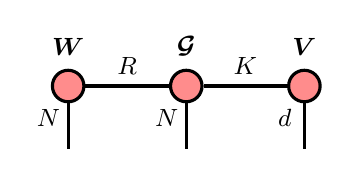
\begin{tikzpicture}

    \node[circle, line width = 0.4mm, draw = black, fill = red!45, inner sep = 0pt, minimum size = 0.4cm] (w) at (0, 0) {};
    \node at (0, 0.5) {\small{$\boldsymbol{W}$}};

    \node[circle, line width = 0.4mm, draw = black, fill = red!45, inner sep = 0pt, minimum size = 0.4cm] (g) at (1.5, 0) {};
    \node at (1.5, 0.5) {\small{$\boldsymbol{\mathcal{G}}$}};

    \node[circle, line width = 0.4mm, draw = black, fill = red!45, inner sep = 0pt, minimum size = 0.4cm] (v) at (3, 0) {};
    \node at (3, 0.5) {\small{$\boldsymbol{V}$}};

    \path [draw, line width = 0.4mm, -] (w) edge (g);
    \node at (0.75, 0.25) {\small{$R$}};
    \path [draw, line width = 0.4mm, -] (g) edge (v);
    \node at (2.25, 0.25) {\small{$K$}};

    \draw [line width = 0.4mm] (w) -- (0, -0.8);
    \node at (-0.25, -0.4) {\small{$N$}};
    \draw [line width = 0.4mm] (g) -- (1.5, -0.8);
    \node at (1.5-0.25, -0.4) {\small{$N$}};
    \draw [line width = 0.4mm] (v) -- (3, -0.8);
    \node at (3-0.25, -0.4) {\small{$d$}};

    \end{tikzpicture}
    \end{document}
\end{lstlisting}

编译后的绘制图形如图\ref{tik:2}所示。

\begin{figure}[h]
    \centering
    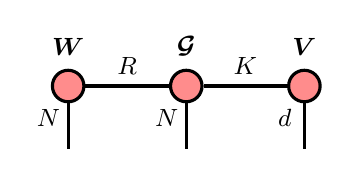
\begin{tikzpicture}
        \node[circle, line width = 0.4mm, draw = black, fill = red!45, inner sep = 0pt, minimum size = 0.4cm] (w) at (0, 0) {};
        \node at (0, 0.5) {\small{$\boldsymbol{W}$}};

        \node[circle, line width = 0.4mm, draw = black, fill = red!45, inner sep = 0pt, minimum size = 0.4cm] (g) at (1.5, 0) {};
        \node at (1.5, 0.5) {\small{$\boldsymbol{\mathcal{G}}$}};

        \node[circle, line width = 0.4mm, draw = black, fill = red!45, inner sep = 0pt, minimum size = 0.4cm] (v) at (3, 0) {};
        \node at (3, 0.5) {\small{$\boldsymbol{V}$}};

        \path [draw, line width = 0.4mm, -] (w) edge (g);
        \node at (0.75, 0.25) {\small{$R$}};
        \path [draw, line width = 0.4mm, -] (g) edge (v);
        \node at (2.25, 0.25) {\small{$K$}};

        \draw [line width = 0.4mm] (w) -- (0, -0.8);
        \node at (-0.25, -0.4) {\small{$N$}};
        \draw [line width = 0.4mm] (g) -- (1.5, -0.8);
        \node at (1.5-0.25, -0.4) {\small{$N$}};
        \draw [line width = 0.4mm] (v) -- (3, -0.8);
        \node at (3-0.25, -0.4) {\small{$d$}};
    \end{tikzpicture}
    \caption{绘制后的图形}
    \label{tik:2}
\end{figure}

\subsection{绘制直线}

我们在这两个示例中可以感受到TikZ功能的强大之处。但是,这些复杂的图形都是由最基本的点、线
和面所构成。在本小节中,我们将从绘制一条直线开始,入门这个强大的LaTeX绘图工具。首先,画
一条直线需要给出起始点坐标和终止点坐标,我们可以简单地通过如下代码:
\begin{lstlisting}[language=TeX]
    \begin{tikzpicture}
        \draw (x1,y1) -- (x2,y2); % 这里(x1,y1)和(x2,y2)在编译时均需替换成具体坐标数值。
    \end{tikzpicture}
\end{lstlisting}

来实现绘制一条从$(x1,y1)$到$(x2,y2)$的直线的功能。值得注意的是,在默认情况下,坐标系均以
cm为单位。

\emph{【例】}尝试绘制一条直线:
\begin{lstlisting}[language=TeX]
    \begin{tikzpicture}
        \draw (-2,0) -- (2,0);
    \end{tikzpicture}
\end{lstlisting}

进一步地,我们可以通过设定一系列的坐标点,来实现多条线段的连续绘制。

\emph{【例】}多条线段连续绘制:
\begin{lstlisting}[language=TeX]
    \begin{tikzpicture}
        \draw (-2,0) -- (2,0) -- (2,2) -- (-2,2) -- (-2,0);
    \end{tikzpicture}
\end{lstlisting}

也可以通过增加多行命令,实现多段线条的分开绘制。

\emph{【例】}多段线条分开绘制:
\begin{lstlisting}[language=TeX]
    \begin{tikzpicture}
        \draw (-2,0) -- (2,0) -- (2,2) -- (-2,2) -- (-2,0);
        \draw (0,4) -- (0,-2);
        \draw (3,-2) -- (3,4) -- (7,4) -- (7,-2) -- (3,-2);
        \draw (4,3) -- (6,3); \draw (4,1) -- (6,1); \draw (4,-1) -- (6,-1);
        \draw (5,3) -- (5,-1); \draw (5.75,0.25) -- (6.25,-0.25);
    \end{tikzpicture}    
\end{lstlisting}

编译后的绘制图形如图\ref{tik:3}所示。

\begin{figure}[h]
    \centering
    \begin{tikzpicture}

        \draw (-2,0) -- (2,0) -- (2,2) -- (-2,2) -- (-2,0);
        \draw (0,4) -- (0,-2);
        \draw (3,-2) -- (3,4) -- (7,4) -- (7,-2) -- (3,-2);
        \draw (4,3) -- (6,3); \draw (4,1) -- (6,1); \draw (4,-1) -- (6,-1);
        \draw (5,3) -- (5,-1); \draw (5.75,0.25) -- (6.25,-0.25);

    \end{tikzpicture}
    \caption{绘制后的图形}
    \label{tik:3}
\end{figure}

值得注意的是,在tikzpicture环境中,像\emph{Matlab}语言一样,我们需要采用\emph{;}符号来
标记一个指令的结束。这样的指令结束标记让我们不但可以在多行完成一条指令,同时也可以在一行
内实现多条指令。

\subsection{图形缩放}

在上小节中,我们绘制图形需要给出精确的坐标点。但是在绘制好之后,如果需要调整图形大小,我们
可以采用scale的方式对图形进行缩放。

\emph{【例】}整体缩放:
\begin{lstlisting}[language=TeX]
    \begin{tikzpicture}[scale=0.5]
        % 绘制内容
    \end{tikzpicture} 
\end{lstlisting}

\emph{【例】}横向缩放:
\begin{lstlisting}[language=TeX]
    \begin{tikzpicture}[xscale=1.5]
        % 绘制内容
    \end{tikzpicture} 
\end{lstlisting}

\emph{【例】}分别调整横向、纵向缩放:
\begin{lstlisting}[language=TeX]
    \begin{tikzpicture}[xscale=1.5, yscale = 2]
        % 绘制内容
    \end{tikzpicture} 
\end{lstlisting}

\subsection{绘制箭头}

在绘制直线的基础上,我们往往需要通过绘制箭头来指向性地表达意图。箭头的绘制只需要在直线绘制
的基础上,增加[option]进行声明即可。

\emph{【例】}绘制箭头:
\begin{lstlisting}[language=TeX]
    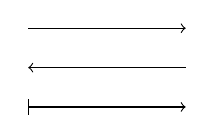
\begin{tikzpicture}

        \draw [->] (0,0) -- (2,0);
        \draw [<-] (0, -0.5) -- (2,-0.5);
        \draw [|->] (0,-1) -- (2,-1);
    
    \end{tikzpicture}
\end{lstlisting}

编译后的绘制图形如图\ref{tik:4}所示。

\begin{figure}[h]
    \centering
    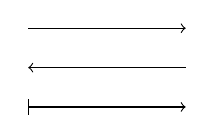
\begin{tikzpicture}

        \draw [->] (0,0) -- (2,0);
        \draw [<-] (0, -0.5) -- (2,-0.5);
        \draw [|->] (0,-1) -- (2,-1);

    \end{tikzpicture}
    \caption{绘制后的图形}
    \label{tik:4}
\end{figure}

\emph{【例】}利用绘制箭头的例子以及多条线段连续绘制的例子,用一行命令绘制一个直角坐标系:
\begin{lstlisting}[language=TeX]
    \begin{tikzpicture}

        \draw [<->] (0,2) -- (0,0) -- (3,0);
    
    \end{tikzpicture}
\end{lstlisting}

编译后的绘制图形如图\ref{tik:5}所示。

\begin{figure}[h]
    \centering
    \begin{tikzpicture}

        \draw [<->] (0,2) -- (0,0) -- (3,0);

    \end{tikzpicture}
    \caption{绘制后的图形}
    \label{tik:5}
\end{figure}

\subsection{调整线条粗细}

采用\texttt{\textbackslash{}draw}命令时,增加的[option]声明也可以用来调整线条的粗细。

\emph{【例】}绘制不同粗细的线条:
\begin{lstlisting}[language=TeX]
    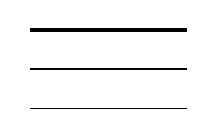
\begin{tikzpicture}

        \draw [ultra thick] (0,1) -- (2,1);
        \draw [thick] (0,0.5) -- (2,0.5);
        \draw [thin] (0,0) -- (2,0);
    
    \end{tikzpicture}
\end{lstlisting}

编译后的绘制图形如图\ref{tik:6}所示。

\begin{figure}[h]
    \centering
    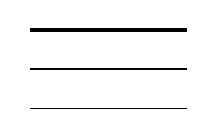
\begin{tikzpicture}

        \draw [ultra thick] (0,1) -- (2,1);
        \draw [thick] (0,0.5) -- (2,0.5);
        \draw [thin] (0,0) -- (2,0);

    \end{tikzpicture}
    \caption{绘制后的图形}
    \label{tik:6}
\end{figure}

其中,线条的粗细可以通过不同的指令来控制,从细到粗分别可调用:\emph{ultra thin},\emph{very thin},
\emph{thin},\emph{semithick},\emph{thick},\emph{very thick},\emph{ultra thick}。

\emph{【例】}绘制上述七种不同粗细的线条:
\begin{lstlisting}[language=TeX]
    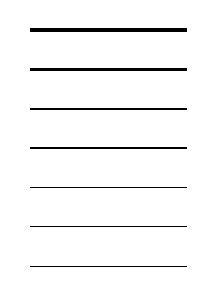
\begin{tikzpicture}

        \draw [ultra thin] (0,0) -- (2,0);
        \draw [very thin] (0,0.5) -- (2,0.5);
        \draw [thin] (0,1) -- (2,1);
        \draw [semithick] (0,1.5) -- (2,1.5);
        \draw [thick] (0,2) -- (2,2);
        \draw [very thick] (0,2.5) -- (2,2.5);
        \draw [ultra thick] (0,3) -- (2,3);
    
    \end{tikzpicture}
\end{lstlisting}

编译后的绘制图形如图\ref{tik:7}所示。

\begin{figure}[h]
    \centering
    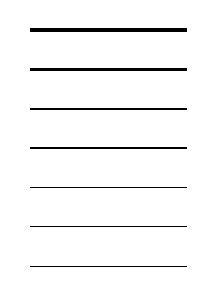
\begin{tikzpicture}

        \draw [ultra thin] (0,0) -- (2,0);
        \draw [very thin] (0,0.5) -- (2,0.5);
        \draw [thin] (0,1) -- (2,1);
        \draw [semithick] (0,1.5) -- (2,1.5);
        \draw [thick] (0,2) -- (2,2);
        \draw [very thick] (0,2.5) -- (2,2.5);
        \draw [ultra thick] (0,3) -- (2,3);

    \end{tikzpicture}
    \caption{绘制后的图形}
    \label{tik:7}
\end{figure}

除此之外,我们也可以自行定义线条的粗细,如[line width=5]、[line width=0.2cm]。值得注意
的是,当我们直接声明数值而不声明单位时,其默认单位均为pt。

\emph{【例】}使用line width参数绘制不同粗细线条:
\begin{lstlisting}[language=TeX]
    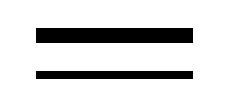
\begin{tikzpicture}
        \draw [line width=3] (0,0) -- (2,0);
        \draw [line width=0.2cm] (0,0.5) -- (2,0.5);
    \end{tikzpicture}
\end{lstlisting}

编译后的绘制图形如图\ref{tik:8}所示。

\begin{figure}[h]
    \centering
    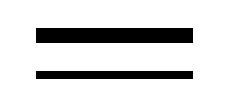
\begin{tikzpicture}

        \draw [line width=3] (0,0) -- (2,0);
        \draw [line width=0.2cm] (0,0.5) -- (2,0.5);

    \end{tikzpicture}
    \caption{绘制后的图形}
    \label{tik:8}
\end{figure}

\subsection{虚线}

我们也可以在[option]声明中增加对于线条形状的定义。如虚线\emph{dashed}和点线\emph{dotted}。

\emph{【例】}绘制虚线:
\begin{lstlisting}[language=TeX]
    \begin{tikzpicture}

        \draw [dashed, ultra thick] (0,1) -- (2,1); %我们可以通过组合多种option来声明线条的多种特征。
        \draw [dashed] (0, 0.5) -- (2,0.5);
        \draw [dotted] (0,0) -- (2,0);
    
    \end{tikzpicture}
\end{lstlisting}

编译后的绘制图形如图\ref{tik:9}所示。

\begin{figure}[h]
    \centering
    \begin{tikzpicture}

        \draw [dashed, ultra thick] (0,1) -- (2,1); %我们可以通过组合多种option来声明线条的多种特征。
        \draw [dashed] (0, 0.5) -- (2,0.5);
        \draw [dotted] (0,0) -- (2,0);

    \end{tikzpicture}
    \caption{绘制后的图形}
    \label{tik:9}
\end{figure}

\subsection{颜色}

我们也可以在[option]声明中增加对于线条颜色的定义。如红色\emph{red}、 绿色\emph{green}、蓝色\emph{blue}等等。

\emph{【例】}绘制不同颜色的直线:
\begin{lstlisting}[language=TeX]
    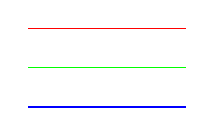
\begin{tikzpicture}

        \draw [red] (0,1) -- (2,1);
        \draw [green] (0, 0.5) -- (2,0.5);
        \draw [blue] (0,0) -- (2,0);
    
    \end{tikzpicture}
\end{lstlisting}

编译后的绘制图形如图\ref{tik:10}所示。

\begin{figure}[h]
    \centering
    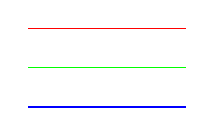
\begin{tikzpicture}

        \draw [red] (0,1) -- (2,1);
        \draw [green] (0, 0.5) -- (2,0.5);
        \draw [blue] (0,0) -- (2,0);

    \end{tikzpicture}
    \caption{绘制后的图形}
    \label{tik:10}
\end{figure}

\section{节点介绍}

节点是TikZ中的一个常用功能。在绘制节点时,通常需要声明其位置和形状,部分节点可以在其中添
加文字,同时也可以为节点赋予一个名称,用于后续参考。在本节中,我们将详细介绍节点的相关功
能及其应用。

\subsection{节点基本介绍}

\emph{【例】}绘制节点,方法一:
\begin{lstlisting}[language=TeX]
    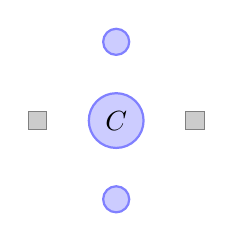
\begin{tikzpicture}
        \path (0,2) node [shape=circle,draw=blue!50,fill=blue!20,thick] {}
              (0,1) node [shape=circle,draw=blue!50,fill=blue!20,thick] {$C$}
              (0,0) node [shape=circle,draw=blue!50,fill=blue!20,thick] {}
              (1,1) node [shape=rectangle,draw=black!50,fill=black!20] {}
              (-1,1) node [shape=rectangle,draw=black!50,fill=black!20] {};
    \end{tikzpicture}
\end{lstlisting}

等价于

\emph{【例】}绘制节点,方法二:
\begin{lstlisting}[language=TeX]
    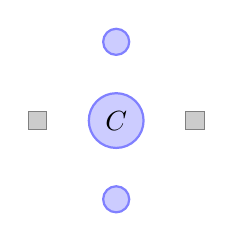
\begin{tikzpicture}
        \node [shape=circle,draw=blue!50,fill=blue!20,thick] at (0,2)  {};
        \node [shape=circle,draw=blue!50,fill=blue!20,thick] at (0,1) {$C$};
        \node [shape=circle,draw=blue!50,fill=blue!20,thick] at (0,0)  {};
        \node [shape=rectangle,draw=black!50,fill=black!20] at (1,1) {};
        \node [shape=rectangle,draw=black!50,fill=black!20] at (-1,1) {};
    \end{tikzpicture}
\end{lstlisting}

编译后的绘制图形如图\ref{tik:11}所示。

\begin{figure}[h]
    \centering
    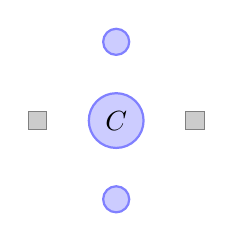
\begin{tikzpicture}

        \node [shape=circle,draw=blue!50,fill=blue!20,thick] at (0,2)  {};
        \node [shape=circle,draw=blue!50,fill=blue!20,thick] at (0,1) {$C$};
        \node [shape=circle,draw=blue!50,fill=blue!20,thick] at (0,0)  {};
        \node [shape=rectangle,draw=black!50,fill=black!20] at (1,1) {};
        \node [shape=rectangle,draw=black!50,fill=black!20] at (-1,1) {};

    \end{tikzpicture}
    \caption{绘制后的图形}
    \label{tik:11}
\end{figure}

这里需要注意的是,在[shape=circle,draw=blue!50,fill=blue!20]中,shape指令声明节点形状,
draw指令声明是否显现该形状的边框,并用draw=来声明边框颜色,fill命令指明该节点是否要填充,
并用fill=来声明填充颜色。若要在节点中显示文字,需在后面\{\}中填写对应的文字即可。

\subsection{节点样式}

当某一种形状及颜色的节点需要在不同位置多次出现时,上述代码显得不够优美。我们可以通过一段
代码提前声明该节点的样式,并反复调用这段代码即可。

\emph{【例】}绘制节点,方法三:
\begin{lstlisting}[language=TeX]
    \tikzstyle{aaa}=[circle,draw=blue!50,fill=blue!20,thick]
    \tikzstyle{bbb}=[rectangle,draw=black!50,fill=black!20]
    \begin{tikzpicture}

        \path (0,2) node [aaa] {}
            (0,1) node [aaa] {$C$}
            (0,0) node [aaa] {}
            (1,1) node [bbb] {}
            (-1,1) node [bbb] {};

    \end{tikzpicture}
\end{lstlisting}

编译上述代码,得到图形与图\ref{tik:11}所示相同。

\subsection{节点命名}

为了将节点相互连接起来,我们需要指明连接哪两个节点。因此,每个节点需要我们声明一个名称。
声明名称有两种方式,一种是采用name=的方式,另一种是在\texttt{\textbackslash{}node}后
用括号声明。

\emph{【例】}绘制节点,并声明节点名称,方法一:
\begin{lstlisting}[language=TeX]
    \tikzstyle{aaa}=[circle,draw=blue!50,fill=blue!20,thick]
    \tikzstyle{bbb}=[rectangle,draw=black!50,fill=black!20]
    \begin{tikzpicture}

        \path (0,2) node [aaa,name=a1] {}
            (0,1) node [aaa,name=a2] {$C$}
            (0,0) node [aaa,name=a3] {}
            (1,1) node [bbb,name=b1] {}
            (-1,1) node [bbb,name=b2] {};

    \end{tikzpicture}
\end{lstlisting}

\emph{【例】}绘制节点,并声明节点名称,方法二:
\begin{lstlisting}[language=TeX]
    \tikzstyle{aaa}=[circle,draw=blue!50,fill=blue!20,thick]
    \tikzstyle{bbb}=[rectangle,draw=black!50,fill=black!20]
    \begin{tikzpicture}

        \node (a1) [aaa] at (0,2)  {};
        \node (a2) [aaa] at (0,1) {$C$};
        \node (a3) [aaa] at (0,0)  {};
        \node (b1) [bbb] at (1,1) {};
        \node (b2) [bbb] at (-1,1) {};

    \end{tikzpicture}
\end{lstlisting}

\subsection{基于相对位置绘制节点}

给每个节点命名后,我们便可以通过above of(上)、below of(下)、left of(左)、right of(右)
等命令来声明新节点与某个节点的相对位置来绘制图形。

\emph{【例】}利用相对位置绘制节点:
\begin{lstlisting}[language=TeX]
    \tikzstyle{aaa}=[circle,draw=blue!50,fill=blue!20,thick]
    \tikzstyle{bbb}=[rectangle,draw=black!50,fill=black!20]
    \begin{tikzpicture}

        \node (a1) [aaa]                {};
        \node (a2) [aaa]  [below of=a1] {$C$};
        \node (a3) [aaa]  [below of=a2] {};
        \node (b1) [bbb]  [right of=a2] {};
        \node (b2) [bbb]  [left  of=a2] {};

    \end{tikzpicture}
\end{lstlisting}

编译上述代码,得到图形与图\ref{tik:11}所示相同。

\subsection{连接节点}

有了节点名称了,我们就可以对节点进行连接。我们拿连接A与B节点为例,在连接时,我们通常需要
声明A节点的哪个位置与B节点的哪个位置连接。位置声明通常采用east(右)、west(左)、north
(上)、south(下)、center(中心)等命令。

\emph{【例】}利用相对位置连接节点:
\begin{lstlisting}[language=TeX]
    \tikzstyle{aaa}=[circle,draw=blue!50,fill=blue!20,thick]
    \tikzstyle{bbb}=[rectangle,draw=black!50,fill=black!20]
    \begin{tikzpicture}

        \node (a1) [aaa]                {$a_1$};
        \node (a2) [aaa]  [below of=a1] {$C$};
        \node (a3) [aaa]  [below of=a2] {$a_3$};
        \node (b1) [bbb]  [right of=a2] {$b_1$};
        \node (b2) [bbb]  [left  of=a2] {$b_2$};
        \draw [->] (a2.west) -- (b2.east);
        \draw [->] (a2.east) -- (b1.west);
        \draw [->] (a2.north) -- (a1.south);
        \draw [->] (a2.south) -- (a3.north);

    \end{tikzpicture}
\end{lstlisting}

该代码等价于

\emph{【例】}利用相对位置连接节点,不声明节点的连接位置:
\begin{lstlisting}[language=TeX]
    \tikzstyle{aaa}=[circle,draw=blue!50,fill=blue!20,thick]
    \tikzstyle{bbb}=[rectangle,draw=black!50,fill=black!20]
    \begin{tikzpicture}

        \node (a1) [aaa]                {$a_1$};
        \node (a2) [aaa]  [below of=a1] {$C$};
        \node (a3) [aaa]  [below of=a2] {$a_3$};
        \node (b1) [bbb]  [right of=a2] {$b_1$};
        \node (b2) [bbb]  [left  of=a2] {$b_2$};
        \draw [->] (a2) -- (b2);
        \draw [->] (a2) -- (b1);
        \draw [->] (a2) -- (a1);
        \draw [->] (a2) -- (a3);

    \end{tikzpicture}
\end{lstlisting}

编译后的绘制图形如图\ref{tik:12}所示。

\begin{figure}[h]
    \centering
    \tikzstyle{aaa}=[circle,draw=blue!50,fill=blue!20,thick]
    \tikzstyle{bbb}=[rectangle,draw=black!50,fill=black!20]
    \begin{tikzpicture}

        \node (a1) [aaa]                {$a_1$};
        \node (a2) [aaa]  [below of=a1] {$C$};
        \node (a3) [aaa]  [below of=a2] {$a_3$};
        \node (b1) [bbb]  [right of=a2] {$b_1$};
        \node (b2) [bbb]  [left  of=a2] {$b_2$};
        \draw [->] (a2) -- (b2);
        \draw [->] (a2) -- (b1);
        \draw [->] (a2) -- (a1);
        \draw [->] (a2) -- (a3);

    \end{tikzpicture}
    \caption{绘制后的图形}
    \label{tik:12}
\end{figure}

\emph{【例】}利用edge命令连接节点,方法一:
\begin{lstlisting}[language=TeX]
    \tikzstyle{aaa}=[circle,draw=blue!50,fill=blue!20,thick]
    \tikzstyle{bbb}=[rectangle,draw=black!50,fill=black!20]
    \begin{tikzpicture}

        \node (a1) [aaa]                {$a_1$};
        \node (a2) [aaa]  [below of=a1] {$C$}   edge [->] (a1);
        \node (a3) [aaa]  [below of=a2] {$a_3$} edge [<-] (a2);
        \node (b1) [bbb]  [right of=a2] {$b_1$} edge [<-] (a2);
        \node (b2) [bbb]  [left  of=a2] {$b_2$} edge [<-] (a2);

    \end{tikzpicture}
\end{lstlisting}

等价于

\emph{【例】}用edge命令连接节点,方法二:
\begin{lstlisting}[language=TeX]
    \tikzstyle{aaa}=[circle,draw=blue!50,fill=blue!20,thick]
    \tikzstyle{bbb}=[rectangle,draw=black!50,fill=black!20]
    \begin{tikzpicture}

        \path (0,2)  node [aaa,name=a1] {$a_1$}
            (0,1)  node [aaa,name=a2] {$C$}   edge [->] (a1)
            (0,0)  node [aaa,name=a3] {$a_3$} edge [<-] (a2)
            (1,1)  node [bbb,name=b1] {$b_1$} edge [<-] (a2)
            (-1,1) node [bbb,name=b2] {$b_2$} edge [<-] (a2);

    \end{tikzpicture}
\end{lstlisting}

编译上述代码,得到图形与图\ref{tik:12}所示相同。

\emph{【例】}声明每个节点的连接位置,将周围节点边缘连接直中间节点的中心:
\begin{lstlisting}[language=TeX]
    \tikzstyle{aaa}=[circle,draw=blue!50,fill=blue!20,thick]
    \tikzstyle{bbb}=[rectangle,draw=black!50,fill=black!20]
    \begin{tikzpicture}

        \node (a1) [aaa]                {$a_1$};
        \node (a2) [aaa]  [below of=a1] {};
        \node (a3) [aaa]  [below of=a2] {$a_3$};
        \node (b1) [bbb]  [right of=a2] {$b_1$};
        \node (b2) [bbb]  [left  of=a2] {$b_2$};
        \draw [->] (a2.center) -- (b2.east);
        \draw [->] (a2.center) -- (b1.west);
        \draw [->] (a2.center) -- (a1.south);
        \draw [->] (a2.center) -- (a3.north);

    \end{tikzpicture}
\end{lstlisting}

编译上述代码,得到图形如图\ref{tik:13}所示。

\begin{figure}[h]
    \centering
    \tikzstyle{aaa}=[circle,draw=blue!50,fill=blue!20,thick]
    \tikzstyle{bbb}=[rectangle,draw=black!50,fill=black!20]
    \begin{tikzpicture}

        \node (a1) [aaa]                {$a_1$};
        \node (a2) [aaa]  [below of=a1] {};
        \node (a3) [aaa]  [below of=a2] {$a_3$};
        \node (b1) [bbb]  [right of=a2] {$b_1$};
        \node (b2) [bbb]  [left  of=a2] {$b_2$};
        \draw [->] (a2.center) -- (b2.east);
        \draw [->] (a2.center) -- (b1.west);
        \draw [->] (a2.center) -- (a1.south);
        \draw [->] (a2.center) -- (a3.north);

    \end{tikzpicture}
    \caption{绘制后的图形}
    \label{tik:13}
\end{figure}

\section{高级功能}

在本节中,我们将介绍除直线以外的复杂功能,如:非规则曲线、复杂函数绘图、区域填充、填写标签等等。

\subsection{矩形、圆形、曲线}

我们可以通过\texttt{\textbackslash{}draw (x,y) rectangle (w,h);}的方式绘制一个矩形,
其左下角坐标位于点$(x,y)$处,长度为$𝑤$,高度为$ℎ$。类似地,我们也可以通过\texttt{\textbackslash{}draw (x,y) circle [radius=r];}的方式绘制一个圆形,其圆心落在点$(x,y)$处,半径为$𝑟$。除此之外,我们可以通过
\texttt{\textbackslash{}draw (x,y) arc [radius=r, start angle=a1, end angle=a2]}
的方式绘制一条弧线,它从点$(x,y)$处开始绘制,该弧线曲率半径为$𝑟$,其起始角度为所对应曲
率圆的$𝑎1$处,终止角度为所对应曲率圆的$𝑎2$处。

\emph{【例】}按上述介绍,绘制矩形、圆形以曲线:
\begin{lstlisting}[language=TeX]
    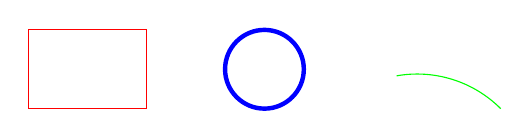
\begin{tikzpicture}

        \draw [red] (0,0) rectangle (1.5,1);
        \draw [blue, ultra thick] (3,0.5) circle [radius=0.5];
        \draw [green] (6,0) arc [radius=1.5, start angle=45, end angle= 100];
    
    \end{tikzpicture}
\end{lstlisting}

编译上述代码,得到图形如图\ref{tik:14}所示。

\begin{figure}[h]
    \centering
    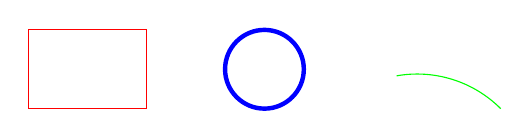
\begin{tikzpicture}

        \draw [red] (0,0) rectangle (1.5,1);
        \draw [blue, ultra thick] (3,0.5) circle [radius=0.5];
        \draw [green] (6,0) arc [radius=1.5, start angle=45, end angle= 100];

    \end{tikzpicture}
    \caption{绘制后的图形}
    \label{tik:14}
\end{figure}

\subsection{平滑过渡曲线}

在绘图时,一种不突兀地连接两条直线的方式是采用平滑过渡圆角/曲线。在本节中,我们将介绍两种
平滑过渡曲线的绘制方法:绘制带圆角的曲线和绘制过渡曲线。

\emph{【例】}绘制带圆角的坐标系:
\begin{lstlisting}[language=TeX]
    \begin{tikzpicture}

        \draw [<->, rounded corners, thick, purple] (0,2) -- (0,0) -- (3,0);
    
    \end{tikzpicture}
\end{lstlisting}

编译上述代码,得到图形如图\ref{tik:15}所示。

\begin{figure}[h]
    \centering
    \begin{tikzpicture}

        \draw [<->, rounded corners, thick, purple] (0,2) -- (0,0) -- (3,0);

    \end{tikzpicture}
    \caption{绘制后的图形}
    \label{tik:15}
\end{figure}

\emph{【例】}绘制过渡曲线:
\begin{lstlisting}[language=TeX]
    \begin{tikzpicture}

        \draw[<-, thick] (0,2) -- (0,0.5);
        \draw[thick,red] (0,0.5) to [out=270,in=180] (0.5,0);
        \draw[->, thick] (0.5,0) -- (3,0);
    
    \end{tikzpicture}
\end{lstlisting}

编译上述代码,得到图形如图\ref{tik:16}所示。

\begin{figure}[h]
    \centering
    \begin{tikzpicture}

        \draw[<-, thick] (0,2) -- (0,0.5);
        \draw[thick,red] (0,0.5) to [out=270,in=180] (0.5,0);
        \draw[->, thick] (0.5,0) -- (3,0);

    \end{tikzpicture}
    \caption{绘制后的图形}
    \label{tik:16}
\end{figure}

\emph{【例】}利用多段过渡曲线绘制S曲线:
\begin{lstlisting}[language=TeX]
    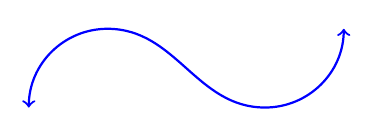
\begin{tikzpicture}

        \draw [<->,thick, blue] (0,0) to [out=90,in=180] (1,1) to [out=0,in=180] (3,0) to [out=0,in=-90] (4,1) ;
    
    \end{tikzpicture}
\end{lstlisting}

编译上述代码,得到图形如图\ref{tik:17}所示。

\begin{figure}[h]
    \centering
    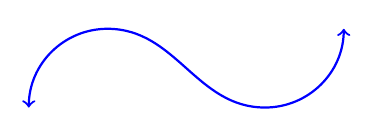
\begin{tikzpicture}

        \draw [<->,thick, blue] (0,0) to [out=90,in=180] (1,1) to [out=0,in=180] (3,0) to [out=0,in=-90] (4,1) ;

    \end{tikzpicture}
    \caption{绘制后的图形}
    \label{tik:17}
\end{figure}

\subsection{根据函数绘制曲线}

TikZ宏包的强大之处在于,它还提供了可供绘制函数的数学引擎。在此我们先给出一个示例,再详细
讲解如何利用该宏包绘制函数所对应的曲线。

\emph{【例】}利用函数绘制正弦曲线:
\begin{lstlisting}[language=TeX]
    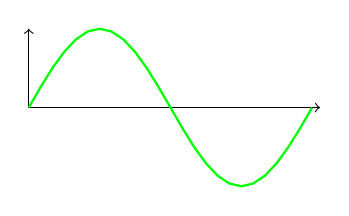
\begin{tikzpicture}[xscale=0.01,yscale=1]

        \draw [<->] (0,1) -- (0,0) -- (370,0);
        \draw[green, thick, domain=0:360] plot (\x, {sin(\x)}); % 这里需要注意带上{}
    
    \end{tikzpicture}
\end{lstlisting}

编译上述代码,得到图形如图\ref{tik:18}所示。

\begin{figure}[h]
    \centering
    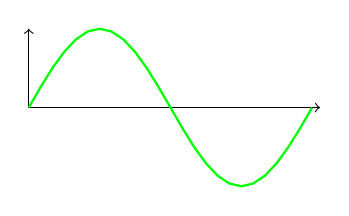
\begin{tikzpicture}[xscale=0.01,yscale=1]

        \draw [<->] (0,1) -- (0,0) -- (370,0);
        \draw[green, thick, domain=0:360] plot (\x, {sin(\x)}); % 这里需要注意带上{}

    \end{tikzpicture}
    \caption{绘制后的图形}
    \label{tik:18}
\end{figure}

在上述例子中,\emph{domain}指令声明了横坐标$x$的范围。在本示例中,我们利用\emph{sin}函
数绘制了一段正弦曲线。

除了本示例中的正弦曲线\emph{sin}函数,我们还可以调用大量其他函数,在此列举一部分作为示例:
\begin{itemize}
    \item 阶乘函数:\texttt{factorial(\textbackslash{}x)};
    \item 平方根函数:\texttt{sqrt(\textbackslash{}x)};
    \item 幂函数:\texttt{pow(\textbackslash{}x,y)};
    \item 指数函数:\texttt{exp(\textbackslash{}x)};
    \item 对数函数:\texttt{ln(\textbackslash{}x)}、\texttt{log10(\textbackslash{}x)}、\texttt{log2(\textbackslash{}x)};
    \item 绝对值函数:\texttt{abs(\textbackslash{}x)};
    \item 取余函数:\texttt{mod(\textbackslash{}x,y)}(即求$𝑥$被$𝑦$除后的余数);
    \item 圆整函数:\texttt{round(\textbackslash{}x)}、\texttt{floor(\textbackslash{}x)}、\texttt{ceil(\textbackslash{}x)};三角函数:\texttt{sin(\textbackslash{}x)}、\texttt{cos(\textbackslash{}x)}、\texttt{tan(\textbackslash{}x)}。
          ;
\end{itemize}

值得注意的是,在三角函数中,通常默认自变量$𝑥$以度(°)为单位。若要采用弧度制,则需要将函
数分别改写为\texttt{sin(\textbackslash{}x r)}、\texttt{cos(\textbackslash{}x r)}、\texttt{tan(\textbackslash{}x r)}。
除了这部分常用函数之外,我们通常还会使用两个常数$e$($𝑒=2.718281828$)和$pi$($𝑝𝑖=3.141592654$)。

通过组合以上基本函数,我们可以实现更复杂的函数功能。

\emph{【例】}利用函数绘制正弦曲线:
\begin{lstlisting}[language=TeX]
    \begin{tikzpicture}[yscale=1.5]

        \draw [thick, ->] (0,0) -- (6.5,0);
        \draw [thick, ->] (0,-1.1) -- (0,1.1);
        \draw [green,domain=0:2*pi] plot (\x, {(sin(\x r)* ln(\x+1))/2});
        \draw [red,domain=0:pi] plot (\x, {sin(\x r)});
        \draw [blue, domain=pi:2*pi] plot (\x, {cos(\x r)*exp(\x/exp(2*pi))});
    
    \end{tikzpicture}
\end{lstlisting}

编译上述代码,得到图形如图\ref{tik:19}所示。

\begin{figure}[h]
    \centering
    \begin{tikzpicture}[yscale=1.5]

        \draw [thick, ->] (0,0) -- (6.5,0);
        \draw [thick, ->] (0,-1.1) -- (0,1.1);
        \draw [green,domain=0:2*pi] plot (\x, {(sin(\x r)* ln(\x+1))/2});
        \draw [red,domain=0:pi] plot (\x, {sin(\x r)});
        \draw [blue, domain=pi:2*pi] plot (\x, {cos(\x r)*exp(\x/exp(2*pi))});

    \end{tikzpicture}
    \caption{绘制后的图形}
    \label{tik:19}
\end{figure}

\subsection{简单图形的区域填充}

我们可以在简单图形的基础上进行区域填充。

\emph{【例】}简单形状的区域填充:
\begin{lstlisting}[language=TeX]
    \begin{tikzpicture}[yscale=1.5]

        \draw [fill=red,ultra thick] (0,0) rectangle (1,1);
        \draw [fill=red,ultra thick,red] (2,0) rectangle (3,1); % 这里的第二个red声明了区域周围边框线的颜色
        \draw [blue, fill=blue] (4,0) -- (5,1) -- (4.75,0.15) -- (4,0);
        \draw [fill] (7,0.5) circle [radius=0.1];
        \draw [fill=orange] (9,0) rectangle (11,1);
        \draw [fill=white] (9.25,0.25) rectangle (10,1.5);
    
    \end{tikzpicture}
\end{lstlisting}

编译上述代码,得到图形如图\ref{tik:20}所示。

\begin{figure}[h]
    \centering
    \begin{tikzpicture}[yscale=1.5]

        \draw [fill=red,ultra thick] (0,0) rectangle (1,1);
        \draw [fill=red,ultra thick,red] (2,0) rectangle (3,1); % 这里的第二个red声明了区域周围边框线的颜色
        \draw [blue, fill=blue] (4,0) -- (5,1) -- (4.75,0.15) -- (4,0);
        \draw [fill] (7,0.5) circle [radius=0.1];
        \draw [fill=orange] (9,0) rectangle (11,1);
        \draw [fill=white] (9.25,0.25) rectangle (10,1.5);

    \end{tikzpicture}
    \caption{绘制后的图形}
    \label{tik:20}
\end{figure}

如上例中的注释所提,我们可以通过声明图形边框线的颜色来对边框线进行个性化更改。若并不希望
出现边框线,我们可以采用path命令替换\texttt{\textbackslash{}draw}命令。

\emph{【例】}简单形状的区域填充:
\begin{lstlisting}[language=TeX]
    \begin{tikzpicture}[yscale=1.5]

        \path [fill=red,thick] (0,0) rectangle (1.5,1);
        \draw [fill=red,thick] (2,0) rectangle (3.5,1);
    
    \end{tikzpicture}
\end{lstlisting}

编译上述代码,得到图形如图\ref{tik:21}所示。

\begin{figure}[h]
    \centering
    \begin{tikzpicture}[yscale=1.5]

        \path [fill=red,thick] (0,0) rectangle (1.5,1);
        \draw [fill=red,thick] (2,0) rectangle (3.5,1);

    \end{tikzpicture}
    \caption{绘制后的图形}
    \label{tik:21}
\end{figure}

\subsection{在图形中填写标签}

在绘图时,在合适的位置加入适当的文字进行说明,对内容的表达具有很重要的作用。在本节中,我们
将通过\texttt{\textbackslash{}node}来实现这一功能。

\emph{【例】}在直角坐标系中插入文字:
\begin{lstlisting}[language=TeX]
    \begin{tikzpicture}[yscale=1.5]

        \draw [thick, <->] (0,2) -- (0,0) -- (2,0);
        \node at (1,1) {good};
    
    \end{tikzpicture}
\end{lstlisting}

编译上述代码,得到图形如图\ref{tik:22}所示。

\begin{figure}[h]
    \centering
    \begin{tikzpicture}[yscale=1.5]

        \draw [thick, <->] (0,2) -- (0,0) -- (2,0);
        \node at (1,1) {good};

    \end{tikzpicture}
    \caption{绘制后的图形}
    \label{tik:22}
\end{figure}

在上例中,我们给出了一个简单的示范,我们将文字"good"的中心位置固定在坐标(1,1)点处。当然,
我们也可以通过命令,控制文字与所声明坐标的相对位置,如:在坐标上方、下方、左侧、右侧。

\emph{【例】}在(1,1)点下方插入文字:
\begin{lstlisting}[language=TeX]
    \begin{tikzpicture}

        \draw [thick, <->] (0,2) -- (0,0) -- (2,0);
        \draw [fill] (1,1) circle [radius=0.025];
        \node [below] at (1,1) {good};
    
    \end{tikzpicture}
\end{lstlisting}

编译上述代码,得到图形如图\ref{tik:23}所示。

\begin{figure}[h]
    \centering
    \begin{tikzpicture}

        \draw [thick, <->] (0,2) -- (0,0) -- (2,0);
        \draw [fill] (1,1) circle [radius=0.025];
        \node [below] at (1,1) {good};

    \end{tikzpicture}
    \caption{绘制后的图形}
    \label{tik:23}
\end{figure}

\emph{【例】}在(1,1)点上方、下方、左侧、右侧插入文字:
\begin{lstlisting}[language=TeX]
    \begin{tikzpicture}

        \draw [thick, <->] (0,2) -- (0,0) -- (2,0);
        \draw [fill] (1,1) circle [radius=0.025];
        \node [below] at (1,1) {below};
        \node [above] at (1,1) {above};
        \node [left] at (1,1) {left};
        \node [right] at (1,1) {right};
    
    \end{tikzpicture}
\end{lstlisting}

编译上述代码,得到图形如图\ref{tik:24}所示。

\begin{figure}[h]
    \centering
    \begin{tikzpicture}

        \draw [thick, <->] (0,2) -- (0,0) -- (2,0);
        \draw [fill] (1,1) circle [radius=0.025];
        \node [below] at (1,1) {below};
        \node [above] at (1,1) {above};
        \node [left] at (1,1) {left};
        \node [right] at (1,1) {right};

    \end{tikzpicture}
    \caption{绘制后的图形}
    \label{tik:24}
\end{figure}

\emph{【例】}在(1,1)点处插入数学符号$\theta$:
\begin{lstlisting}[language=TeX]
    \begin{tikzpicture}

        \draw [thick, <->] (0,2) -- (0,0) -- (2,0);
        \node [below right] at (2,0) {$x$};
        \node [left] at (0,2) {$y$};
        \draw[fill] (1,1) circle [radius=.5pt];
        \node[above right] at (1,1) {$\theta$};
    
    \end{tikzpicture}
\end{lstlisting}

编译上述代码,得到图形如图\ref{tik:25}所示。

\begin{figure}[h]
    \centering
    \begin{tikzpicture}

        \draw [thick, <->] (0,2) -- (0,0) -- (2,0);
        \node [below right] at (2,0) {$x$};
        \node [left] at (0,2) {$y$};
        \draw[fill] (1,1) circle [radius=.5pt];
        \node[above right] at (1,1) {$\theta$};

    \end{tikzpicture}
    \caption{绘制后的图形}
    \label{tik:25}
\end{figure}

\section{复杂模型实战解析}

在本节中,我们将给出一些科研论文中的复杂模型供读者们进一步解析学习。

\emph{【例】}BCPF:
\begin{lstlisting}[language=TeX]
    \documentclass[border=0.1cm]{standalone}
    \usepackage[utf8]{inputenc}

    \usepackage{tikz}
    \usepackage{amsfonts}
    \usepackage{amsmath,amssymb}
    \usepackage{systeme,mathtools}
    \usetikzlibrary{positioning,arrows.meta,quotes}
    \usetikzlibrary{shapes,snakes}
    \usetikzlibrary{bayesnet}
    \tikzset{>=latex}
    \tikzstyle{plate caption} = [caption, node distance=0, inner sep=0pt,
    below left=5pt and 0pt of #1.south]

    \begin{document}
    \begin{tikzpicture}

        \node [obs] (x) at (0,0) {\large $x_{\boldsymbol{i}}$};
        \node [circle,draw=black,fill=white,inner sep=0pt,minimum size=0.6cm] (u1) at (-1.2,1.6) { $\boldsymbol{u}_{i_1}^{(1)}$};
        \node [circle,draw=black,fill=white,inner sep=0pt,minimum size=0.6cm] (u3) at (1.2,1.6) { $\boldsymbol{u}_{i_d}^{(d)}$};
        \node [circle,draw=black,fill=white,inner sep=0pt,minimum size=0.65cm] (lambda) at (0,3.0) {\large $\boldsymbol{\lambda}$};

        \node[mark size=1pt,color=black] at (0,1.6) {\pgfuseplotmark{*}};
        \node[mark size=1pt,color=black] at (-0.2,1.6) {\pgfuseplotmark{*}};
        \node[mark size=1pt,color=black] at (0.2,1.6) {\pgfuseplotmark{*}};

        \node [text width=0.5cm] (c0) at (0,4) {$\alpha,\beta$};
        \node [text width=0.5cm] (a0) at (2.5,2.6) {$\alpha,\beta$};
        \node [circle,draw=black,fill=white,inner sep=0pt,minimum size=0.65cm] (tau_epsilon) at (2.5,1.6) {\large $\tau_{\epsilon}$};

        \path [draw,->] (u1) edge (x);
        \path [draw,->] (u3) edge (x);
        \path [draw,->] (lambda) edge (u1);
        \path [draw,->] (lambda) edge (u3);

        \path [draw,->] (c0) edge (lambda);
        \path [draw,->] (tau_epsilon) edge (x);
        \path [draw,->] (a0) edge (tau_epsilon);
        \plate [color=red] {part1} {(x)(u1)} { };
        \plate [color=blue] {part3} {(x)(u3)(part1.north east)} { };

        \node [text width=2cm] at (-0.6,-0.5) {\large $n_1$};
        \node [text width=2cm] at (2,-0.5) {\large $n_d$};

    \end{tikzpicture}
    \end{document}
\end{lstlisting}

编译上述代码,得到图形如图\ref{tik:26}所示。

\begin{figure}[h]
    \centering
    \usetikzlibrary{positioning,arrows.meta,quotes}
    \usetikzlibrary{shapes,snakes}
    \usetikzlibrary{bayesnet}
    \tikzset{>=latex}
    \tikzstyle{plate caption} = [caption, node distance=0, inner sep=0pt,
    below left=5pt and 0pt of #1.south]

    \begin{tikzpicture}

        \node [obs] (x) at (0,0) {\large $x_{\boldsymbol{i}}$};
        \node [circle,draw=black,fill=white,inner sep=0pt,minimum size=0.6cm] (u1) at (-1.2,1.6) { $\boldsymbol{u}_{i_1}^{(1)}$};
        \node [circle,draw=black,fill=white,inner sep=0pt,minimum size=0.6cm] (u3) at (1.2,1.6) { $\boldsymbol{u}_{i_d}^{(d)}$};
        \node [circle,draw=black,fill=white,inner sep=0pt,minimum size=0.65cm] (lambda) at (0,3.0) {\large $\boldsymbol{\lambda}$};

        \node[mark size=1pt,color=black] at (0,1.6) {\pgfuseplotmark{*}};
        \node[mark size=1pt,color=black] at (-0.2,1.6) {\pgfuseplotmark{*}};
        \node[mark size=1pt,color=black] at (0.2,1.6) {\pgfuseplotmark{*}};

        \node [text width=0.5cm] (c0) at (0,4) {$\alpha,\beta$};
        \node [text width=0.5cm] (a0) at (2.5,2.6) {$\alpha,\beta$};
        \node [circle,draw=black,fill=white,inner sep=0pt,minimum size=0.65cm] (tau_epsilon) at (2.5,1.6) {\large $\tau_{\epsilon}$};

        \path [draw,->] (u1) edge (x);
        \path [draw,->] (u3) edge (x);
        \path [draw,->] (lambda) edge (u1);
        \path [draw,->] (lambda) edge (u3);

        \path [draw,->] (c0) edge (lambda);
        \path [draw,->] (tau_epsilon) edge (x);
        \path [draw,->] (a0) edge (tau_epsilon);
        \plate [color=red] {part1} {(x)(u1)} { };
        \plate [color=blue] {part3} {(x)(u3)(part1.north east)} { };

        \node [text width=2cm] at (-0.6,-0.5) {\large $n_1$};
        \node [text width=2cm] at (2,-0.5) {\large $n_d$};

    \end{tikzpicture}
    \caption{绘制后的图形}
    \label{tik:26}
\end{figure}

\emph{【例】}矩阵分解示意图:
\begin{lstlisting}[language=TeX]
    \documentclass[border=0.1cm]{standalone}
    \usepackage[utf8]{inputenc}

    \usepackage{tikz}
    \usepackage{amsfonts}
    \usepackage{amsmath,amssymb}
    \usepackage{systeme,mathtools}
    \usetikzlibrary{positioning,arrows.meta,quotes}
    \usetikzlibrary{shapes,snakes}
    \usetikzlibrary{bayesnet}
    \tikzset{>=latex}

    \begin{document}
    \begin{tikzpicture}

        \draw [very thick] (0,0) rectangle (3.6/2,2.4/2);
        \filldraw [fill=green!20!white,draw=green!40!black] (0,0) rectangle (3.6/2,2.4/2);
        \filldraw [fill=white] (0.4/2,0.4/2) rectangle (0.8/2,0.8/2);
        \filldraw [fill=white] (2.4/2,0.4/2) rectangle (2.8/2,0.8/2);
        \filldraw [fill=white] (0.8/2,1.2/2) rectangle (1.2/2,1.6/2);
        \filldraw [fill=white] (2.0/2,1.6/2) rectangle (2.4/2,2.0/2);
        \filldraw [fill=white] (0.4/2,2.0/2) rectangle (0.8/2,2.4/2);
        \filldraw [fill=white] (2.4/2,2.0/2) rectangle (2.8/2,2.4/2);
        \filldraw [fill=white] (2.8/2,1.2/2) rectangle (3.2/2,2.0/2);
        \draw [step=0.4/2, very thin, color=gray] (0,0) grid (3.6/2,2.4/2);
        \draw (1.8/2,-0.3) node {{\color{red}\scriptsize{$Y\in\mathbb{R}^{m\times f}$}}};
        \draw (4.4/2,1.2/2) node {{\color{black}\large{$\approx$}}};
        \draw [very thick] (5.2/2,0) rectangle (6.0/2,2.4/2);
        \filldraw [fill=green!20!white,draw=green!40!black] (5.2/2,0) rectangle (6.0/2,2.4/2);
        \draw [step=0.4/2, very thin, color=gray] (5.2/2,0) grid (6.0/2,2.4/2);
        \draw (5.6/2,-0.3) node {{\color{black}\scriptsize{$W\in\mathbb{R}^{m\times r}$}}};
        \draw (6.8/2,1.2/2) node {{\color{black}\large{$\times$}}};
        \draw [very thick] (7.6/2,0.8/2) rectangle (11.2/2,1.6/2);
        \filldraw [fill=green!20!white,draw=green!40!black] (7.6/2,0.8/2) rectangle (11.2/2,1.6/2);
        \draw [step=0.4/2, very thin, color=gray] (7.6/2,0.8/2) grid (11.2/2,1.6/2);
        \draw (9.4/2,0) node {{\color{red}\scriptsize{$X^{T}\in\mathbb{R}^{r\times f}$}}};

    \end{tikzpicture}
    \end{document}
\end{lstlisting}

编译上述代码,得到图形如图\ref{tik:28}所示。

\begin{figure}[h]
    \centering
    \usetikzlibrary{positioning,arrows.meta,quotes}
    \usetikzlibrary{shapes,snakes}
    \usetikzlibrary{bayesnet}
    \tikzset{>=latex}

    \begin{tikzpicture}

        \draw [very thick] (0,0) rectangle (3.6/2,2.4/2);
        \filldraw [fill=green!20!white,draw=green!40!black] (0,0) rectangle (3.6/2,2.4/2);
        \filldraw [fill=white] (0.4/2,0.4/2) rectangle (0.8/2,0.8/2);
        \filldraw [fill=white] (2.4/2,0.4/2) rectangle (2.8/2,0.8/2);
        \filldraw [fill=white] (0.8/2,1.2/2) rectangle (1.2/2,1.6/2);
        \filldraw [fill=white] (2.0/2,1.6/2) rectangle (2.4/2,2.0/2);
        \filldraw [fill=white] (0.4/2,2.0/2) rectangle (0.8/2,2.4/2);
        \filldraw [fill=white] (2.4/2,2.0/2) rectangle (2.8/2,2.4/2);
        \filldraw [fill=white] (2.8/2,1.2/2) rectangle (3.2/2,2.0/2);
        \draw [step=0.4/2, very thin, color=gray] (0,0) grid (3.6/2,2.4/2);
        \draw (1.8/2,-0.3) node {{\color{red}\scriptsize{$Y\in\mathbb{R}^{m\times f}$}}};
        \draw (4.4/2,1.2/2) node {{\color{black}\large{$\approx$}}};
        \draw [very thick] (5.2/2,0) rectangle (6.0/2,2.4/2);
        \filldraw [fill=green!20!white,draw=green!40!black] (5.2/2,0) rectangle (6.0/2,2.4/2);
        \draw [step=0.4/2, very thin, color=gray] (5.2/2,0) grid (6.0/2,2.4/2);
        \draw (5.6/2,-0.3) node {{\color{black}\scriptsize{$W\in\mathbb{R}^{m\times r}$}}};
        \draw (6.8/2,1.2/2) node {{\color{black}\large{$\times$}}};
        \draw [very thick] (7.6/2,0.8/2) rectangle (11.2/2,1.6/2);
        \filldraw [fill=green!20!white,draw=green!40!black] (7.6/2,0.8/2) rectangle (11.2/2,1.6/2);
        \draw [step=0.4/2, very thin, color=gray] (7.6/2,0.8/2) grid (11.2/2,1.6/2);
        \draw (9.4/2,0) node {{\color{red}\scriptsize{$X^{T}\in\mathbb{R}^{r\times f}$}}};

    \end{tikzpicture}
    \caption{绘制后的图形}
    \label{tik:28}
\end{figure}

\begin{tcolorbox}[colback=red!5!white, colframe=red!50!black,
        title=更多模型例子可以参考开源项目:]
    https://github.com/xinychen/awesome-latex-drawing
\end{tcolorbox}

% \chapter{建立索引及文献引用}

科研论文或科技报告中的图片、表格、公式和参考文献往往会被编号,方便读者进行查看。在实际写
作过程中,有时图片、表格、公式会不在文本引用位置附近,而参考文献更是一般都总结放在文末结
尾处。因此,读者在阅读过程中,为了查看该处引用内容的详细信息,需要翻看全文查找被引用的内
容。 这个过程一定是非常繁琐低效、并且会影响读者的阅读流畅性。为此,建立索引和文献引用就
非常有必要了。建立索引一般指对文档中的图片、表格、公式等进行索引的设置,这个建立是自动编
号完成;而文献引用同样是对文中存在引用参考文献的地方自动编号建立索引。因此,建立索引和文
献引用的过程较为简单,并且建立索引和引用后的效果非常好,可以实现读者根据索引和文献引用直
接跳转至想要查看的内容,能够有效提高读者的阅读效率和流畅性。

本章节主要包括以下部分:公式和图表的索引、创建超链接并调整链接格式、利用BibTex完成参考
文献引用以及引用格式的设定。

\section{公式和图表的索引}

在第4、5、6、7章中,分别介绍了如何制作或插入公式及图表,在文档中,我们往往需要对公式及图
表进行引用以辅助文档的叙述、描述结果以及佐证一些结论。而有时为了排版的美观,所插入的公式
或图表不一定直接放在引用位置旁边,因此对公式及图表进行索引就显得尤为重要了。

\subsection{公式的索引}

LaTeX中,公式的索引分为主要分为两个部分,一部分是给公式添加标签,可以使用\texttt{\textbackslash{}label\{标签名\}}
命令。根据第4章,可以使用equation环境插入带标签的公式;另一部分是在文档中进行引用,可以
使用\texttt{\textbackslash{}ref\{标签名\}}命令。

\emph{【例】}用label及ref在文中对公式进行索引:
\begin{lstlisting}[language=TeX]
    (\ref{eq1}) is a binary equation

    (\ref{eq2}) is a binary quadratic equation.

    \begin{equation}
    x+y=2\label{eq1}
    \end{equation}

    \begin{equation}
    x^{2}+y^{2}=2\label{eq2}
    \end{equation}
\end{lstlisting}

\subsection{图形的索引}

根据第6章,插入图片需要使用graphicx宏包,图形的索引与公式的索引类似。同样分为两部分,一
部分是使用\texttt{\textbackslash{}label\{标签名\}}命令给添加图形标签,另一部分是使用
\texttt{\textbackslash{}ref\{标签名\}}在文档中进行引用。

\emph{【例】}使用label及ref在文中对图形进行索引:
\begin{lstlisting}[language=TeX]
    \usepackage{graphicx}
    \begin{document}

    Figure \ref{butterfly} is a photo of butterfly.

    \begin{figure}
    \centering
    \includegraphics[width = 0.8\textwidth]{graphics/butterfly.JPG}
    \caption{There is a beautiful butterfly.}
    \label{butterfly}
    \end{figure}

    \end{document}
\end{lstlisting}

\subsection{表格的索引}

表格的索引与公式及图形的索引类似,同样分为两部分,一部分是使用\texttt{\textbackslash{}label\{标签名\}}
命令给添加表格标签。根据第5章,可以使用tabular和table两种环境制作带标签的表格;另一部分
是使用\texttt{\textbackslash{}ref\{标签名\}}在文档中进行引用。

\emph{【例】}使用label及ref在文中对图形进行索引:
\begin{lstlisting}[language=TeX]
    Table~\ref{table1} shows the values of some basic functions.

    \begin{table}
        \centering
        \caption{The values of some basic functions.}
        \begin{tabular}{l|cccc}
            \hline
            & $x=1$ & $x=2$ & $x=3$ & $x=4$ \\
            \hline
            $y=x$ & 1 & 2 & 3 & 4 \\
            $y=x^{2}$ & 1 & 4 & 9 & 16 \\
            $y=x^{3}$ & 1 & 8 & 27 & 64 \\
            \hline
        \end{tabular}
        \label{table1}% 索引标签
    \end{table}
\end{lstlisting}

\section{创建超链接}

超链接指按内容链接,可以从一个文本内容指向文本其他内容或其他文件、网址等。超链接可以分为
文本内链接、网页链接以及本地文件链接。LaTeX提供了\emph{hyperref}宏包,可用于生成超链接。
在使用时,只需在前导代码中申明宏包即可,即\texttt{\textbackslash{}usepackage\{hyperref\}}。

\subsection{超链接类型}

\subsubsection{文本内链接}

在篇幅较大的文档中,查阅内容会比较繁琐,因此,往往会在目录中使用超链接来进行文本内容的
快速高效浏览。可以使用hyperref宏包创建文本内超链接。

\emph{【例】}使用label及ref在文中对图形进行索引:
\begin{lstlisting}[language=TeX]
    \documentclass{book}
    \usepackage{blindtext}
    \usepackage{hyperref} %超链接包

    \begin{document}

    \frontmatter
    \tableofcontents
    \clearpage

    \addcontentsline{toc}{chapter}{Foreword}
    {\huge {\bf Foreword}}

    This is foreword.
    \clearpage

    \mainmatter

    \chapter{First Chapter}

    This is chapter 1.


    \clearpage

    \section{First section} \label{second}

    This is section 1.1.
    \end{document}
\end{lstlisting}

在导入\emph{hyperref}时必须非常小心,一般而言,它必须是最后一个要导入的包。

\subsubsection{网址链接}

众所周知,在文档中插入网址之类的文本同样需要用到超链接,同样的,使用hyperref宏包可以创建
网页超链接。有时我们需要将超链接命名并隐藏网址,这时我们可以使用href命令进行插入;有时,
我们插入的网址链接太长,但LaTeX不会自动换行,往往会造成格式混乱的问题,这时,我们可以使用
url工具包,并在该工具包中声明一个参数即可解决这个问题,相关命令为\texttt{\textbackslash{}usepackage[hyphens]\{url\}}。

\emph{【例】}在LaTeX中使用hyperref及url工具包插入网页链接并设置自动换行:
\begin{lstlisting}[language=TeX]
    \usepackage[hyphens]{url}
    \usepackage{hyperref}

    \begin{document}

    This is the website of open-source latex-cookbook repository: \href{https://github.com/xinychen/latex-cookbook}{LaTeX-cookbook} or go to the next url: \url{https://github.com/xinychen/latex-cookbook}.

    \end{document}
\end{lstlisting}

\subsubsection{本地文件链接}

有时,需要将文本与本地文件进行链接,href命令也可用于打开本地文件。

\emph{【例】}在LaTeX中使用href命令打开本地文件:
\begin{lstlisting}[language=TeX]
    \usepackage[hyphens]{url}
    \usepackage{hyperref}

    \begin{document}

    This is the text of open-source latex-cookbook repository: \href{run:./LaTeX-cookbook.dox}{LaTeX-cookbook}.

    \end{document}
\end{lstlisting}

\subsection{超链接格式}

当然,有时候为了突出超链接,也可以在工具包hyperref中设置特定的颜色,设置的命令为\texttt{\textbackslash{}hypersetup},
一般放在前导代码中,例如colorlinks = true, linkcolor=blue, urlcolor = blue, filecolor=magenta。
默认设置以单色样式的空间字体打印链接,\texttt{\textbackslash{}urlstyle\{same\}}命令将
改变这个样式,并以与文本其余部分相同的样式显示链接。

\emph{【例】}在LaTeX中使用hyperref工具包插入超链接并设置超链接颜色为蓝色:
\begin{lstlisting}[language=TeX]
    \usepackage{blindtext}
    \usepackage{hyperref} %超链接包
    \hypersetup{colorlinks = true, %链接将被着色,默认颜色是红色
                linkcolor=blue, % 内部链接显示为蓝色
                urlcolor = cyan, % 网址链接为青色
                filecolor=magenta} % 本地文件链接为洋红色
    \urlstyle{same}

    \begin{document}

    \frontmatter
    \tableofcontents
    \clearpage

    \addcontentsline{toc}{chapter}{Foreword}
    {\huge {\bf Foreword}}

    This is foreword.
    \clearpage

    \mainmatter

    \chapter{First Chapter}

    This is chapter 1.
    \clearpage

    \section{First section} \label{second}

    This is section 1.1.

    This is the website of open-source latex-cookbook repository: \href{https://github.com/xinychen/latex-cookbook}{LaTeX-cookbook} or go to the next url: \url{https://github.com/xinychen/latex-cookbook}.

    This is the text of open-source latex-cookbook repository: \href{run:./LaTeX-cookbook.dox}{LaTeX-cookbook} 

    \end{document}
\end{lstlisting}

\section{BibTeX用法}

LaTeX主要有两种管理参考文献的方法,第一种方法是在\emph{.tex}文档中嵌入参考文献,参考文
献格式需符合特定的文献引用格式;另一种方法则是使用\emph{BibTeX}进行文献管理,文件的拓展
名为\emph{.bib}。其中,使用外部文件BibTeX管理文献更加便捷高效。

\subsection{创建参考文献}

在LaTeX中,插入参考文献的一种直接方式是使用\emph{thebibliography}环境,以列表的形式将
参考文献进行整理起来,配以标签,以供正文引用,文档中引用的命令为\texttt{\textbackslash{}cite\{\}}。

\emph{【例】}使用thebibliography环境在文档中插入参考文献并进行编译:
\begin{lstlisting}[language=TeX]
    Some examples for showing how to use \texttt{thebibliography} environment:
    \begin{itemize}
        \item Book reference sample: The \LaTeX\ companion book \cite{latexcompanion}.
        \item Paper reference sample: On the electrodynamics of moving bodies \cite{einstein}.
        \item Open-source reference sample: Knuth: Computers and Typesetting \cite{knuthwebsite}.
    \end{itemize}

    \begin{thebibliography}{9}
    \bibitem{latexcompanion} 
    Michel Goossens, Frank Mittelbach, and Alexander Samarin. 
    \textit{The \LaTeX\ Companion}. 
    Addison-Wesley, Reading, Massachusetts, 1993.

    \bibitem{einstein} 
    Albert Einstein. 
    \textit{Zur Elektrodynamik bewegter K{\"o}rper}. (German) 
    [\textit{On the electrodynamics of moving bodies}]. 
    Annalen der Physik, 322(10):891–921, 1905.

    \bibitem{knuthwebsite} 
    Knuth: Computers and Typesetting,
    \\\texttt{http://www-cs-faculty.stanford.edu/\~{}uno/abcde.html}
    \end{thebibliography}
\end{lstlisting}

\emph{【例】}使用thebibliography环境在文档中插入参考文献并进行编译:
\begin{lstlisting}[language=TeX]
    \LaTeX{} \cite{lamport94} is a set of macros built atop \TeX{} \cite{texbook}.

    \begin{thebibliography}{9}
    \bibitem{texbook}
    Donald E. Knuth (1986) \emph{The \TeX{} Book}, Addison-Wesley Professional.

    \bibitem{lamport94}
    Leslie Lamport (1994) \emph{\LaTeX: a document preparation system}, Addison
    Wesley, Massachusetts, 2nd ed.
    \end{thebibliography}
\end{lstlisting}

\begin{tcolorbox}[colback=red!5!white, colframe=red!50!black,
        title=参考:]
    https://www.overleaf.com/learn/latex/Bibliography\_management\_with\_bibtex
\end{tcolorbox}

\subsection{使用BibTeX文件}

BibTeX是LaTeX最为常用的一个文献管理工具,它通常以一个独立的文件出现,其拓展名为\emph{.bib}。
它是伴随着LaTeX文档排版系统出现的,1985年兰伯特博士与其合作者开发了这一工具。作为一种特
殊的且独立于LaTeX文件\emph{.tex}之外的数据库,它能大大简化LaTeX文档中的文献引用。实际上,
BibTeX文件中的文献都是用列表的形式罗列的,且不分先后顺序。通过使用引用命令如\texttt{\textbackslash{}cite\{\}}
即可在文档中自动生成特定格式的参考文献,其中,文档中的参考文献格式一般是提前设定好的。

\emph{【例】}使用Bibtex命令一个文献管理文件为sample.bib,将文献按照指定格式进行整理,插入参考文献并进行编译:
\begin{lstlisting}[language=TeX]
    % 创建Bibtex文件,并将其命名为sample.bib

    @article{einstein,
        author =       "Albert Einstein",
        title =        "{Zur Elektrodynamik bewegter K{\"o}rper}. ({German})
            [{On} the electrodynamics of moving bodies]",
        journal =      "Annalen der Physik",
        volume =       "322",
        number =       "10",
        pages =        "891--921",
        year =         "1905",
        DOI =          "http://dx.doi.org/10.1002/andp.19053221004"
    }

    @book{latexcompanion,
        author    = "Michel Goossens and Frank Mittelbach and Alexander Samarin",
        title     = "The \LaTeX\ Companion",
        year      = "1993",
        publisher = "Addison-Wesley",
        address   = "Reading, Massachusetts"
    }

    @misc{knuthwebsite,
        author    = "Donald Knuth",
        title     = "Knuth: Computers and Typesetting",
        url       = "http://www-cs-faculty.stanford.edu/\~{}uno/abcde.html"
    }
\end{lstlisting}

在这三条文献中,einstein、latexcompanion、knuthwebsite是文献的标签,在文档中,只需要
在适当位置用引用命令如\texttt{\textbackslash{}cite\{\}}便可以引用这些文献,例如,\text{\textbackslash{}cite\{einstein\}}。

\begin{lstlisting}[language=TeX]
    Some examples for showing how to use \texttt{thebibliography} environment:
    \begin{itemize}
        \item Book reference sample: The \LaTeX\ companion book \cite{latexcompanion}.
        \item Paper reference sample: On the electrodynamics of moving bodies \cite{einstein}.
        \item Open-source reference sample: Knuth: Computers and Typesetting \cite{knuthwebsite}.
    \end{itemize}

    \bibliographystyle{unsrt}
    \bibliography{sample}
\end{lstlisting}

在sample.bib文件中,根据文献类型可定义文献列表,对于每篇文献,需要整理author(作者信息)、
title(文献标题)等基本信息。在LaTeX文档中,我们需要使用\texttt{\textbackslash{}bibliographystyle}
命令申明参考文献的格式,如本例中的unsrt,同时,使用\texttt{\textbackslash{}ibliography}
命令申明参考文献的源文件,即sample.bib。

当然,BibTeX文献管理也有很多优点:
\begin{itemize}
    \item 无需重复输入每条参考文献。文献放在BibTeX之后,引用文献的标签即可在文档中显示参考文献。
    \item 文档中的参考文献格式是根据文档样式自动设置的,且所有文献的引用风格是一致的。
    \item 引用同一作者同年的文献过多时,引用格式会自动调整。
    \item BibTeX文件中的文献只有在文档中明确引用才会显示在文档的参考文献中。
\end{itemize}

在BibTeX文件中,不同类型的文献是需要进行分类的:
\begin{itemize}
    \item article:对应着期刊或杂志上发表的论文,必须添加的信息有author(作者)、title(标题)、journal(期刊)、year(年份)、volume(卷),可供选择添加的信息包括number(期)、pages(页码)、month(月份)、doi(数字对象识别码)等。
    \item book:对应着书籍,必须添加的信息有author/editor(作者或主编)、title(书名)、publisher(出版社)、year(年份),可供选择添加的信息包括volume/number(卷/期)、series(系列)、address(出版地址)、edition(版号)、month(月份)、url(网址)等。
    \item inbook:书籍中的一部分或者某一章节,必须添加的信息有author/editor、title(标题)、chapter/pages(章节/页码)、publisher(出版社)、year(年份),其他可供选择添加的信息与book一致。
    \item inproceedings:对应着会议论文,必须添加的信息有author(作者)、title(论文标题)、booktitle(论文集标题)、year(年份),可供选择添加的信息包括editor(版号)、volume/number(卷或期)、series(系列)、pages(页码)、address(地址)、month(月份)、organization(组织方)、publisher(出版社)等。
    \item conference:对应着会议论文,与inproceedings用法一致。
    \item mastersthesis和proceedings:分别对应着硕士学位论文和博士学位论文,必须添加的信息有author(作者)、title(标题)、school(学校或研究机构)、year(年份)。
\end{itemize}

\section{文献引用格式}

Bibtex的最大特点是采用了标准化的数据库,对于论文、著作以及其他类型的文献,我们可以自定义
文献的引用格式。Bibtex的样式会改变所引用文献的引用格式。

\subsection{几种标准样式}

一般而言,LaTeX中有一系列标准样式 (standard styles) 可供选择和使用。具体而言,这些标准样式对应的文件包括:
\begin{itemize}
    \item plain.bst
    \item acm.bst:对应于Association for Computing Machinery期刊。
    \item ieeetr.bst:对应于IEEE Transactions期刊。
    \item alpha.bst
    \item abbrv.bst
    \item siam.bst:对应于SIAM。
\end{itemize}

当然,实际上还有很多\emph{.bst}文件,这里给出的几个文件只是最为常用的。不得不提的是\emph{natbib}工具
包,这一工具包对一系列引用命令进行了标准化,而这种标准化不受不同文献样式的影响。

\begin{tcolorbox}[colback=red!5!white, colframe=red!50!black,
        title=Choosing a BibTeX Style:]
    https://www.reed.edu/cis/help/LaTeX/bibtexstyles.html
\end{tcolorbox}

\chapter{幻灯片制作}

2003年,柏林工业大学的博士生Till Tantau发布了一款用于制作演示文稿的工具Beamer。Beamer
是Till Tantau利用业余时间开发的,他的初衷是方便自己使用LaTeX制作幻灯片,不过出乎意料的是,
后来Beamer的受欢迎程度完全超出了他的想象。在Till Tantau开发Beamer期间,他收到了很多人的
建议和反馈,这些都直接推动了开发工作。2010年,Till Tantau将Beamer交由他人维护和管理。

Beamer作为LaTeX的一种特殊文档类型,它的出现无疑丰富了LaTeX制作演示文稿的功能。虽然Beamer
并非LaTeX中第一款用于制作演示文稿的工具,但直到今日,Beamer却是最受大家欢迎的一款。Beamer
的使用方式简单灵活,只需设定LaTeX文档类型为beamer,便可开始创作。同时,Beamer提供了大量
的幻灯片模板,这些模板包含了丰富多彩的视觉效果,创作者可以直接使用。毫不夸张地说,Beamer
的出现极大地提高了人们使用LaTeX制作幻灯片的热情。值得一提的是,在2005年,Till Tantau又
发布了一款非常便捷的LaTeX绘图工具TikZ。TikZ不仅可以辅助Beamer幻灯片的制作,也可以应用于
科技文档中的各类绘图任务。

Beamer是随着LaTeX的发展而衍生出来的一种特殊文档类型,也常常被看作是一个功能强大的宏包,
可以支撑科研工作者制作幻灯片的需求。使用Beamer制作幻灯片与Office办公软件(如PowerPoint)
完全不同,从本质上来说,使用Beamer制作幻灯片其实和LaTeX中的其他文档类型没有太大区别:
代码结构都是由前导代码和主体代码组成,完全沿用了LaTeX的文档环境与基本命令。因此,使用
Beamer制作幻灯片也有一个缺点,那就是必须掌握LaTeX制作文档的基础。

在呈现方式上,Beamer制作的幻灯片最终会在LaTeX中被编译成PDF文档,在不同的系统上打开幻灯
片时不存在不兼容等问题。在功能上,使用Beamer制作幻灯片时,我们可以对常规文本、公式、列
表、图表甚至动画效果、视觉效果和主题样式等进行调整,最终达到想要的视觉效果。

事实上,LaTeX中用于制作演示文稿的工具并非只有Beamer,但相比其他工具,Beamer具有如下优点:
\begin{itemize}
    \item 拥有海量的模板和丰富的主题样式,且使用方便;
    \item 能满足制作幻灯片的功能性需求,从创建标题、文本和段落到插入图表、参考文献等操作,且与常规文档中的使用规则几乎一致;
    \item 使用方式简单,在主体代码中使用frame环境就能创建一页幻灯片。
\end{itemize}

本章主要包括以下内容:Beamer的基本使用方式、在演示稿中添加动画效果、添加文本框等框元素、
设置主题样式、插入程序源代码、添加参考文献、插入表格、插入与调整图片。

\section{基本介绍}

Beamer是一款灵活的幻灯片制作工具,我们可以在LaTeX中将它作为一种文档类型进行使用。本节主
要介绍Beamer的基本使用方式,包括创建幻灯片、创建章节、生成目录等操作。

\subsection{Beamer简介}

在上述章节中,我们主要介绍了LaTeX中比较常用的文档类型article,可用于创建期刊论文、技术
报告等。本章中我们将介绍另一种文档类型:beamer。Beamer的开发者Till Tantau说,“BEAMER is a LATEX class for creating presentations”,显然,Beamer是一种用于制作演示文稿或者幻灯片的文档类型。

从使用角度来说,beamer文档类型和book、article等文档类型一样,都是在以\emph{.tex}为拓展名的文件
上编写程序和文档内容,然后再通过编译生成PDF文档。当然,Beamer也兼具常用演示文稿如PowerPoint
的主要功能,可以自行设置动态效果、甚至使用主题样式修改幻灯片的外观。

与其他文档类型相似的是,beamer文档类型中拥有很多视觉效果极好的模板,这些模版已经设置好了
特定的主题样式,有时候甚至只需要加入创作内容即可得到心仪的幻灯片。使用Beamer制作幻灯片时,
我们可以体验LaTeX排版论文的几乎所有优点,公式排版、图表排版、参考文献设置等也非常便捷,有
时候甚至可以将常规文档中的内容直接复制到Beamer文档类型中,稍加调整便能得到样式合适的幻灯
片。另外,我们也可以根据需要,在前导代码中使用全局设置调整幻灯片的主题样式、颜色主题、字体主题等。

使用beamer制作幻灯片仍然遵循着LaTeX的一般使用方法,代码结构分为前导代码和主体代码,前导
代码除了申明文档类型为beamer外,即\texttt{\textbackslash{}documentclass\{beamer\}},
调用宏包等与常规文档的制作基本是一致的。

\emph{【例】}使用beamer文档类型创建一个简单的幻灯片:
\begin{lstlisting}[language=TeX]
    \documentclass{beamer}

    \title{A Simple Beamer Example}
    \author{Author's Name}
    \institute{Author's Institute}
    \date{\today} 

    \begin{document}

    \frame{\titlepage}

    \end{document}
\end{lstlisting}

在例子中,\texttt{\textbackslash{}title\{\}}、\texttt{\textbackslash{}author\{\}}和
\texttt{\textbackslash{}date\{\}}这几个命令分别对应着标题、作者以及日期,一般放在标题
页,如果想在幻灯片首页显示这些信息,可以在使用\texttt{\textbackslash{}frame\{\textbackslash{}titlepage\}}
命令新建标题页。

总结来说,标题及作者信息对应的特定命令包括:
\begin{itemize}
    \item 标题:对应的命令为\texttt{\textbackslash{}title[A]\{B\}},其中,位置A一般填写的是简化标题,而位置B则填写的是完整标题,这里的完整标题有时候可能会很长。
    \item 副标题:对应的命令为\texttt{\textbackslash{}subtitle[A]\{B\}},其中,位置A一般填写的是简化副标题,而位置B则填写的是完整副标题,这里的完整副标题有时候也可能会很长。
    \item 作者:对应的命令为\texttt{\textbackslash{}author[A]\{B\}},用法类似。
    \item 日期:对应的命令为\texttt{\textbackslash{}date[A]\{B\}},用法类似。
    \item 单位:对应的命令为\texttt{\textbackslash{}institution[A]\{B\}},用法类似。
\end{itemize}

我们知道,在常规文档article中,申明文档类型时可以指定正文字体大小,在文档类型的申明语句
\texttt{\textbackslash{}documentclass\{beamer\}}中,我们也可以通过特定选项调整幻灯片
内容的字体大小,一般默认为11pt,我们也可以根据需要使用8pt、9pt、10pt、12pt、14pt、17pt、20pt
字体大小,例如使用\texttt{\textbackslash{}documentclass[12pt]\{beamer\}}可以将字体大小设置为12pt。

制作幻灯片时,有时候为了达到特定的投影效果,会设置幻灯片的长宽比例,比较常用的两种长宽比
例分别为4:3和16:9。一般来说,Beamer制作出来的幻灯片默认大小为长128毫米、宽96毫米,对应
着默认的长宽比例4:3,有时候,我们也可以根据需要将幻灯片的长宽比例调整为16:9、14:9、5:4
甚至3:2。

\emph{【例】}使用beamer文档类型创建一个简单的幻灯片,将幻灯片的长宽比例调整为16:9:
\begin{lstlisting}[language=TeX]
    \documentclass[aspectratio = 169]{beamer}

    \title{A Simple Beamer Example}
    \author{Author's Name}
    \institute{Author's Institute}
    \date{\today} 

    \begin{document}

    \frame{\titlepage}

    \end{document}
\end{lstlisting}

在例子中,选项aspectratio对应着长宽比例,数字169对应着长宽比例16:9,类似地,149、54、32
分别对应着长宽比例14:9、5:4、3:2。

\subsection{创建幻灯片}

frame这个词在计算机编程中非常常见,这一英文单词的字面意思可以翻译为“帧”,假如我们将幻灯
片视作“连环画”,是由一页一页单独的幻灯片组成,那么每一页幻灯片则对应着连环画中的帧。使用
Beamer制作幻灯片时,幻灯片就是用frame环境创建出来的,然而,有时候为了让幻灯片产生动画视
觉效果,Beamer中的帧(即frame)与每页幻灯片并非严格意义上的一一对应。

在beamer文档类型中,制作幻灯片的环境一般为frame。在document环境构成的主体代码中,一个frame
环境一般对应着一页幻灯片。

每张幻灯片一般都有一个标题,有时也会有一个副标题。若要创建标题和副标题,用户可以通过使用
\texttt{\textbackslash{}begin{frame}\{\}\{\}}的命令格式,其中第一、二个\{\}中分别为
幻灯片的标题和副标题;此外,用户也可以通过在frame环境中,使用\texttt{\textbackslash{}frametitle\{\}}
和\texttt{\textbackslash{}framesubtitle\{\}}命令分别创建标题和副标题。由此创建的标题
和副标题一般位于幻灯片的顶部,标题相对于副标题字体稍大一点。

实际上,Beamer与其他文档类型并没有特别大的差异,常规文档中的基本列表环境都可以在Beamer中
使用,包括:有序列表环境enumerate、无序列表环境itemize以及解释性列表环境description。

\emph{【例】}使用beamer文档类型创建一个简单的幻灯片:
\begin{lstlisting}[language=TeX]
    \documentclass{beamer}
    \usefonttheme{professionalfonts}

    \begin{document}

    \begin{frame}
    \frametitle{Parent function}
    \framesubtitle{A short list}

    Please check out the following parent function list.
    \begin{enumerate}
    \item $y=x$
    \item $y=|x|$
    \item $y=x^{2}$
    \item $y=x^{3}$
    \item $y=x^{b}$
    \end{enumerate}

    \end{frame}

    \end{document}
\end{lstlisting}

有时为了简化代码,也可以直接用\texttt{\textbackslash{}frame\{\}}命令取代frame环境囊括
幻灯片内容。

\emph{【例】}使用beamer文档类型中的frame简化环境命令创建一个简单的幻灯片:
\begin{lstlisting}[language=TeX]
    \documentclass{beamer}
    \usefonttheme{professionalfonts}

    \begin{document}

    \frame{
    \frametitle{Parent function}
    \framesubtitle{A short list}

    Please check out the following parent function list.
    \begin{enumerate}
    \item $y=x$
    \item $y=|x|$
    \item $y=x^{2}$
    \item $y=x^{3}$
    \item $y=x^{b}$
    \end{enumerate}

    \end{document}
\end{lstlisting}

使用Beamer制作幻灯片时,幻灯片内容会在标题下方自动居中对齐,如果想调整对其方式,可以在frame
环境中设置参数,具体而言,有以下几种:
\begin{itemize}
    \item [c] 居中对齐,字母c对应着英文单词center的首字母,一般而言,[c]作为默认参数,无需专门设置;
    \item [t] 让幻灯片内容进行顶部对齐,其中,字母t对应着英文单词top的首字母;
    \item [b] 让幻灯片内容进行底部对齐,其中,字母b对应着英文单词bottom的首字母。
\end{itemize}

\emph{【例】}使用beamer文档类型中的frame环境创建一个简单的幻灯片,并让幻灯片内容进行顶部对齐:
\begin{lstlisting}[language=TeX]
    \documentclass{beamer}
    \usefonttheme{professionalfonts}

    \begin{document}

    \begin{frame}[t]
    \frametitle{Parent function}
    \framesubtitle{A short list}

    Please check out the following parent function list.
    \begin{enumerate}
    \item $y=x$
    \item $y=|x|$
    \item $y=x^{2}$
    \item $y=x^{3}$
    \item $y=x^{b}$
    \end{enumerate}

    \end{frame}

    \end{document}
\end{lstlisting}

上面例子介绍了如何创建单页幻灯片,类似地,可以使用多个frame环境制作多页幻灯片。

\emph{【例】}使用beamer文档类型中的frame环境创建一个多页的幻灯片:
\begin{lstlisting}[language=TeX]
    \documentclass{beamer}

    \title{The title}
    \subtitle{The subtitle}
    \author{Author's name}

    \begin{document}

    \begin{frame}
        \titlepage % 创建标题页
    \end{frame}

    \begin{frame}
    \frametitle{Frame title}
    The body of the frame.
    \end{frame}

    \end{document}
\end{lstlisting}

\subsection{创建章节与生成目录}

类似article文档类,beamer中可以利用\texttt{\textbackslash{}part\{\}}、\texttt{\textbackslash{}section\{\}}、
\texttt{\textbackslash{}subsection\{\}}、以及\texttt{\textbackslash{}subsubsection\{\}}等命令构建演示稿中的章节层次,但此时\texttt{\textbackslash{}chapter\{\}}命令无效。其中,章节标题写在\{\}中,但编译后不会出现在创建章节的位置,仅在目录和导航条中显示。类似地,可以通过加\emph{*}号使得章节标题不出现在目录中,但仍然会在导航条中显示。

在beamer中,可以使用\texttt{\textbackslash{}tableofcontents}命令自动生成演示稿目录,通过在frame幻灯片页中添加该命令即可。由此生成的目录实际上是超链接,点击之后会自动跳转到相应章节。

\emph{【例】}在beamer文档类型中使用tableofcontents命令为幻灯片生成目录,并使用section和subsection创建章节:
\begin{lstlisting}[language=TeX]
    \documentclass{beamer}

    \begin{document}

    \begin{frame}{Table of contents}
    \tableofcontents
    \end{frame}

    \section{Section A}
    \begin{frame}{frame1}
    \subsection{a1}
    This is subsection a1. This is subsection a1.
    \subsection{a2}
    This is subsection a2. This is subsection a2.
    \subsection{a3}
    This is subsection a3. This is subsection a3.
    \end{frame}

    \section{Section B}
    \begin{frame}{frame2}
    \subsection{b1}
    This is subsection b1. This is subsection b1. % 在下方插入空行,使得内容分行显示.

    \subsection{b2}
    This is subsection b2. % 在下方插入空行,使得内容分行显示.

    This is subsection b2.
    \end{frame}

    \section*{Section C}
    \begin{frame}{frame3}
    \subsection*{c1}
    This is subsection c1. This is subsection c1. % 在下方插入空行,使得内容分行显示.

    \subsection*{c2}
    This is subsection c2. This is subsection c2.
    \end{frame}

    \end{document}
\end{lstlisting}

从上例中可以看出,如果想让相邻章节或者同章节的内容分行显示,只需要在相应位置插入空行即可。

默认情况下,目录页中包含所有不含*号的章节标题,甚至是三级节标题。但有时目录只需要显示到一级节标题即可,而二级节标题及其次级标题则不需要显示,为此,只需要在\texttt{\textbackslash{}tableofcontents}命令后设置选项[hideallsubsections]即可。

\emph{【例】}在beamer文档类型中使用\texttt{\textbackslash{}tableofcontents[hideallsubsections]}命令为幻灯片生成一级节目录:
\begin{lstlisting}[language=TeX]
    \documentclass{beamer}

    \begin{document}

    \begin{frame}{table of contents}
    \tableofcontents[hideallsubsections]
    \end{frame}

    \section{Section A}
    \begin{frame}{frame1}
    \subsection{a1}
    This is subsection a1. This is subsection a1.

    \subsection{a2}
    This is subsection a2. This is subsection a2.

    \subsection{a3}
    This is subsection a3. This is subsection a3.

    \end{frame}

    \section{Section B}
    \begin{frame}{frame2}
    \subsection{b1}
    This is subsection b1. This is subsection b1.

    \subsection{b2}
    This is subsection b2. This is subsection b2.
    \end{frame}

    \end{document}
\end{lstlisting}

一般而言,使用\texttt{\textbackslash{}tableofcontents}命令生成的目录只会显示在相应的幻灯片页。有时候为了更好地梳理演示稿脉络,需要在各章节前均插入目录页,为此,一种更简便的方式是使用\texttt{\textbackslash{}AtBeginSection\{\}}、\texttt{\textbackslash{}AtBeginSubsection\{\}}、或\texttt{\textbackslash{}AtBeginSubsubsection\{\}}命令分别在一级节、二级节、三级节前均插入目录页。此外,使用\texttt{\textbackslash{}tableofcontents[currentsection]}命令或\texttt{\textbackslash{}tableofcontents[currentsubsection]}命令可以在各章节前的目录页中突出显示当前一级节标题或二级节标题。

\emph{【例】}在beamer文档类型中使用\texttt{\textbackslash{}AtBeginSection\{\}}以及\texttt{\textbackslash{}tableofcontents[currentsection]}命令在幻灯片的各一级节前均插入目录页,并突出显示当前一级节标题:
\begin{lstlisting}[language=TeX]
    \documentclass{beamer}

    \begin{document}

    \AtBeginSection
    {
    \begin{frame}{table of contents}
    \tableofcontents[currentsection]
    \end{frame}
    }

    \section{Section A}
    \begin{frame}{frame1}
    \subsection{a1}
    This is subsection a1. This is subsection a1.

    \subsection{a2}
    This is subsection a2. This is subsection a2.

    \subsection{a3}
    This is subsection a3. This is subsection a3.
    \end{frame}

    \section{Section B}
    \begin{frame}{frame2}
    \subsection{b1}
    This is subsection b1. This is subsection b1.

    \subsection{b2}
    This is subsection b2. This is subsection b2.
    \end{frame}

    \section{Section C}
    \begin{frame}{frame3}
    \subsection{c1}
    This is subsection c1. This is subsection c1.

    \subsection{c2}
    This is subsection c2. This is subsection c2.
    \end{frame}

    \end{document}
\end{lstlisting}

生成目录时,我们也能自定义目录显示的动画格式,通过使用\texttt{\textbackslash{}tableofcontents[pausesections]}命令,同时在前导代码中申明\texttt{\textbackslash{}setbeamercovered\{dynamic\}}语句即可。

\emph{【例】}在beamer文档类型中使用\texttt{\textbackslash{}tableofcontents}命令生成幻灯片的目录,同时使用\texttt{\textbackslash{}tableofcontents[pausesections]}对目录设置动画格式:
\begin{lstlisting}[language=TeX]
    \documentclass{beamer}
    \setbeamercovered{dynamic}

    \begin{document}

    \begin{frame}
    \frametitle{Table of Contents}

    \tableofcontents[pausesections]

    \end{frame}

    \section{Intro to Beamer}
    \subsection{About Beamer}
    \subsection[Basic Structure]{Basic Structure}
    \subsection{How to Compile}
    \section{Overlaying Concepts}
    \subsection{Specifications}
    \subsection[Examples]{Examples: Lists, Graphics, Tables}
    \section[Sparkle]{Adding that Sparkle}
    \subsection{Sections}
    \subsection{Themes}
    \section*{References}

    \begin{frame}

    \end{frame}

    \end{document}
\end{lstlisting}

\subsection{幻灯片内容分栏}

对幻灯片内容进行分栏有两种常用方式,第一种是使用multicol宏包中的\text{\textbackslash{}begin\{multicols\}\{A\}} \texttt{\textbackslash{}end\{multicols\}}环境,其中位置A可用于设定分栏列数;第二种是使用\texttt{\textbackslash{}begin\{columns\}} \texttt{\textbackslash{}end\{columns\}}环境。

\emph{【例】}在beamer文档类型中使用multicol宏包对列表内容进行分栏处理:
\begin{lstlisting}[language=TeX]
    \documentclass{beamer}
    \usefonttheme{professionalfonts}
    \usepackage{multicol}

    \begin{document}

    \begin{frame}
    \frametitle{Parent function}
    \framesubtitle{A short list}

    Please check out the following parent function list.
    \begin{enumerate}
    \begin{multicols}{3}
    \item $y=x$
    \item $y=|x|$
    \item $y=x^{2}$
    \item $y=x^{3}$
    \item $y=x^{b}$
    \end{multicols}
    \end{enumerate}

    \end{frame}

    \end{document}
\end{lstlisting}

\emph{【例】}在beamer文档类型中使用columns环境对幻灯片内容进行分栏处理:
\begin{lstlisting}[language=TeX]
    \documentclass{beamer}
    \usefonttheme{professionalfonts}

    \begin{document}

    \begin{frame}
    \frametitle{Parent function}
    \framesubtitle{A short list}

    \begin{columns}
    \begin{column}{0.5\textwidth}

    Please check out the following parent function list.
    \begin{enumerate}
    \item $y=x$
    \item $y=|x|$
    \item $y=x^{2}$
    \item $y=x^{3}$
    \item $y=x^{b}$
    \end{enumerate}

    \end{column}

    \begin{column}{0.5\textwidth}

    Please check out the following parent function list.
    \begin{enumerate}
    \item $y=x$
    \item $y=|x|$
    \item $y=x^{2}$
    \item $y=x^{3}$
    \item $y=x^{b}$
    \end{enumerate}

    \end{column}
    \end{columns}

    \end{frame}

    \end{document}
\end{lstlisting}

\subsubsection{参考资料}
\begin{itemize}
    \item Prathik Naidu, Adam Pahlavan.
          \href{http://web.mit.edu/rsi/www/pdfs/beamer-tutorial.pdf}{Fun with
              Beamer: An Epic Quest To Create the Perfect Presentation}, June 28,
          2017.
\end{itemize}

\section{添加动画效果}

在制作幻灯片时有时需要添加动画效果。由于LaTeX制作幻灯片会被编译成PDF文档,因此,在Beamer中,实现动画效果的方式是将具有动画内容的幻灯片按照次序拆分成若干页内容,在播放时通过翻页达到“动态”视觉效果。为了便于说明,以下将一个frame环境创建的内容称为一页幻灯片或幻灯片页、将动画效果拆分后得到的每一页内容称为该幻灯片的某一帧。

下面介绍在Beamer中常见的几种动画效果命令。

\subsection{pause命令}

\texttt{\textbackslash{}pause}是Beamer中最常用的一种动画效果命令,它的使用方式极其简单,通过在文本或段落中添加\texttt{\textbackslash{}pause}命令,便可将一页幻灯片拆分成若干帧。一般来说,\texttt{\textbackslash{}pause}命令后的内容将会在下一帧中显示,从而使幻灯片在内容显示上呈现出动画效果。比如,一般情况下,使用列表环境创建的每项内容(使用\texttt{\textbackslash{}item}创建)都会在同一帧幻灯片中显示,为了达到各项内容逐个显示的动画效果,可以在两个相邻的\texttt{\textbackslash{}item}语句之间插入\texttt{\textbackslash{}pause}命令。

\emph{【例】}在beamer文档类型中使用pause命令实现一个简单的动画效果:
\begin{lstlisting}[language=TeX]
    \documentclass{beamer}
    \usefonttheme{professionalfonts}

    \begin{document}

    \begin{frame}
    \frametitle{Parent function}
    \framesubtitle{A short list}

    Please check out the following parent function list.
    \begin{enumerate}
    \item $y=x$
    \pause
    \item $y=|x|$
    \pause
    \item $y=x^{2}$
    \pause
    \item $y=x^{3}$
    \pause
    \item $y=x^{b}$
    \end{enumerate}
    \end{frame}

    \end{document}
\end{lstlisting}

\subsection{item<>命令}

对于列表环境中的各项内容,也可以通过设置选项指定在该幻灯片的哪些步骤中显示该项内容,从而更加灵活地定制动画效果。具体是使用\texttt{\textbackslash{}item<>},其中<>用于指定显示步骤,对于没有指定<>显示范围的内容项默认会在所有幻灯片页面中显示。具体而言,<>中的内容存在以下四种格式:
\begin{itemize}
    \item <A,B,C>:表示内容项将在第A、B、C步中显示。如,\texttt{\textbackslash{}item<2, 3, 4> \$y=x\^\{2\}\$}表示该项内容将出现在该页幻灯片放映的第2、3、4步;
    \item <A-B>:表示内容项将在第A至B步中显示。如,\texttt{\textbackslash{}item<1-4> \$y=x\$}表示该项内容将出现在该页幻灯片放映的第1~4步;
    \item <A->:表示内容项将在第A步及以后显示。如,\texttt{\textbackslash{}item<2-> \$y=x\$}表示该项内容将出现在该页幻灯片放映的第2步及之后的步骤中;
    \item <-A>:表示内容项将在第A步及之前显示。如,\texttt{\textbackslash{}item<-3> \$y=x\$}表示该项内容将出现在该页幻灯片放映的第3步及之前的步骤中。
\end{itemize}

由此创建的一张幻灯片将包含多帧,其帧数由所有\texttt{\textbackslash{}item<>}命令中设置的最大步骤决定。

如果想要在某一帧中突出某项内容,主要包括以下两种方式:
\begin{itemize}
    \item 使用\texttt{\textbackslash{}alert}命令为该项内容指定需要高亮显示的步骤。具体用法如:\texttt{\textbackslash{}item<2-| alert@3-4> The second item.},此时内容项“The second item.”将出现在第2步之后的步骤中,并通过命令\texttt{\textbackslash{}alert}及前缀@使其在第3~4步中高亮显示。
    \item 使用\texttt{\textbackslash{}color<范围>\{显示颜色\}}命令改变内容项的颜色。如\texttt{\textbackslash{}item<1-> \textbackslash{}color<1>\{red\} The first item.}语句,内容The first item.将出现在第一步及之后的步骤中,通过\texttt{\textbackslash{}color<1>\{red\}}令该项内容在第一步显示颜色为红色,而在其它步骤中仍为默认颜色。
\end{itemize}

\emph{【例】}在beamer文档类型中使用item定制内容显示范围并使用alert对内容项进行高亮显示,从而实现一个简单的动画效果:
\begin{lstlisting}[language=TeX]
    \documentclass{beamer}
    \usefonttheme{professionalfonts}

    \begin{document}

    \begin{frame}
    \frametitle{Parent function}
    \framesubtitle{A short list}

    Please check out the following parent function list.
    \begin{enumerate}
    \item<1-| alert@1> $y=x$
    \item<2-| alert@2> $y=|x|$
    \item<3-| alert@3> $y=x^{2}$
    \item<4-| alert@4> $y=x^{3}$
    \end{enumerate}

    \end{frame}

    \end{document}
\end{lstlisting}

\emph{【例】}在beamer文档类型中使用item定制内容显示范围并使用color对内容项进行高亮显示:
\begin{lstlisting}[language=TeX]
    \documentclass{beamer}
    \usefonttheme{professionalfonts}

    \begin{document}

    \begin{frame}
    \frametitle{Parent function}
    \framesubtitle{A short list}

    Please check out the following parent function list.
    \begin{enumerate}
    \item<1-> \color<1>{red} $y=x$
    \item<2-> \color<2>{red} $y=|x|$
    \item<3-> \color<3>{red} $y=x^{2}$
    \item<4-> \color<4>{red} $y=x^{3}$
    \end{enumerate}

    \end{frame}

    \end{document}
\end{lstlisting}

\subsection{其它命令}
LaTeX还提供了其它命令可以实现类似的动画效果,同样可以在可选参数<>中指定内容项或内容块的显示范围,主要包括\texttt{\textbackslash{}onslide}、\texttt{\textbackslash{}uncover}、\texttt{\textbackslash{}only}、\texttt{\textbackslash{}visible}、\texttt{\textbackslash{}invisible}等命令:
\begin{itemize}
    \item \texttt{\textbackslash{}onslide<>\{\}}:该命令可以指定内容在当前幻灯片页放映的第几步显示。使用该命令时不显示的内容将被“遮挡”,仍将占用其指定的位置(\texttt{\textbackslash{}uncover<>\{\}}或\texttt{\textbackslash{}visible<>\{\}}也能实现类似效果);
          \emph{【例】}在beamer文档类型中使用onslide命令实现一个简单的动画效果:
          \begin{lstlisting}[language=TeX]
        \documentclass{beamer}
        \usefonttheme{professionalfonts}

        \begin{document}

        \begin{frame}
        \frametitle{Parent function}
        \framesubtitle{A short list}

        \onslide<1->{Please check out the following parent function list.}

        \onslide<2,4>{1. $y=x$}

        \onslide<1-4>{2. $y=|x|$}

        \onslide<2->{3. $y=x^{2}$}

        \onslide<3->{4. $y=x^{3}$}

        \onslide<4>{5. $y=x^{b}$}

        \end{frame}

        \end{document}
    \end{lstlisting}
    \item \texttt{\textbackslash{}only<>\{\}}:该命令可以指定内容在当前幻灯片页放映的第几步插入。使用该命令时,不显示的内容对应的位置将腾空出来,可以用于显示其它内容;
          \emph{【例】}在beamer文档类型中使用only命令实现一个简单的动画效果:
          \begin{lstlisting}[language=TeX]
        \documentclass{beamer}
        \usefonttheme{professionalfonts}

        \begin{document}

        \begin{frame}
        \frametitle{Parent function}
        \framesubtitle{A short list}

        \only<1->{Please check out the following parent function list.}

        \only<2,4>{1. $y=x$}

        \only<1-4>{2. $y=|x|$}

        \only<2->{3. $y=x^{2}$}

        \only<3->{4. $y=x^{3}$}

        \only<4>{5. $y=x^{b}$}

        \end{frame}

        \end{document}
    \end{lstlisting}
    \item \texttt{\textbackslash{}invisible<>\{\}}:该命令的作用效果与\texttt{\textbackslash{}visible<>\{\}}相反,用于指定内容在当前幻灯片页放映的第几步不可见。但与\texttt{\textbackslash{}visible<>\{\}}相同的是,使用\texttt{\textbackslash{}invisible<>\{\}}命令时,不可见的内容仍占据着对应的位置,不可用于显示其它内容。
          \emph{【例】}在beamer文档类型中使用invisible命令实现一个简单的动画效果:
          \begin{lstlisting}[language=TeX]
        \documentclass{beamer}
        \usefonttheme{professionalfonts}

        \begin{document}

        \begin{frame}
        \frametitle{Parent function}
        \framesubtitle{A short list}

        \visible<1-4>{Please check out the following parent function list.}

        \invisible<1,3>{1. $y=x$}

        \invisible<>{2. $y=|x|$}

        \invisible<1>{3. $y=x^{2}$}

        \invisible<1-2>{4. $y=x^{3}$}

        \invisible<1-3>{5. $y=x^{b}$}

        \end{frame}

        \end{document}
    \end{lstlisting}
\end{itemize}

\subsection{自动计数}

上述介绍的动画效果定制命令均通过在<>中指定具体的数字指定内容显示范围。此时,如果想要在开始处或中间插入新的内容项,则其余所有内容项的<>显示范围都必须作出相应调整,显然不够灵活。LaTeX提供了一种更巧妙的方式可以解决这类问题:使用“+”号代替具体数字,从1开始进行自动递增计数。就例9-13而言,可以用“+”符号代替各<>中的具体数字,可以得到完全相同的编译效果。修改后的语句如下:
\emph{【例】}在beamer文档类型中使用+符号灵活定制幻灯片效果:
\begin{lstlisting}[language=TeX]
    \documentclass{beamer}
    \usefonttheme{professionalfonts}

    \begin{document}

    \begin{frame}
    \frametitle{Parent function}
    \framesubtitle{A short list}

    Please check out the following parent function list.
    \begin{enumerate}
    \item<+-| alert@+> $y=x$  % 此时“+”号对应数字1
    \item<+-| alert@+> $y=|x|$  % 此时“+”号对应数字2
    \item<+-| alert@+> $y=x^{2}$  % 此时“+”号对应数字3
    \item<+-| alert@+> $y=x^{3}$  % 此时“+”号对应数字4
    \end{enumerate}

    \end{frame}

    \end{document}
\end{lstlisting}

上述语句每一条\texttt{\textbackslash{}item}格式相同,因此也可以简写为如下语句:
\begin{lstlisting}[language=TeX]
    \documentclass{beamer}
    \usefonttheme{professionalfonts}

    \begin{document}

    \begin{frame}
    \frametitle{Parent function}
    \framesubtitle{A short list}

    Please check out the following parent function list.
    \begin{enumerate}[<+-| alert@+>]
    \item $y=x$
    \item $y=|x|$
    \item $y=x^{2}$
    \item $y=x^{3}$
    \end{enumerate}

    \end{frame}

    \end{document}
\end{lstlisting}

有时在<>中使用的数字不总是从1开始递增,那么就需要使用“+(偏移量)”的命令格式。比如,如果当前“+”号对应的计数器值为3,那么<+(2)->意味着在当前计数器值的基础上加2,<+(-2)->则意味着在当前计数器值的基础上减2。

\emph{【例】}在beamer文档类型中使用+(偏移量)符号灵活定制任意显示步骤的幻灯片效果:
\begin{lstlisting}[language=TeX]
    \documentclass{beamer}
    \usefonttheme{professionalfonts}

    \begin{document}

    \begin{frame}
    \frametitle{Parent function}
    \framesubtitle{A short list}

    Please check out the following parent function list.
    \begin{enumerate}
    \item<+(1)-> $y=x$  % 相当于`\item<2-> $y=x$`
    \item<-+(2)> $y=|x|$  % 相当于`\item<-4> $y=|x|$`
    \item<+(-1)-+(1)> $y=x^{2}$  % 相当于`\item<2-4> $y=x^{2}$`
    \item<+(-1)> $y=x^{3}$  % 相当于`\item<3> $y=x^{3}$`
    \end{enumerate}

    \end{frame}

    \end{document}
\end{lstlisting}

\section{块与盒子——添加框元素}

在幻灯片中框选文本或图片等元素是常见的操作,可以对幻灯片内容进行划分或者突出重点内容。在Beamer中,可以通过添加区块环境(block environments)或创建盒子(box)结构的方式将文本等元素放在各式各样的框中。

\subsection{区块环境}

Beamer提供了区块环境(block)可用于编辑文本内容,通过block环境创建的文本内容将放置在一个框中,使其与普通文本区分开。根据内容样式和使用目的的不同,包括三种区块环境:
\begin{itemize}
    \item block:一般性区块环境。使用语法为\texttt{\textbackslash{}begin\{block\}<指定显示步骤>\{设置标题\}} \texttt{\textbackslash{}end\{block\}};
    \item alertblock:警示性区块环境,主要用于创建警示信息。使用语法为\texttt{\textbackslash{}begin\{alertblock\}<指定显示步骤>\{设置标题\}}  \texttt{\textbackslash{}end\{alertblock\}};
    \item exampleblock:示例性区块环境,主要用于创建示例文本。使用语法为\texttt{\textbackslash{}begin\{exampleblock\}<指定显示步骤>\{设置标题\}} \texttt{\textbackslash{}end\{exampleblock\}}。
\end{itemize}

在三种区块环境的开始命令中(如:\texttt{\textbackslash{}begin\{block\}<指定显示步骤>\{设置标题\}},“<>”可用于指定当前区块内容显示的步骤,实现动画效果;第二个“\{\}”可用于设置该区块内容的标题,标题将显示在区块内容的上面。此外,区块内容的样式由使用的Beamer主题样式决定。

\emph{【例】}在beamer文档类型中使用block环境插入一个一般文本框、使用alertblock环境插入一个警示性文本框、以及使用exampleblock环境插入一个示例性文本框:
\begin{lstlisting}[language=TeX]
    \documentclass{beamer}
    \usefonttheme{professionalfonts}
    \usetheme{Copenhagen}

    \begin{document}

    \begin{frame}
    \begin{block}<1>{Block1}
    This is a generic block.
    \end{block}

    \begin{alertblock}<1>{Block2}
    This is an alert block.
    \end{alertblock}

    \begin{exampleblock}<1>{Block3}
    This is an example block.
    \end{exampleblock}
    \end{frame}

    \end{document}
\end{lstlisting}

\subsection{定理类环境}

对于定理、引理、推论、示例等定理类文本,除了可以考虑使用区块环境创建之外,Beamer也预定义了相应的命令环境可供使用,包括:
\begin{itemize}
    \item definition:定义环境。使用语法为\texttt{\textbackslash{}begin\{definition\}<指定显示步骤>\{设置名称\}} \texttt{\textbackslash{}end\{definition\}};
    \item fact:事实环境。使用语法为\texttt{\textbackslash{}begin\{fact\}<指定显示步骤>\{设置名称\}} \texttt{\textbackslash{}end\{fact\}};
    \item theorem:定理环境。使用语法为\texttt{\textbackslash{}begin\{theorem\}<指定显示步骤>\{设置名称\}} \texttt{\textbackslash{}end\{theorem\}};
    \item lemma:引理环境。使用语法为\texttt{\textbackslash{}begin\{lemma\}<指定显示步骤>\{设置名称\}} \texttt{\textbackslash{}end\{lemma\}};
    \item proof:证明环境。使用语法为\texttt{\textbackslash{}begin\{proof\}<指定显示步骤>\{设置名称\}} \texttt{\textbackslash{}end\{proof\}};
    \item corollary:推论环境。使用语法为\texttt{\textbackslash{}begin\{corollary\}<指定显示步骤>\{设置名称\}} \texttt{\textbackslash{}end\{corollary\}};
    \item example:示例环境等。使用语法为\texttt{\textbackslash{}begin\{example\}<指定显示步骤>\{设置名称\}} \texttt{\textbackslash{}end\{example\}}。
\end{itemize}

定理类环境的使用与区块环境类似:使用定理类环境可以创建文本框;开始命令中的“<>”可用于指定当前内容显示的步骤,实现动画效果;第二个“\{\}”可用于设置该定理类内容的名称。不同于区块环境的是:定理类内容的标题默认为对应的定理类型,如在definition环境下,标题即为“Definition”,显示在定理类内容的上方;而定理类内容的名称允许用户自行定制,通常位于定理类内容的左侧,以较大的斜体字标示。

\emph{【例】}在beamer文档类型中使用definition环境插入一个定义文本框、使用theorem环境插入一个定理文本框、以及使用example环境插入一个示例文本框:
\begin{lstlisting}[language=TeX]
    \documentclass{beamer}
    \usefonttheme{professionalfonts}
    \usetheme{Copenhagen}

    \begin{document}

    \begin{frame}{Definition, theorem and example}
    \begin{definition}<1>{Definition Demo}
    This is a definition.
    \end{definition}

    \begin{theorem}<1>{Theorem Demo}
    This is a theorem.
    \end{theorem}

    \begin{example}<1>{Example Demo}
    This is an example.
    \end{example}
    \end{frame}

    \end{document}
\end{lstlisting}

\subsection{Beamer中的盒子}

Beamer也支持通过绘制外框的方式为幻灯片的元素(如,文本、图片等)加上外框,或者说创建盒子(box)。常用的语法包括调用\texttt{\textbackslash{}fbox\{\}}命令绘制简单矩形框、或调用fancybox宏包提供的命令(\texttt{\textbackslash{}shadowbox},\texttt{\textbackslash{}doublebox},\texttt{\textbackslash{}ovalbox}和\texttt{\textbackslash{}Ovalbox})创建不同类型的外框。

\subsubsection{使用fbox命令}

使用\texttt{\textbackslash{}fbox\{\}}命令可以创建简单的矩形盒子,调用以下命令可以对盒子参数进行修改:
\begin{itemize}
    \item \texttt{\textbackslash{}setlength\{\textbackslash{}fboxsep\}\{\}}:设置盒子内的元素与其边框之间的距离,默认值为3pt;
    \item \texttt{\textbackslash{}setlength\{\textbackslash{}fboxrule\}\{\}}:设置盒子边框线的粗细,默认值为0.4pt。
\end{itemize}

此外,盒子之间的行间距可以使用\texttt{\textbackslash{}vskip}命令进行修改。

\emph{【例】}在beamer文档类型中使用fbox命令三个文本盒子、使用setlength命令设置不同参数、并使用vskip命令设置行间距:
\begin{lstlisting}[language=TeX]
    \documentclass{beamer}

    \begin{document}

    \begin{frame}
    \setlength{\fboxsep}{3pt}
    \setlength{\fboxrule}{0.4pt}
    \fbox{This is our 1st text box.}
    \vskip 5mm
    \setlength{\fboxsep}{6pt}
    \setlength{\fboxrule}{0.8pt}
    \fbox{This is our 2nd text box.}
    \vskip 5mm
    \setlength{\fboxsep}{9pt}
    \setlength{\fboxrule}{1.2pt}
    \fbox{This is our 3rd text box.}
    \end{frame}

    \end{document}
\end{lstlisting}

对于较短的文本内容,使用\texttt{\textbackslash{}fbox\{\}}命令可以实现较好的效果。但由于在\texttt{\textbackslash{}fbox\{\}}命令中换行符\texttt{\textbackslash{}\textbackslash{}}不起作用,因此如果要对段落文本或长文本创建盒子,需要先将文本内容放置到段落环境中,然后再调用\texttt{\textbackslash{}fbox\{\}}命令。其中,\texttt{\textbackslash{}begin\{minipage\}[外部对齐方式][高度][内部对齐方式]\{宽度\}\{内容\}} \texttt{\textbackslash{}end\{minipage\}}环境和\texttt{\textbackslash{}parbox[外部对齐][高度][内部对齐]\{宽度\}\{内容\}}命令是比较常用的处理段落的语法。

\emph{【例】}在beamer文档类型中使用fbox命令和minipage环境创建段落文本盒子:
\begin{lstlisting}[language=TeX]
    \documentclass{beamer}

    \begin{document}

    \begin{frame}

    \fbox{
    \begin{minipage}[c][1.8cm][t]{5cm}
    {This is our paragraph text box. This is our paragraph text box. This is our paragraph text box. This is our paragraph text box.}
    \end{minipage}}

    \end{frame}

    \end{document}
\end{lstlisting}

类似地,也可以使用\texttt{\textbackslash{}parbox}命令处理段落文本,与minipage环境类似,该命令也能设置外部对齐方式、高度、内部对齐方式、以及宽度参数。用\texttt{\textbackslash{}parbox}命令改写上例代码,编译得到相同的结果,具体语句如下例所示:

\emph{【例】}在beamer文档类型中使用fbox命令和parbox命令创建段落文本盒子:
\begin{lstlisting}[language=TeX]
    \documentclass{beamer}

    \begin{document}

    \begin{frame}

    \fbox{
    \parbox[c][1.8cm][t]{5cm}
    {This is our paragraph text box. This is our paragraph text box. This is our paragraph text box. This is our paragraph text box.}}

    \end{frame}

    \end{document}
\end{lstlisting}

当然,除了为文本内容创建盒子之外,\texttt{\textbackslash{}fbox}命令也能为图片等非文本内容创建盒子。

\emph{【例】}在beamer文档类型中使用figure环境插入三张图片,并使用fbox命令将三种图片装入一个盒子中:
\begin{lstlisting}[language=TeX]
    \documentclass{beamer}

    \begin{document}

    \begin{frame}

    \begin{figure}
    \centering
    \fbox{
    
\includegraphics[width=0.2\linewidth]{redflower.png}
    
\includegraphics[width=0.2\linewidth]{yellowflower.png}
    
\includegraphics[width=0.2\linewidth]{blueflower.png}
    }
    \caption{Here is a figure box.}
    \end{figure}

    \end{frame}

    \end{document}
\end{lstlisting}

\subsubsection{调用fancybox宏包}

在fancybox宏包中,提供了以下四个命令用来创建不同样式的盒子:
\begin{itemize}
    \item \texttt{\textbackslash{}shadowbox\{\}}:创建阴影盒子;
    \item \texttt{\textbackslash{}doublebox\{\}}:创建两重线盒子;
    \item \texttt{\textbackslash{}ovalbox\{\}}:创建细边线椭圆盒子;
    \item \texttt{\textbackslash{}Ovalbox\{\}}:创建粗边线椭圆盒子。
\end{itemize}

\emph{【例】}在beamer文档类型中使用shadowbox,doublebox,ovalbox和Ovalbox命令创建不同样式的盒子:
\begin{lstlisting}[language=TeX]
    \documentclass{beamer}
    \usepackage{fancybox}
    \begin{document}

    \begin{frame}

    \setlength{\fboxsep}{5pt}
    \setlength{\fboxrule}{2pt}

    \shadowbox{This is a shadowbox.}

    \vskip 5mm

    \doublebox{This is a doublebox.}

    \vskip 5mm

    \ovalbox{This is an ovalbox.}

    \vskip 5mm

    \Ovalbox{This is an Ovalbox.}

    \end{frame}

    \end{document}
\end{lstlisting}

类似地,也可以使用上述命令为图片等非文本元素创建不同样式的盒子。

\emph{【例】}在beamer文档类型中使用figure环境插入四张图片,使用shadowbox,doublebox,ovalbox和Ovalbox命令分别为每张图片创建盒子,并使用parbox命令把图片和标题均包含在盒子中:
\begin{lstlisting}[language=TeX]
    \documentclass{beamer}
    \usepackage{fancybox}
    \begin{document}

    \setlength{\fboxsep}{5pt}
    \setlength{\fboxrule}{2pt}

    \begin{frame}
    \begin{figure}
    \centering
    \shadowbox{
    \parbox[c][6cm][t]{5cm}{
    
\includegraphics[width=1\linewidth]{redflower.png}
    \caption{A red flower.}}}
    \end{figure}
    \end{frame}

    \begin{frame}
    \begin{figure}
    \centering
    \doublebox{
    \parbox[c][6cm][t]{5cm}{
    
\includegraphics[width=1\linewidth]{yellowflower.png}
    \caption{A yellow flower.}}}
    \end{figure}
    \end{frame}

    \begin{frame}
    \begin{figure}
    \centering
    \ovalbox{
    \parbox[c][6cm][t]{5cm}{
    
\includegraphics[width=1\linewidth]{blueflower.png}
    \caption{A blue flower.}}}
    \end{figure}
    \end{frame}

    \begin{frame}
    \begin{figure}
    \centering
    \Ovalbox{
    \parbox[c][6cm][t]{5cm}{
    
\includegraphics[width=1\linewidth]{magentaflower.png}
    \caption{A magenta flower.}}}
    \end{figure}
    \end{frame}

    \end{document}
\end{lstlisting}

\section{设置主题样式}

使用Beamer制作幻灯片的一道特色就是有现成的主题样式可供选择和直接使用,其中,主题样式对于幻灯片的演示效果而言十分重要,简言之,主题样式就是幻灯片的“外观”,改变幻灯片最简单的方式就是变换不同的主题样式。Beamer中提供的每种主题样式都具有良好的可用性和可读性,这也使得Beamer制作出来的幻灯片看起来十分专业,同时,反复使用的难度也不大。

在英文中,主题对应的英文单词为theme。狭义来看,幻灯片主题是指幻灯片的主题样式;但从广义来看,其实幻灯片主题包括了包括主题样式、颜色主题、字体主题、内部主题、外部主题。

\subsection{基本介绍}

使用Beamer制作幻灯片时,我们可以选择很多已经封装好的幻灯片主题样式,不同样式可以达到不同的视觉效果。其实,使用这些主题样式的方法非常简单。通常来说,在前导代码中插入\texttt{\textbackslash{}usetheme\{\}}命令即可,例如使用Copenhagen(哥本哈根主题样式)只需要在前导代码中申明\texttt{\textbackslash{}usetheme\{Copenhagen\}},这种方式调用主题样式是非常省事。

\begin{figure}[htbp]
    \centering
    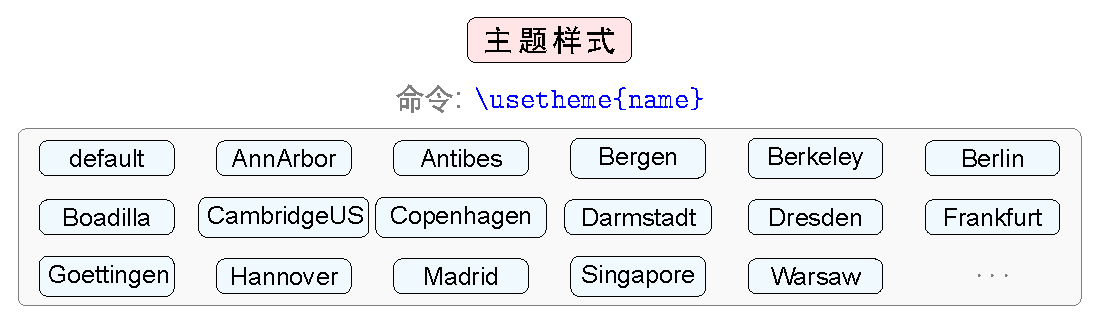
\includegraphics[width = 0.8\textwidth]{images/ch_9/beamer_theme.pdf}
    \caption{Beamer文档类型中的主题样式}
    \label{figeg:001}
\end{figure}

在Beamer文档类型中,有几十种主题样式可供选择和使用,比较常用的主题样式包括以下这些:
\begin{itemize}
    \item Berlin:柏林主题样式,默认样式为蓝色调;
    \item Copenhagen: 哥本哈根主题样式,默认样式为蓝色调;
    \item CambridgeUS:美国剑桥主题样式,默认样式为红色调;
    \item Berkeley:伯克利主题样式,默认样式为蓝色调;
    \item Singapore:新加坡主题样式;
    \item Warsaw:默认样式为蓝色调。
\end{itemize}

\emph{【例】}在beamer文档类型中使用CambridgeUS主题样式制作一个简单的幻灯片:
\begin{lstlisting}[language=TeX]
    \documentclass{beamer}
    \usetheme{CambridgeUS}
    
    \begin{document}
    
    \begin{frame}{Example}
    
    This is a simple example for the CambridgeUS theme.
    
    \end{frame}
    
    \end{document}
\end{lstlisting}

编译上述代码,得到幻灯片如图\ref{figeg:002}所示。

\begin{figure}[htbp]
    \centering
    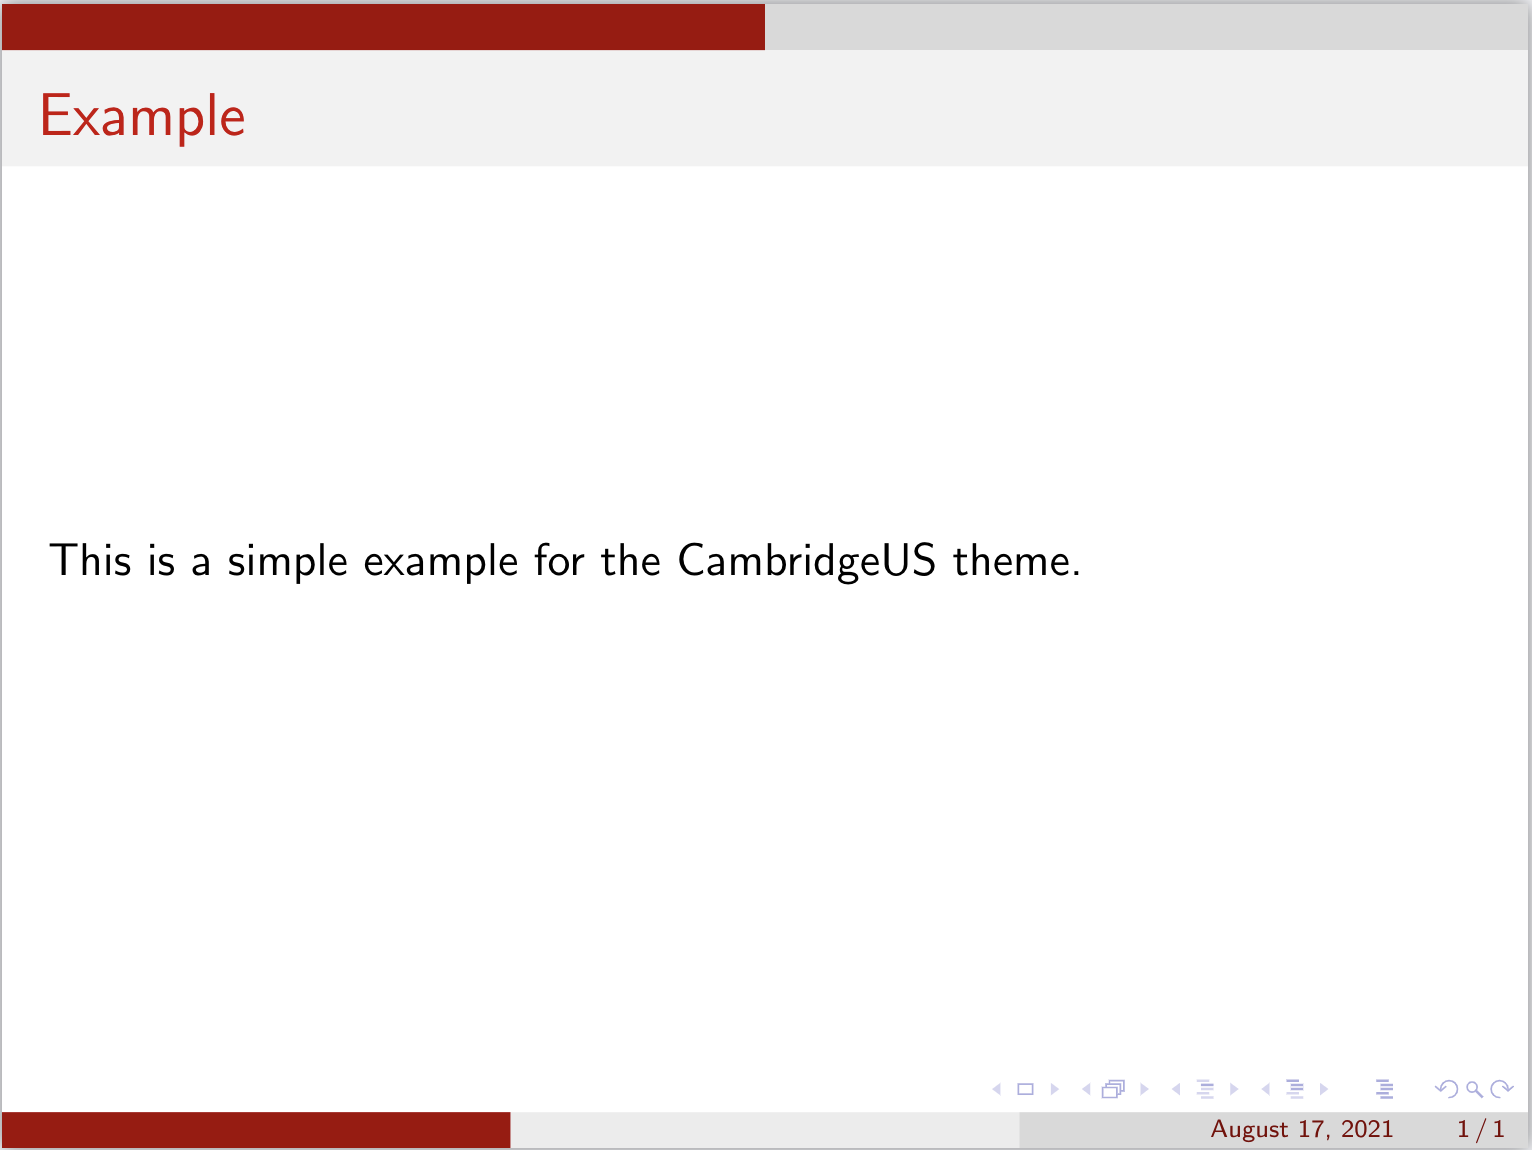
\includegraphics[width = 0.8\textwidth]{images/ch_9/example_sec2_1.png}
    \caption{编译后的幻灯片效果}
    \label{figeg:002}
\end{figure}

当然,在这些主题样式基础上,我们也能够使用一些特定的主题样式如颜色主题、字体主题、内部主题、外部主题对幻灯片的显示效果进行调整。

\begin{figure}[htbp]
    \centering
    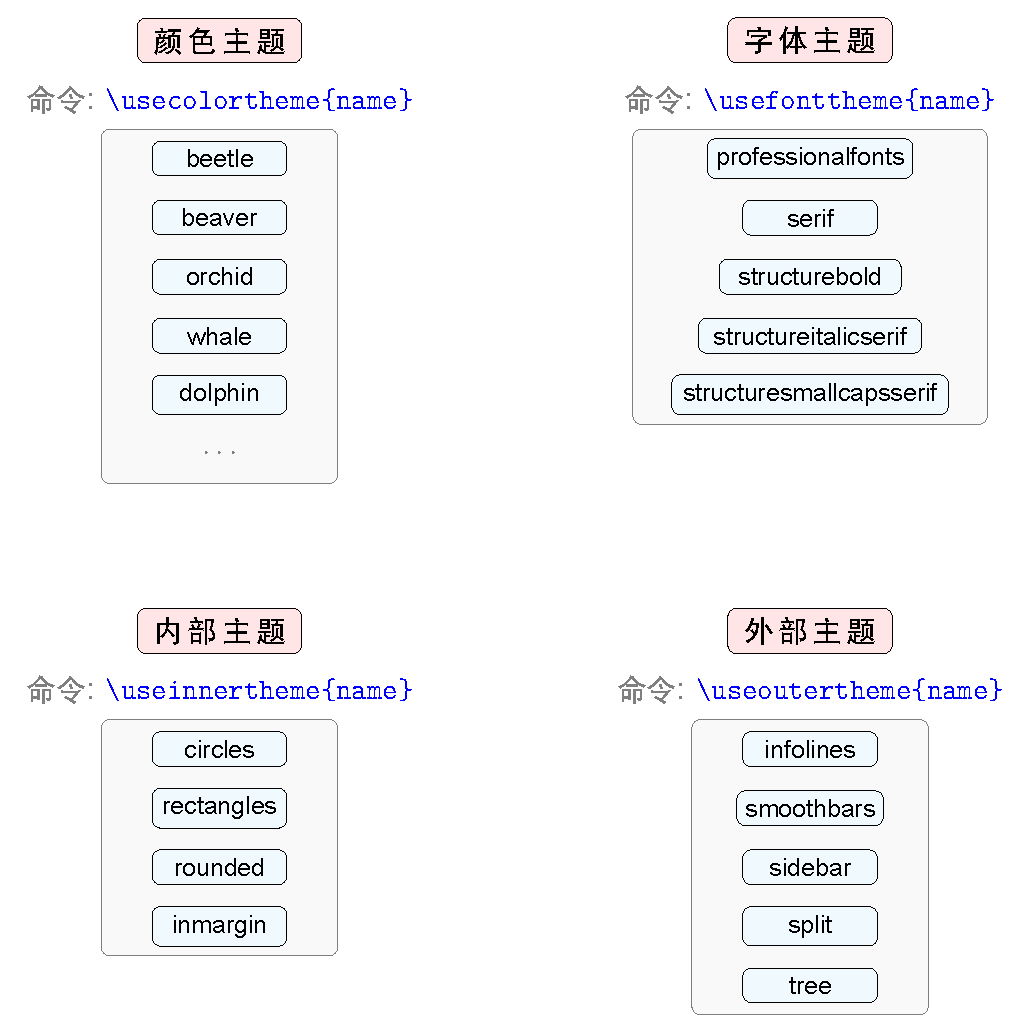
\includegraphics[width = 0.8\textwidth]{images/ch_9/other_themes.pdf}
    \caption{Beamer文档类型中的其他几种主题设置}
    \label{figeg:003}
\end{figure}

\subsection{颜色主题}

使用Beamer制作幻灯片时,我们能够自行设置幻灯片主题样式的色调,使用\texttt{\textbackslash{}usecolortheme\{\}}命令即可,这些色调包括beetle、beaver、orchid、whale、dolphin等。这里的色调又被称为颜色主题,它定义了幻灯片各部分的颜色搭配,设置特定的颜色主题后,我们能够得到不同的组合样式,具体可参考https://hartwork.org/beamer-theme-matrix/网站提供的组合样式矩阵。

\emph{【例】}在beamer文档类型中使用CambridgeUS主题样式和dolphin色调制作一个简单的幻灯片:
\begin{lstlisting}[language=TeX]
    \documentclass{beamer}
    \usetheme{CambridgeUS}
    \usecolortheme{dolphin}

    \begin{document}

    \begin{frame}{Example}

    This is a simple example for the CambridgeUS theme with dolphin (color theme).

    \end{frame}

    \end{document}
\end{lstlisting}

编译上述代码,得到幻灯片如图\ref{figeg:003}所示。

\begin{figure}[htbp]
    \centering
    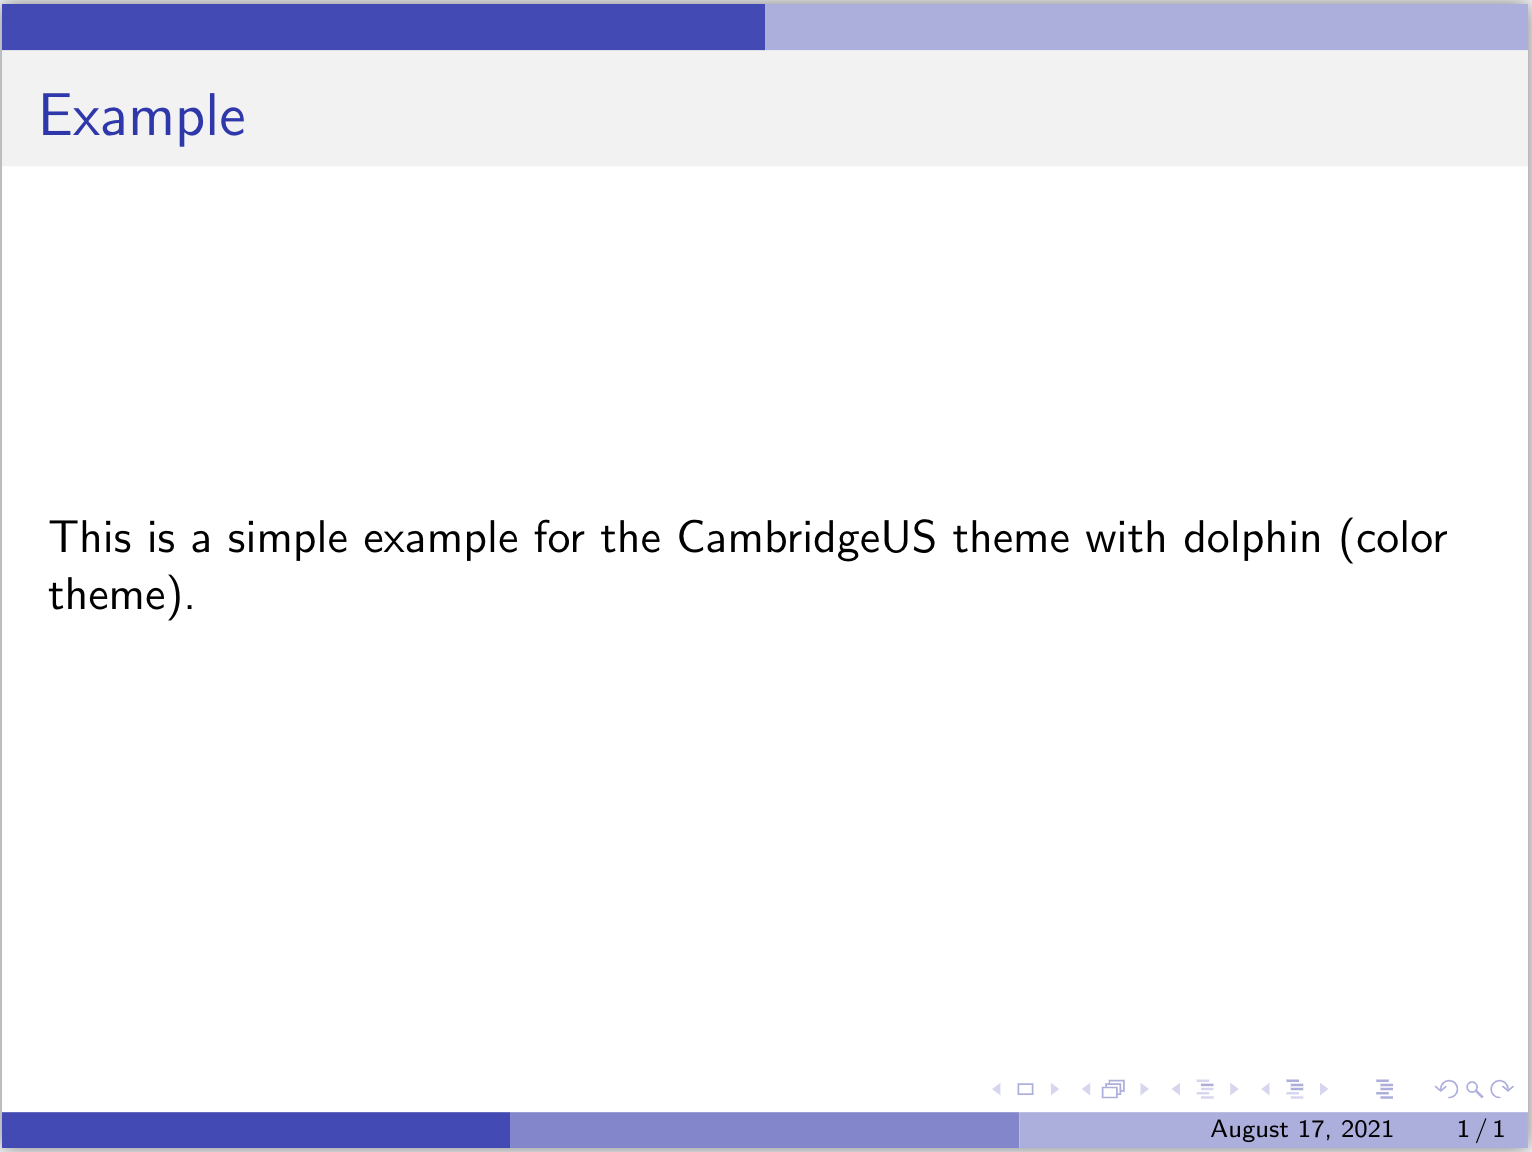
\includegraphics[width = 0.8\textwidth]{images/ch_9/example_sec2_2.png}
    \caption{编译后的幻灯片效果}
    \label{figeg:003}
\end{figure}

\subsection{字体主题}

实际上,对于幻灯片的文本字体,我们可以调用字体样式对其进行调整。在Beamer中,字体样式被称为字体主题,它定义了幻灯片的字体搭配。具体使用方法是:在前导代码中要用到的命令为\texttt{\textbackslash{}usefonttheme{A}},位置A填写的一般是字体类型,例如serif。

\emph{【例】}使用beamer文档类型创建一个简单的幻灯片,并在前导代码中申明使用serif对应的字体样式:
\begin{lstlisting}[language=TeX]
    \documentclass{beamer}
    \usefonttheme{serif}

    \begin{document}

    \begin{frame}

    This is a simple example for using \alert{serif} font theme.

    \end{frame}

    \end{document}
\end{lstlisting}

编译上述代码,得到幻灯片如图\ref{figeg:004}所示。

\begin{figure}[htbp]
    \centering
    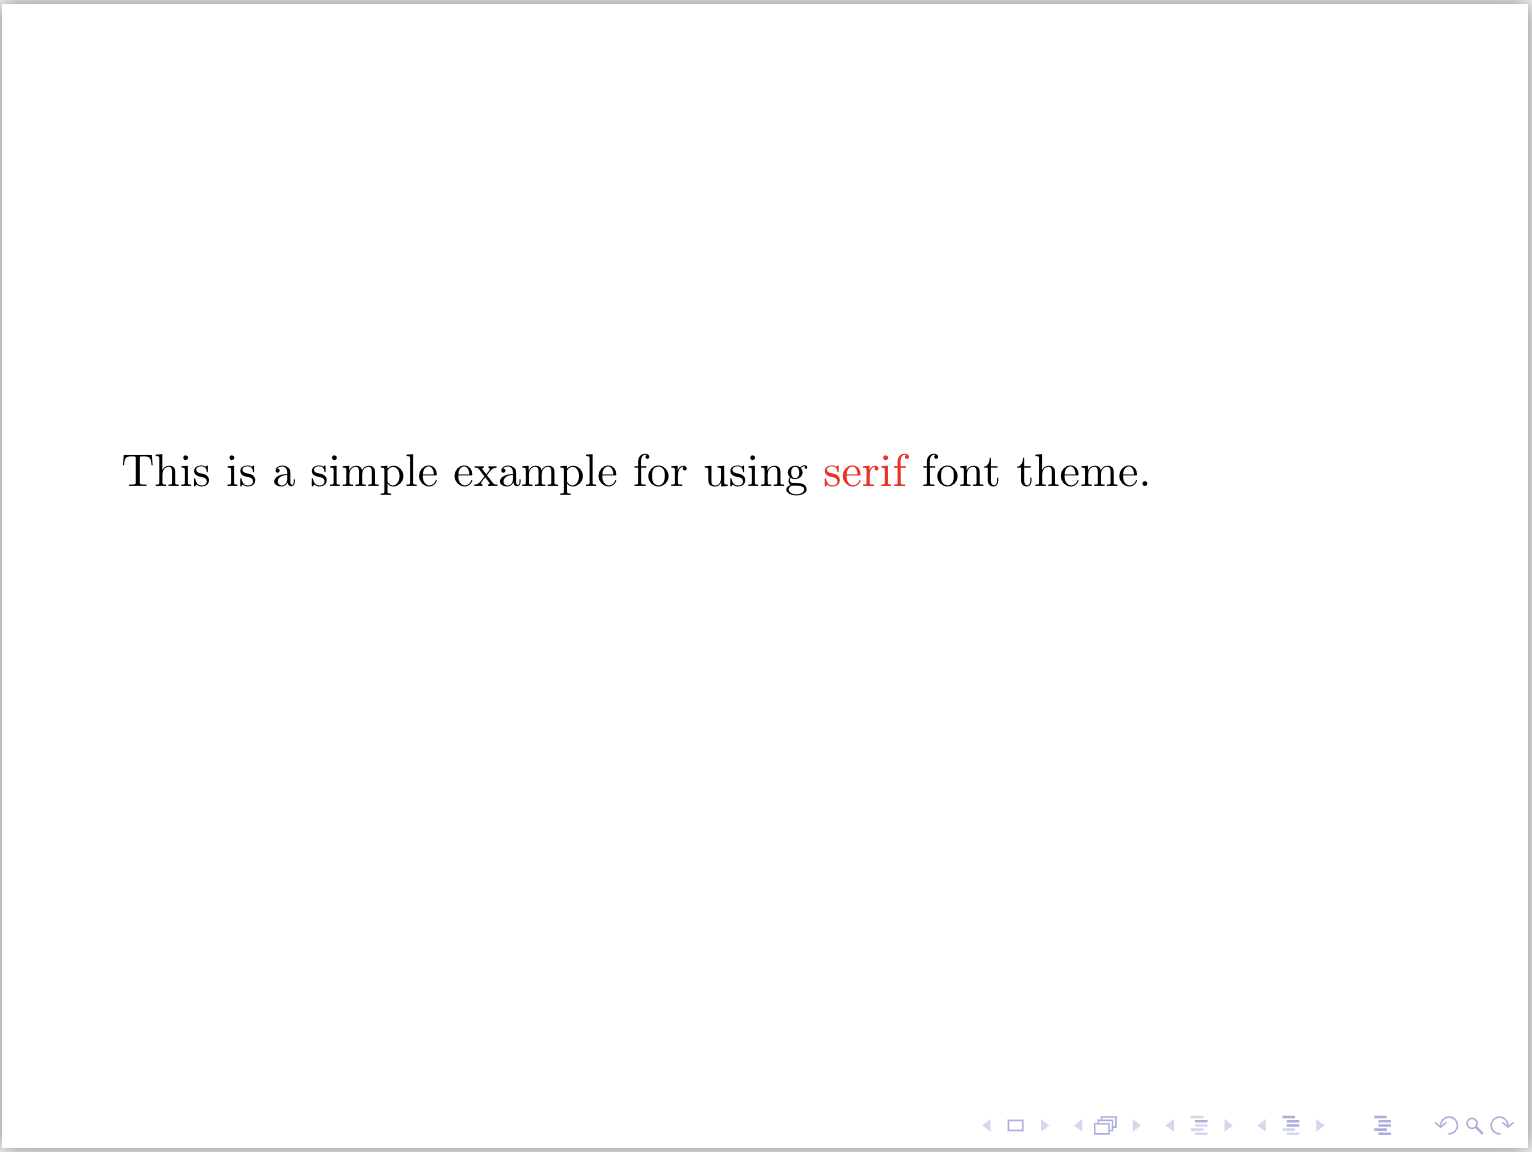
\includegraphics[width = 0.8\textwidth]{images/ch_9/example_sec2_3.png}
    \caption{编译后的幻灯片效果}
    \label{figeg:004}
\end{figure}

我们知道:在常规文档中,可以使用各种字体对应的宏包达到调用字体的作用,使用规则为\texttt{\textbackslash{}usepackage\{A\}},位置A填写的一般是字体类型,包括serif、avant、bookman、chancery、charter、euler、helvet、mathtime、mathptm、mathptmx、newcent、palatino、pifont、utopia等。

\emph{【例】}使用beamer文档类型创建一个简单的幻灯片,并在前导代码中申明使用字体palatino对应的宏包:
\begin{lstlisting}[language=TeX]
    \documentclass{beamer}
    \usepackage{palatino}

    \begin{document}

    \begin{frame}

    This is a simple example for using \alert{palatino} font.

    \end{frame}

    \end{document}
\end{lstlisting}

编译上述代码,得到幻灯片如图\ref{figeg:005}所示。

\begin{figure}[htbp]
    \centering
    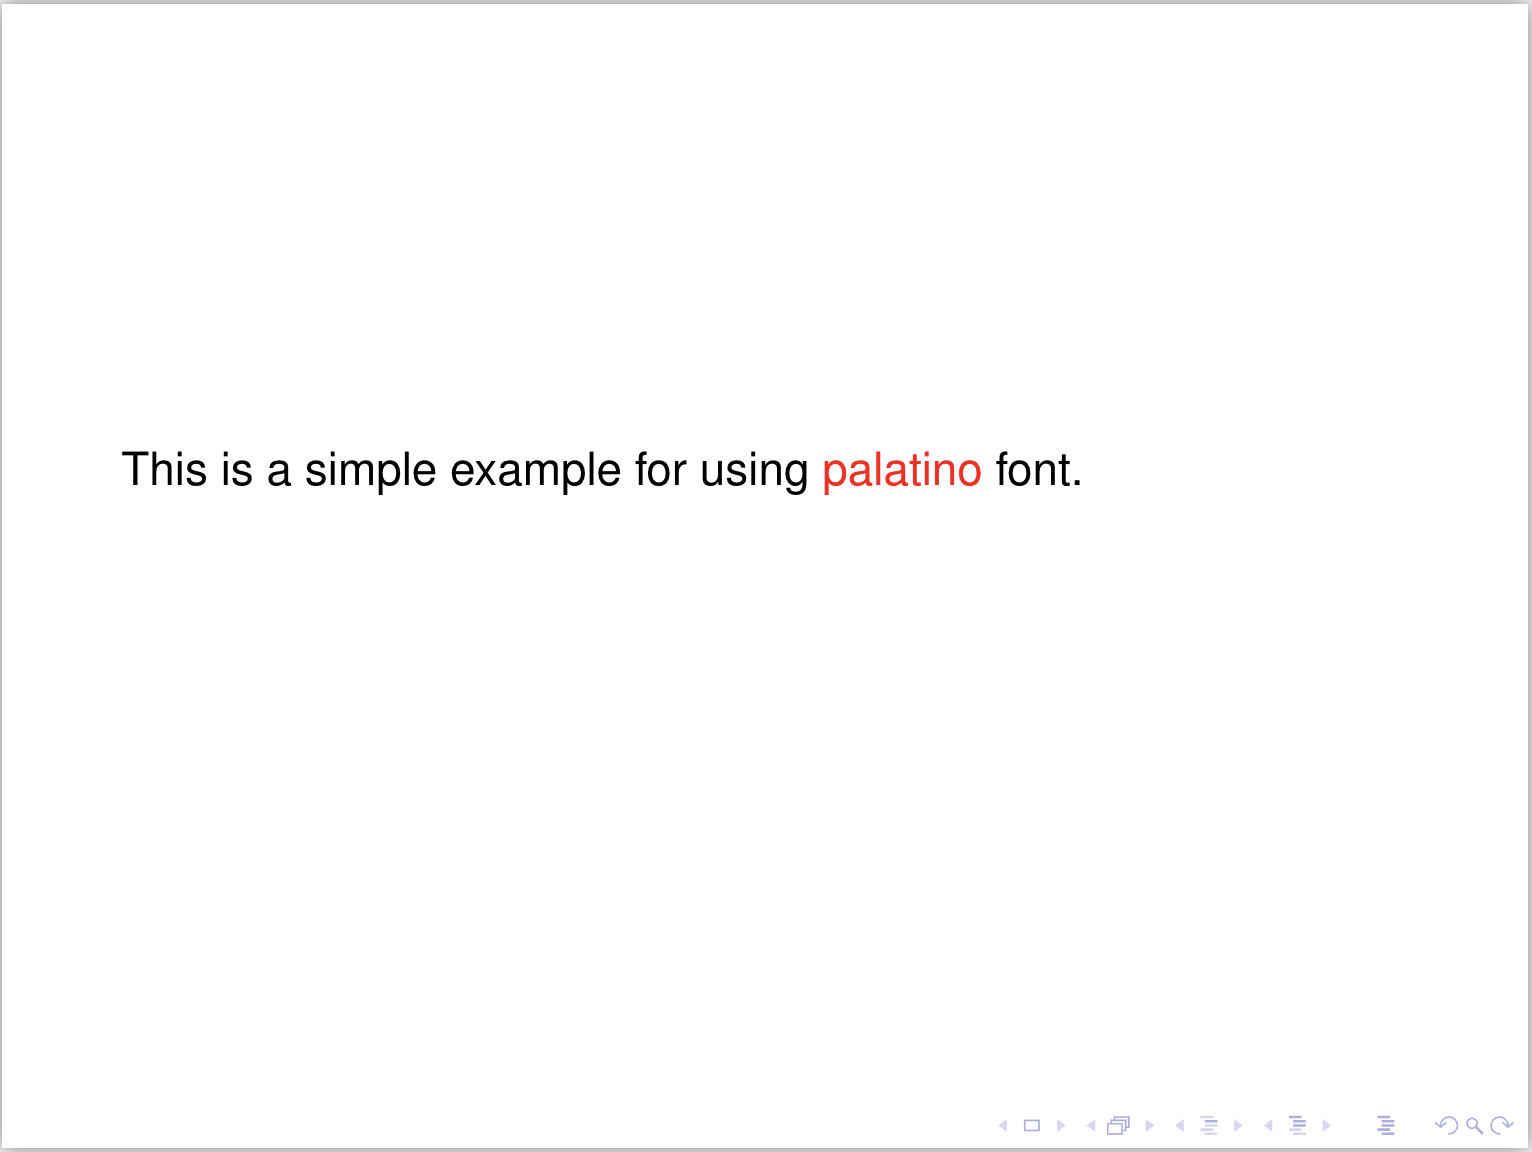
\includegraphics[width = 0.8\textwidth]{images/ch_9/example_sec2_4.png}
    \caption{编译后的幻灯片效果}
    \label{figeg:005}
\end{figure}

\subsection{内部主题}

内部主题定义了幻灯片展示区域的样式,如列表、定理等,内部主题不包括页眉、页脚、导航栏等部分。每一种主题样式都有默认的内部主题,更换内部主题需使用\texttt{\textbackslash{}useinnertheme\{A\}}命令,位置A可供选择的内部主题包括circles、rectangles、rounded和inmargin。

\emph{【例】}在beamer文档类型中分别使用circles内部主题制作幻灯片:
\begin{lstlisting}[language=TeX]
    \documentclass{beamer}
    \usetheme{CambridgeUS}
    \usefonttheme{professionalfonts}
    \useinnertheme{circles}

    \begin{document}

    \begin{frame}
    \frametitle{Parent function}
    \framesubtitle{A short list}

    Please check out the following parent function list.
    \begin{enumerate}
    \item $y=x$
    \item $y=|x|$
    \item $y=x^{2}$
    \item $y=x^{3}$
    \item $y=x^{b}$
    \end{enumerate}

    \end{frame}

    \end{document}
\end{lstlisting}

编译上述代码,得到幻灯片如图\ref{figeg:006}所示。

\begin{figure}[htbp]
    \centering
    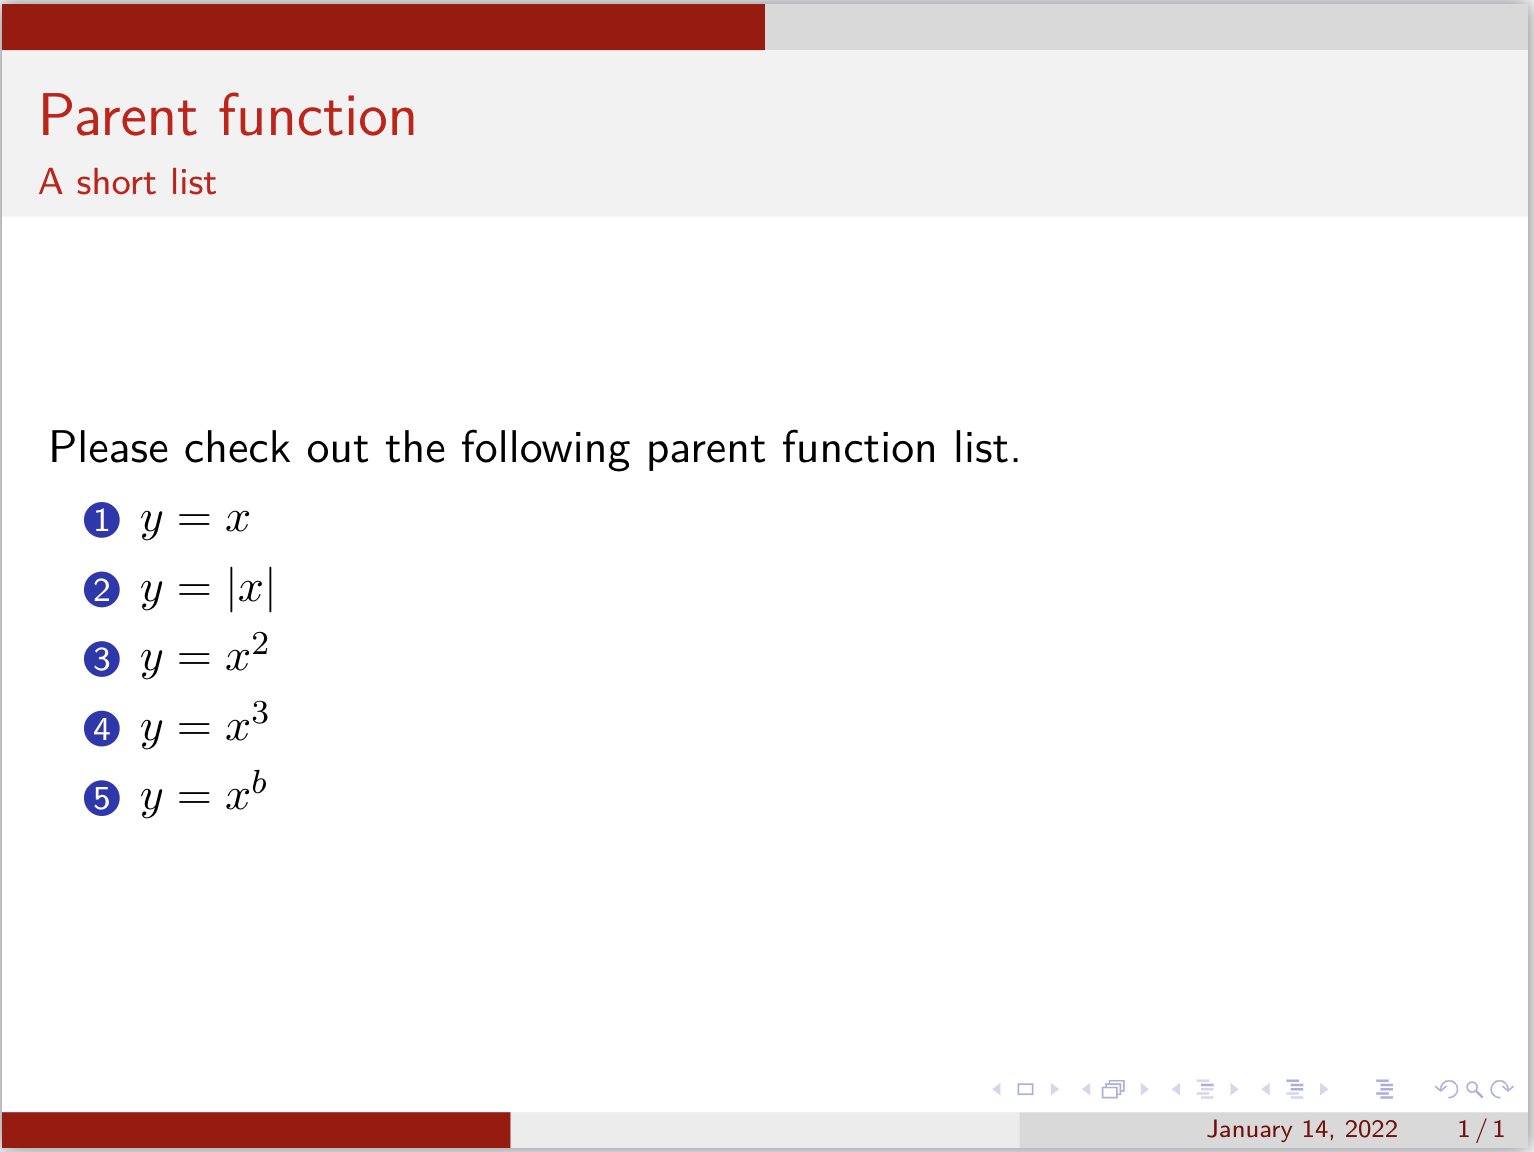
\includegraphics[width = 0.8\textwidth]{images/ch_9/example_innertheme_circles.png}
    \caption{编译后的幻灯片效果}
    \label{figeg:006}
\end{figure}

\emph{【例】}在beamer文档类型中分别使用inmargin内部主题制作幻灯片:
\begin{lstlisting}[language=TeX]
    \documentclass{beamer}
    \usetheme{CambridgeUS}
    \usefonttheme{professionalfonts}
    \useinnertheme{inmargin}

    \begin{document}

    \begin{frame}
    \frametitle{Parent function}
    \framesubtitle{A short list}

    Please check out the following parent function list.
    \begin{enumerate}
    \item $y=x$
    \item $y=|x|$
    \item $y=x^{2}$
    \item $y=x^{3}$
    \item $y=x^{b}$
    \end{enumerate}

    \end{frame}

    \end{document}
\end{lstlisting}

编译上述代码,得到幻灯片如图\ref{figeg:007}所示。

\begin{figure}[htbp]
    \centering
    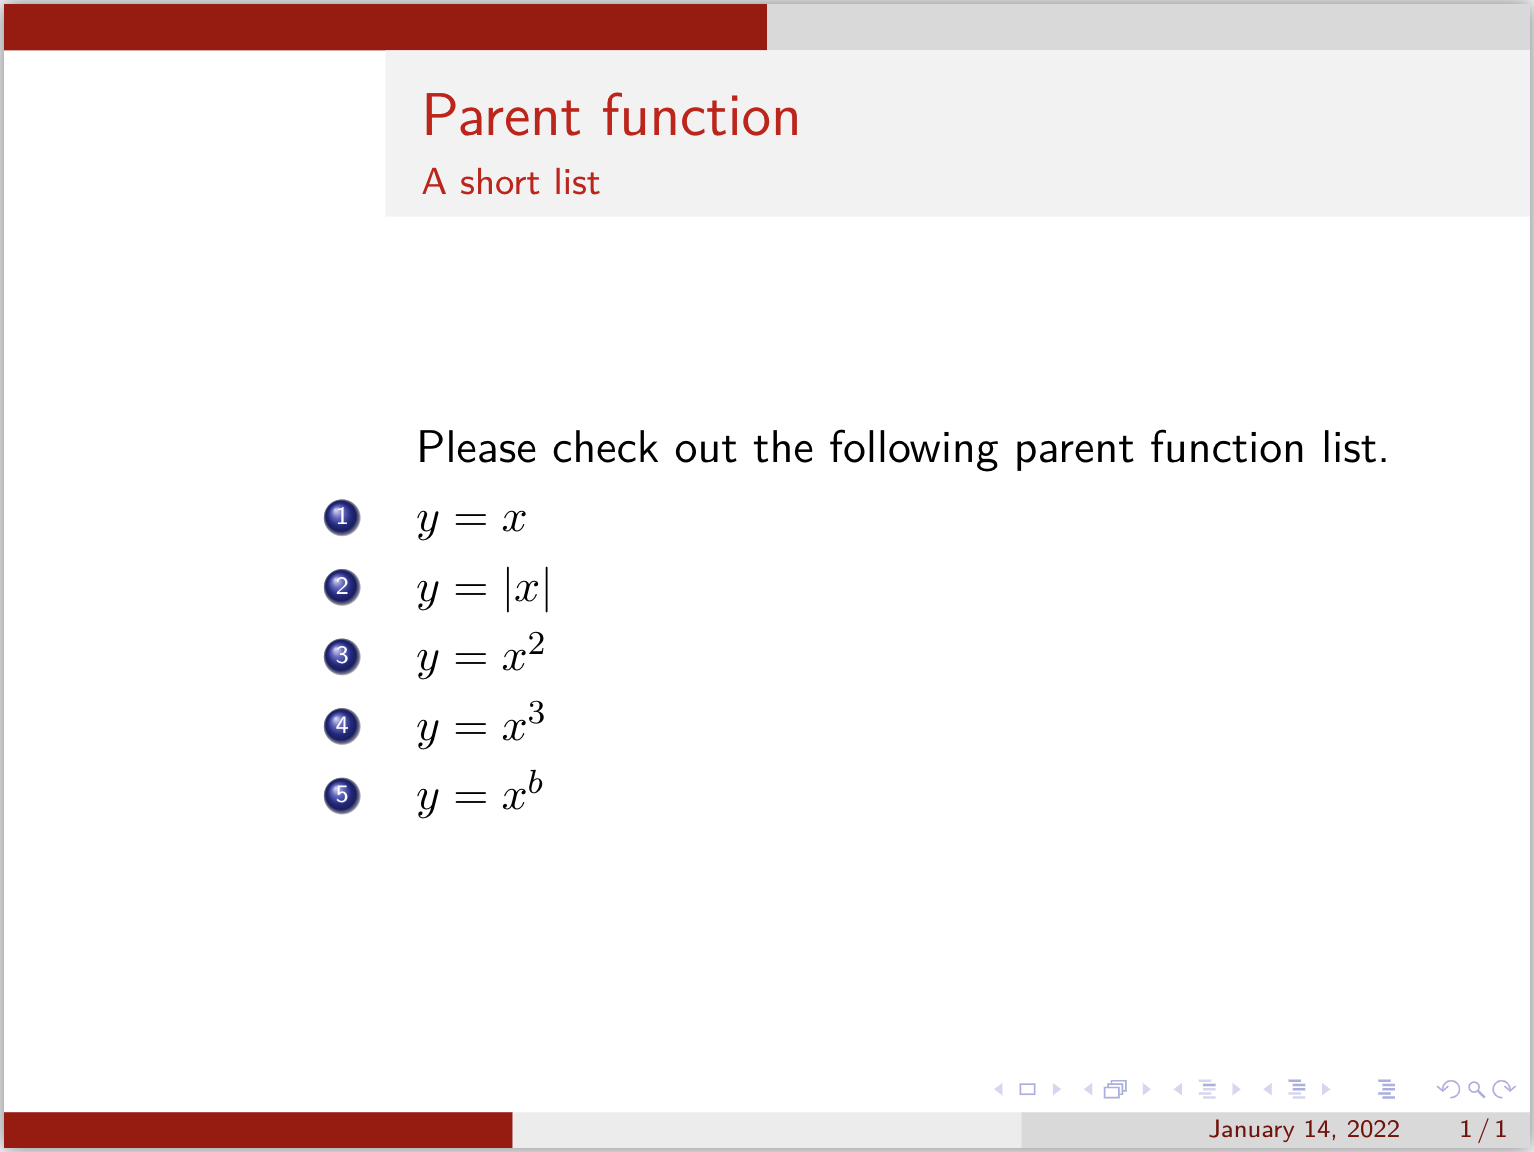
\includegraphics[width = 0.8\textwidth]{images/ch_9/example_innertheme_inmargin.png}
    \caption{编译后的幻灯片效果}
    \label{figeg:007}
\end{figure}

\subsection{外部主题}

外部主题定义了幻灯片的边框、页眉、页脚、导航栏等部分的样式。更换外部主题需使用\texttt{\textbackslash{}useoutertheme\{A\}},位置A可供选择的外部主题包括infolines、smoothbars、sidebar、split和tree。

\subsection{表格字体大小}

在Beamer中制作表格,当我们想对表头或者表格内容文字大小进行调整时,可以使用在前导代码中申明使用\emph{caption}宏包,即\texttt{\textbackslash{}usepackage\{caption\}},然后设置具体的字体大小即可,如\texttt{\textbackslash{}captionsetup\{font = scriptsize, labelfont = scriptsiz\}}可以将表头和表格内容字体大小调整为scriptsize。

\emph{【例】}使用table环境创建一个简单表格,并使用caption宏包将表头字体大小设置为Large、将表格内容字体大小设置为large:
\begin{lstlisting}[language=TeX]
    \documentclass{beamer}
    \usepackage{booktabs}
    \usepackage{caption}
    \captionsetup{font = large, labelfont = Large}

    \begin{document}

    \begin{frame}

    \begin{table}
    \caption{A simple table.}
    \begin{tabular}{l|ccc}
    \toprule
    & \textbf{header3} & \textbf{header4} & \textbf{header5} \\
    \midrule
    \textbf{header1} & cell1 & cell2 & cell3 \\
    \midrule
    \textbf{header2} & cell4 & cell5 & cell6 \\
    \bottomrule
    \end{tabular}
    \end{table}

    \end{frame}

    \end{document}
\end{lstlisting}

编译上述代码,得到幻灯片如图\ref{figeg:008}所示。

\begin{figure}[htbp]
    \centering
    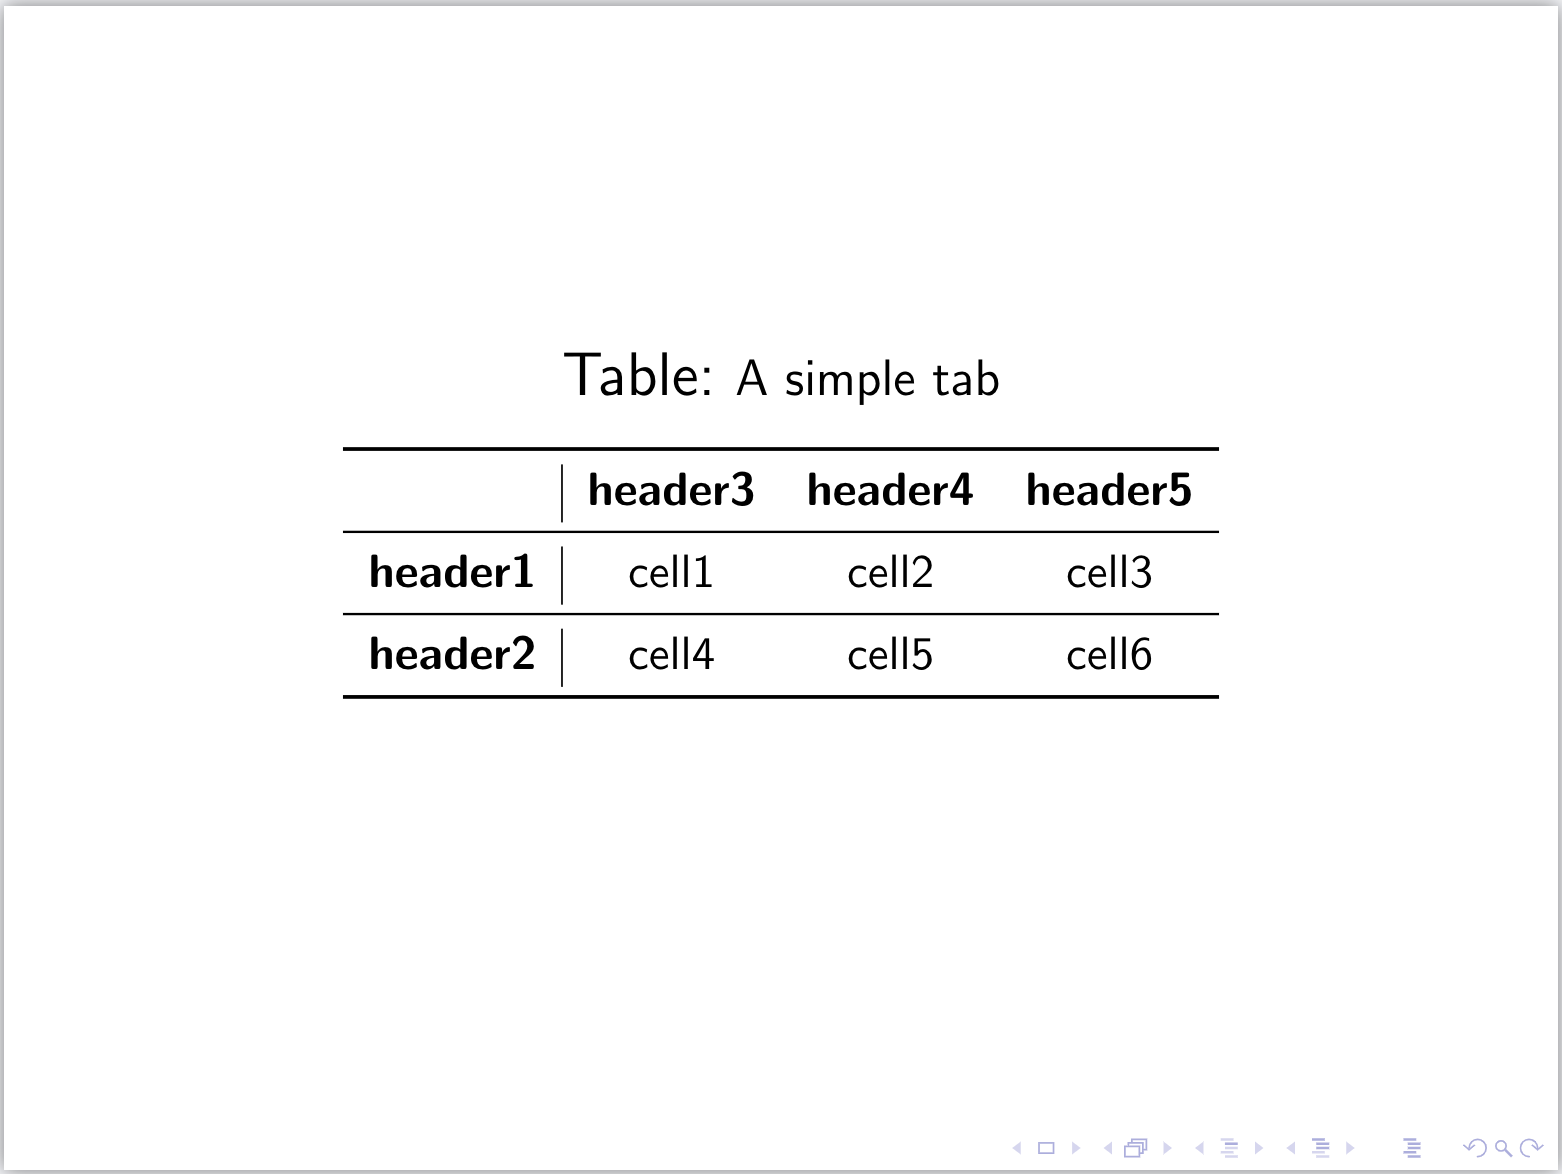
\includegraphics[width = 0.8\textwidth]{images/ch_9/example_sec2_5.png}
    \caption{编译后的幻灯片效果}
    \label{figeg:008}
\end{figure}

其中,单就设置表头字体大小而言,除了使用caption宏包之外,还可以通过对幻灯片设置全局参数达到调整字体大小的效果,例如\texttt{\textbackslash{}setbeamerfont\{caption\}\{size = \textbackslash{}Large\}}。

\subsection{样式调整}

在Beamer文档类型中,除了可以使用各种主题样式,另外也可以根据幻灯片组成部分,分别对侧边栏、导航栏以及Logo等进行调整。其中,侧边栏是由所选幻灯片主题样式自动生成的,主要用于显示幻灯片目录。有时为了显示幻灯片的层次,使用侧边栏进行目录索引。

\emph{【例】}使用Berkeley主题样式,并将侧边栏显示在右侧:
\begin{lstlisting}[language=TeX]
    \documentclass{beamer}
    \PassOptionsToPackage{right}{beamerouterthemesidebar}
    \usetheme{Berkeley}
    \usefonttheme{professionalfonts}

    \begin{document}

    \begin{frame}
    \frametitle{Parent function}
    \framesubtitle{A short list}

    Please check out the following parent function list.
    \begin{enumerate}
    \item $y=x$
    \item $y=|x|$
    \item $y=x^{2}$
    \item $y=x^{3}$
    \item $y=x^{b}$
    \end{enumerate}

    \end{frame}

    \end{document}
\end{lstlisting}

编译上述代码,得到幻灯片如图\ref{figeg:009}所示。

\begin{figure}[htbp]
    \centering
    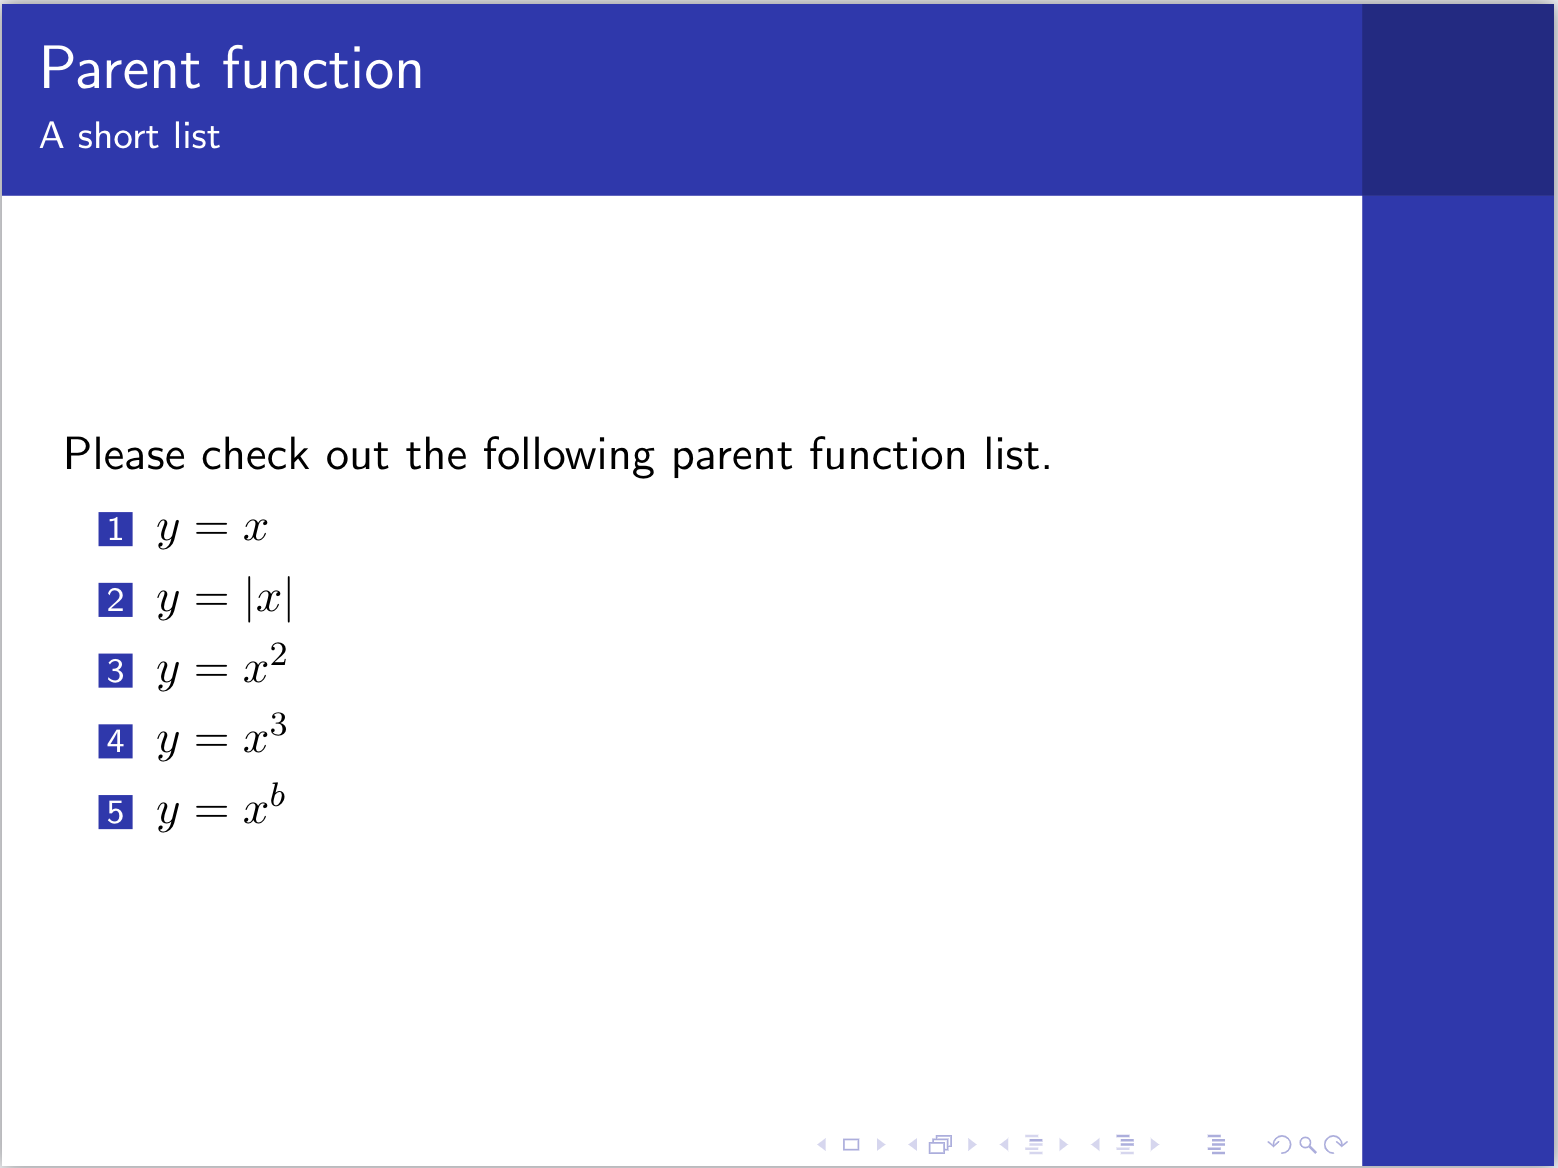
\includegraphics[width = 0.8\textwidth]{images/ch_9/example_sec2_6.png}
    \caption{编译后的幻灯片效果}
    \label{figeg:009}
\end{figure}

很多时候我们会发现,在各类学术汇报中,幻灯片的首页通常会有主讲人所在的研究机构Logo。在Beamer文档类型中,有\texttt{\textbackslash{}logo}和\texttt{\textbackslash{}titlegraphic}两个命令可供使用,使用\texttt{\textbackslash{}logo}命令添加的Logo会在每一页幻灯片中都显示,而使用\texttt{\textbackslash{}titlegraphic}命令添加的Logo只出现在标题页。

\emph{【例】}使用logo命令在幻灯片中添加Logo:
\begin{lstlisting}[language=TeX]
    \documentclass{beamer}
    \usefonttheme{professionalfonts}

    \title{A Simple Beamer Example}
    \author{Author's Name}
    \institute{Author's Institute}

    \logo{\includegraphics[width=2cm]{logopolito}}

    \begin{document}

    \begin{frame}
    \titlepage
    \end{frame}

    \begin{frame}{Parent function}{A short list}
    Please check out the following parent function list.
    \begin{enumerate}
    \item $y=x$
    \item $y=|x|$
    \item $y=x^{2}$
    \item $y=x^{3}$
    \item $y=x^{b}$
    \end{enumerate}
    \end{frame}

    \end{document}
\end{lstlisting}

编译上述代码,得到幻灯片如图\ref{figeg:010}所示。

\begin{figure}[htbp]
    \centering
    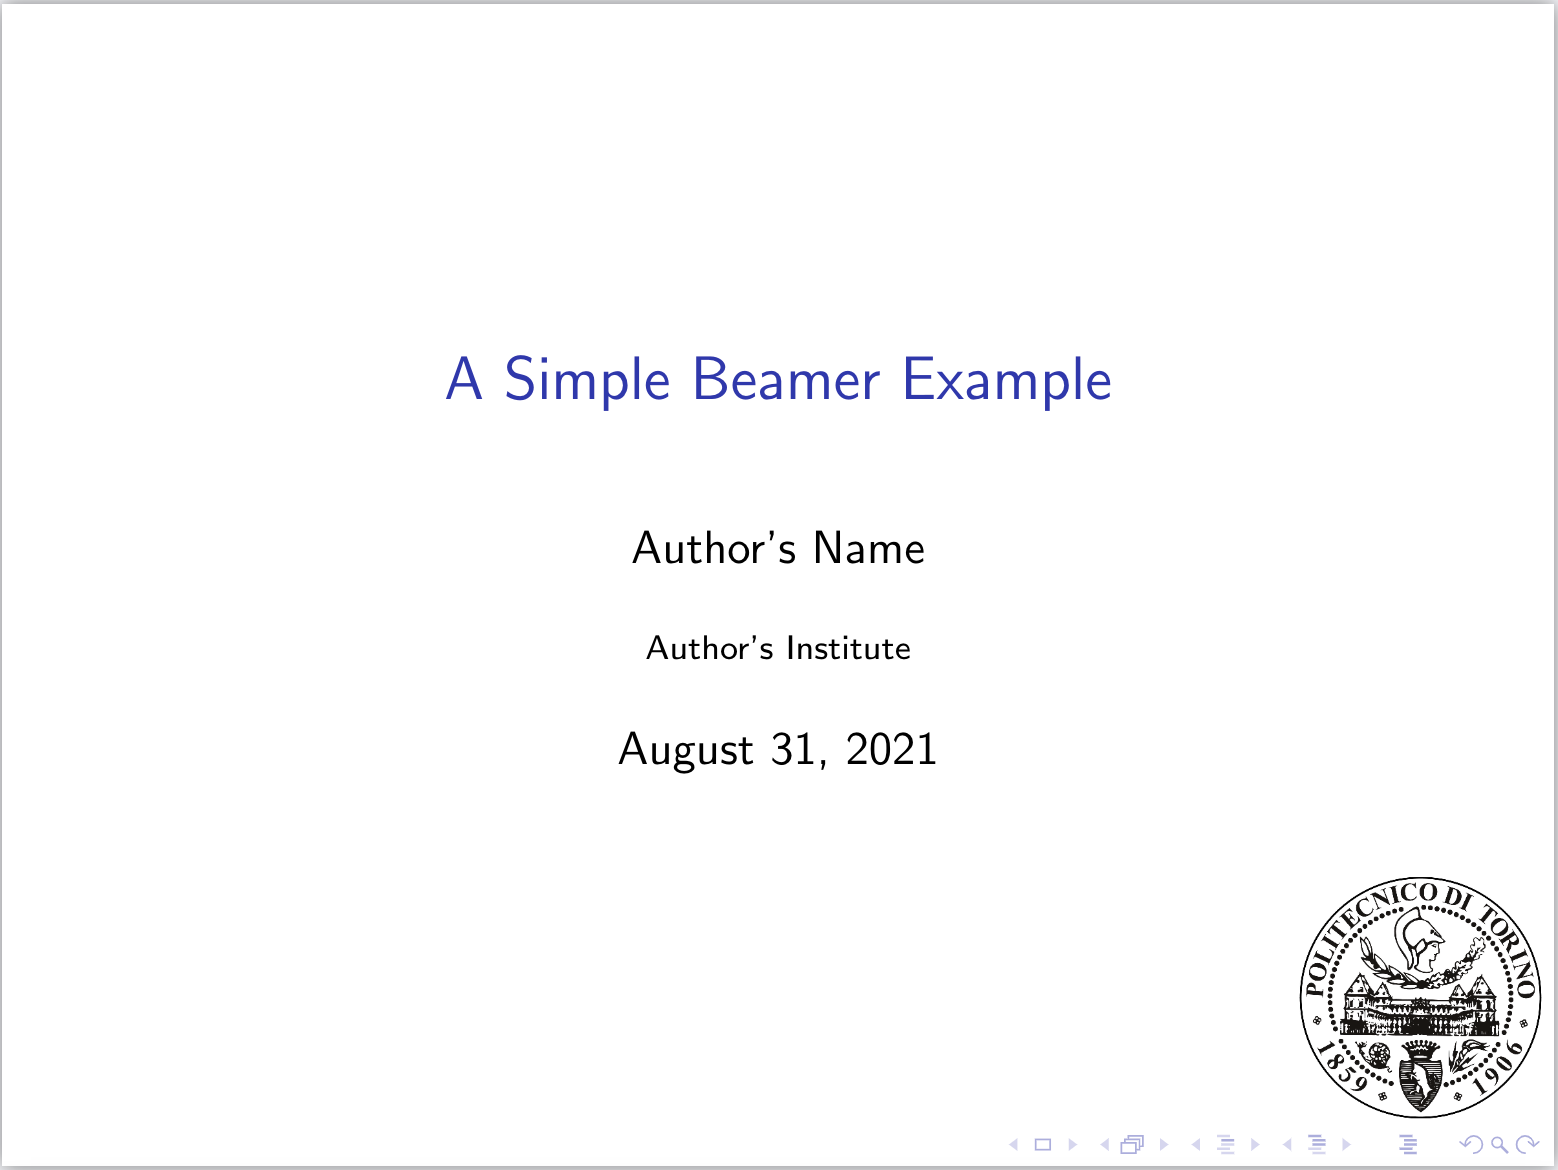
\includegraphics[width = 0.45\textwidth]{images/ch_9/example_sec2_7_0.png}
    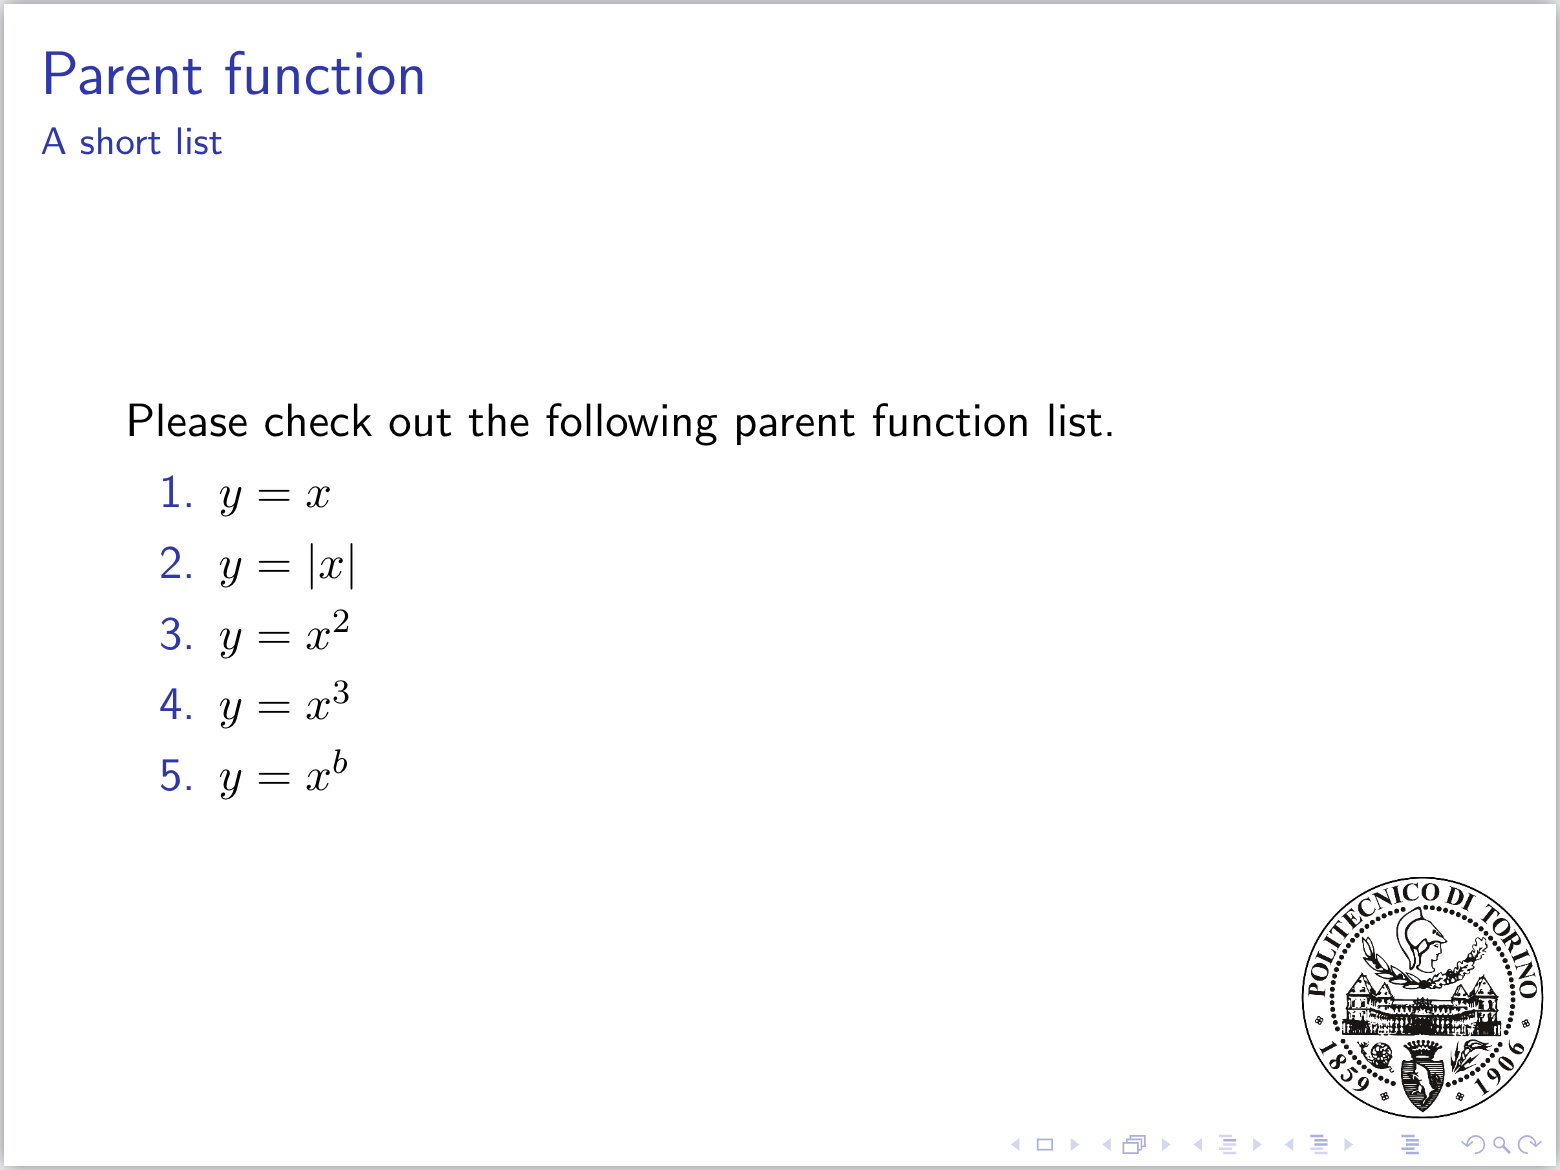
\includegraphics[width = 0.45\textwidth]{images/ch_9/example_sec2_7_1.png}
    \caption{编译后的幻灯片效果}
    \label{figeg:010}
\end{figure}

\emph{【例】}使用titlegraphic命令在幻灯片的标题页添加Logo:
\begin{lstlisting}[language=TeX]
    \documentclass{beamer}
    \usefonttheme{professionalfonts}

    \title{A Simple Beamer Example}
    \author{Author's Name}
    \institute{Author's Institute}

    \titlegraphic{\includegraphics[width=2cm]{logopolito}\hspace*{4.75cm}~
    \includegraphics[width=2cm]{logopolito}
    }

    \begin{document}

    \begin{frame}
    \titlepage
    \end{frame}

    \begin{frame}{Parent function}{A short list}
    Please check out the following parent function list.
    \begin{enumerate}
    \item $y=x$
    \item $y=|x|$
    \item $y=x^{2}$
    \item $y=x^{3}$
    \item $y=x^{b}$
    \end{enumerate}
    \end{frame}

    \end{document}
\end{lstlisting}

编译上述代码,得到幻灯片如图\ref{figeg:011}所示。

\begin{figure}[htbp]
    \centering
    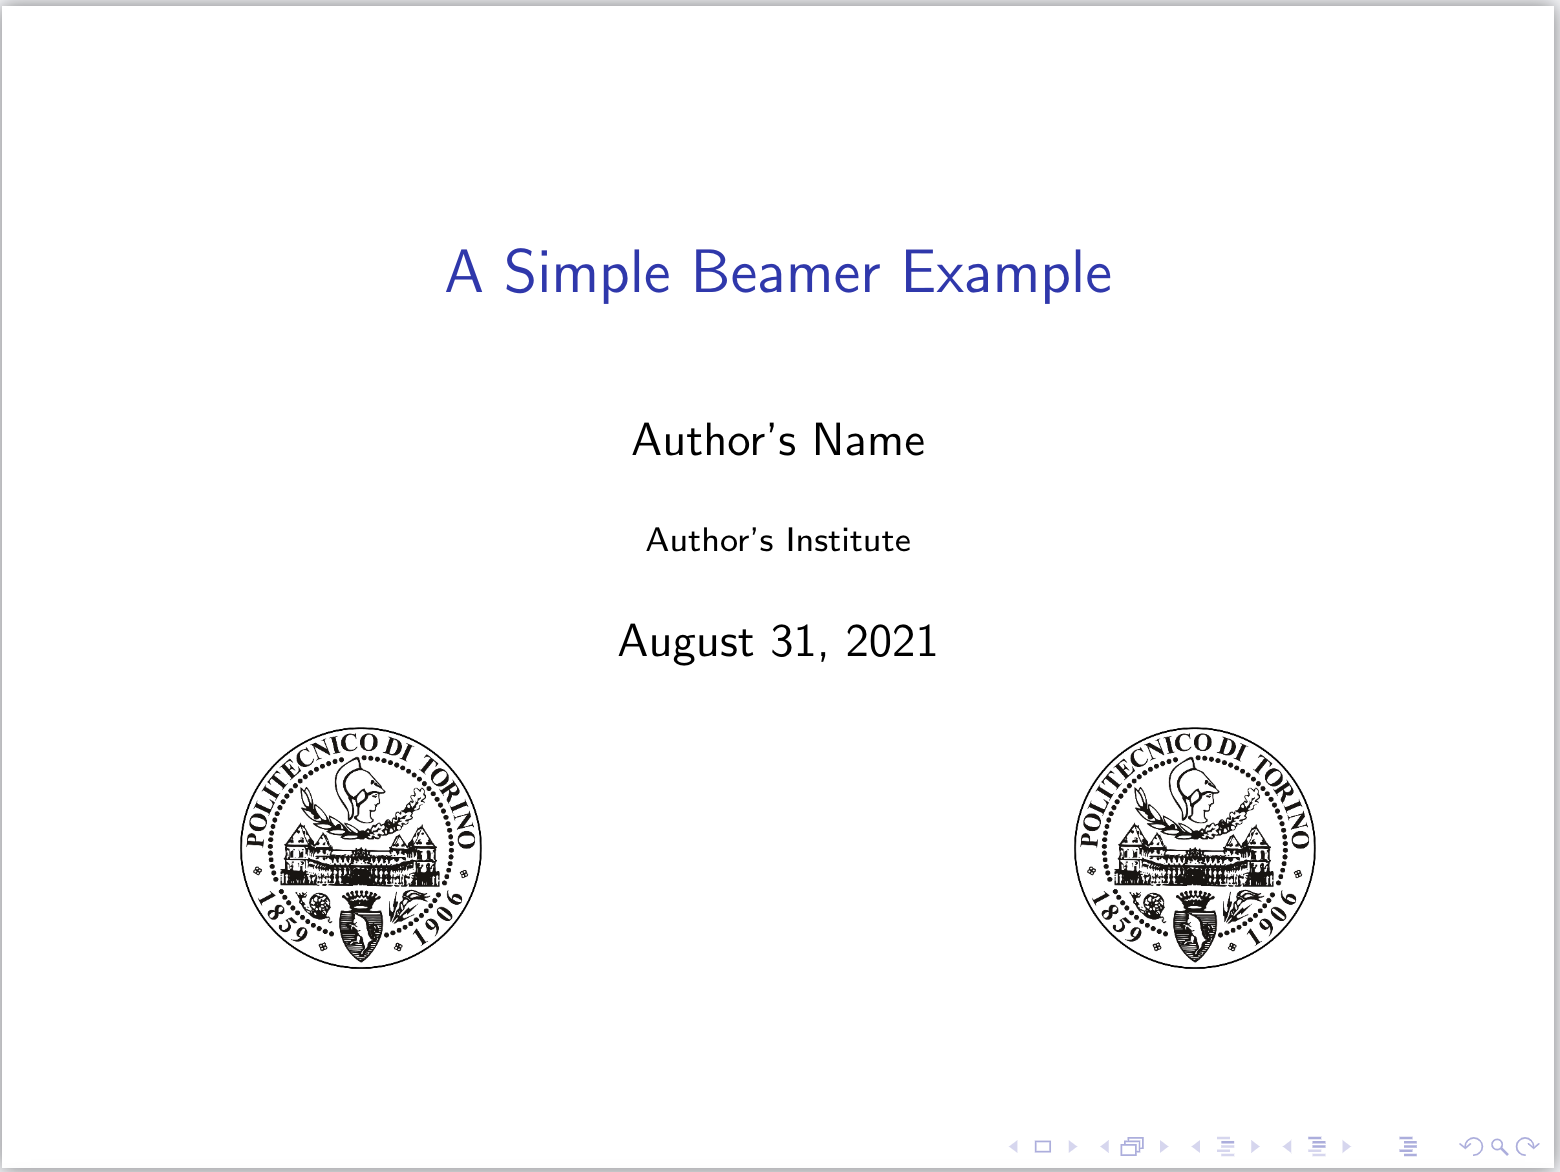
\includegraphics[width = 0.45\textwidth]{images/ch_9/example_sec2_8_0.png}
    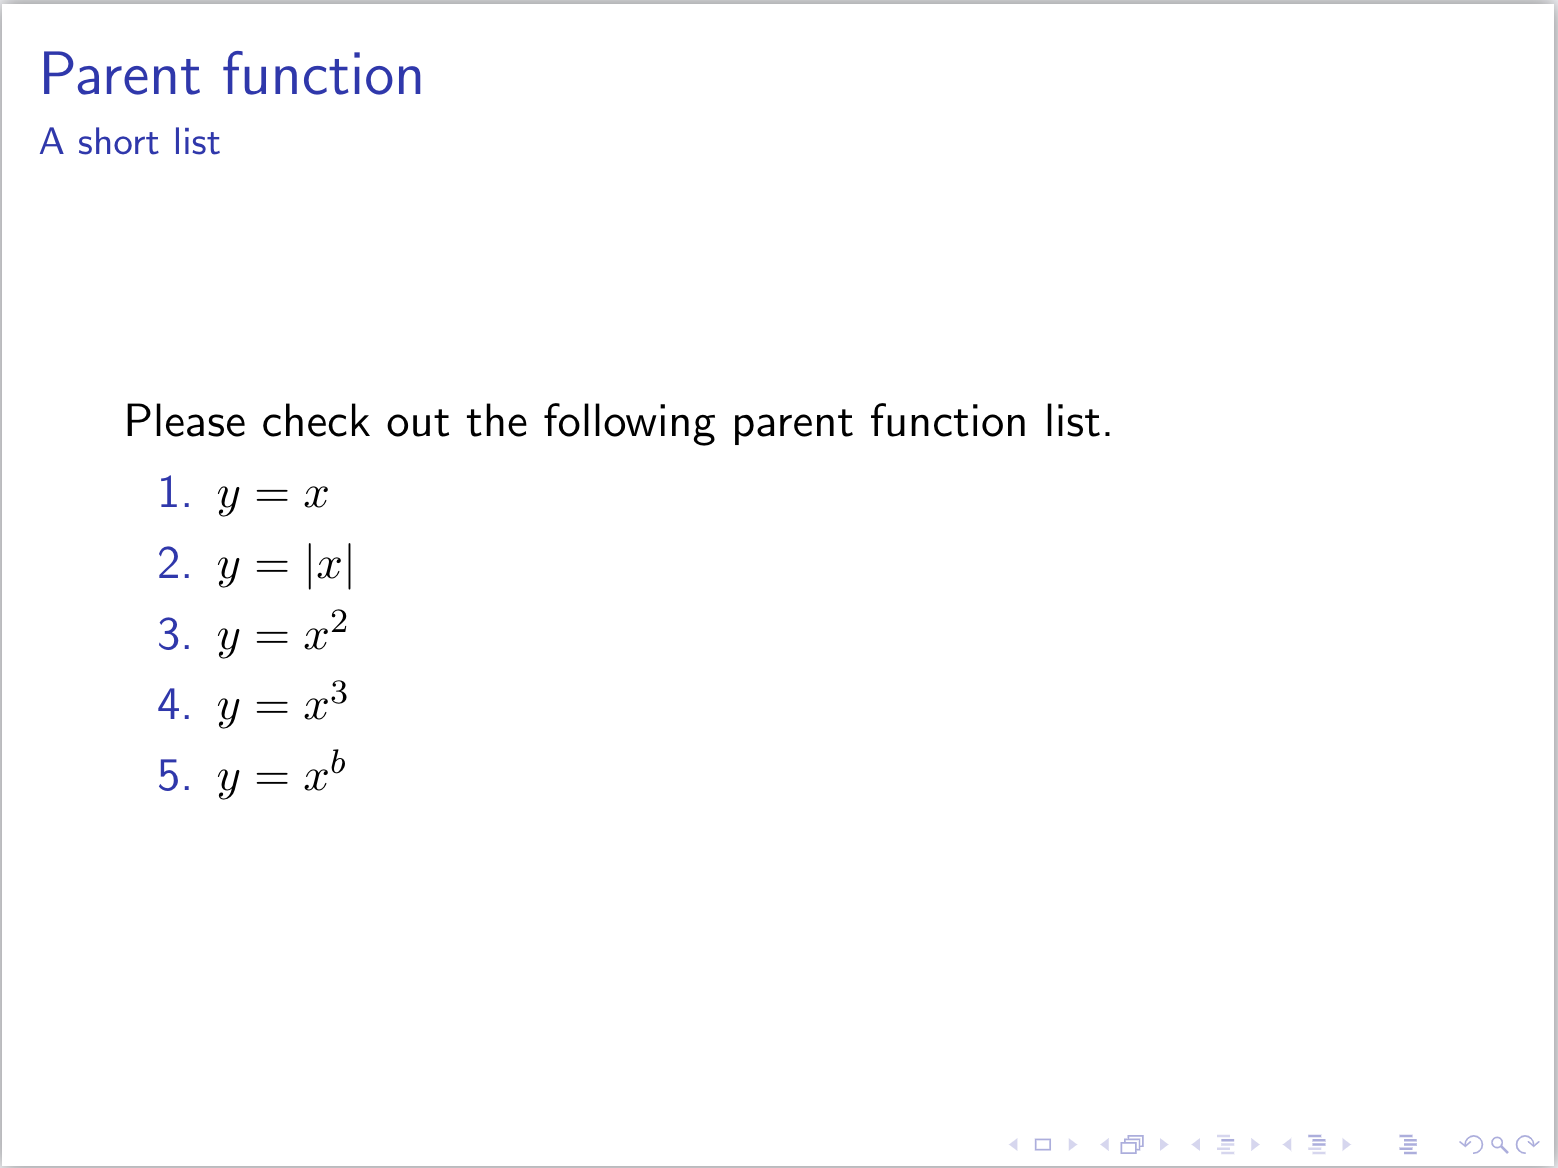
\includegraphics[width = 0.45\textwidth]{images/ch_9/example_sec2_8_1.png}
    \caption{编译后的幻灯片效果}
    \label{figeg:011}
\end{figure}
\end{document}